%%%%%%%%%%%%%%%%%%%%%%%%%%%%%%%%%%%%%%%%%%%%
% Main document
%%%%%%%%%%%%%%%%%%%%%%%%%%%%%%%%%%%%%%%%%%%%
\documentclass[a4paper,11pt,twoside,openright]{book}

%%%%%%%%%%%%%%%%%%%%%%%%%%%%%%%%%%%%%%%%
%           Liste des packages         %
%%%%%%%%%%%%%%%%%%%%%%%%%%%%%%%%%%%%%%%%


%% Réglage des fontes et typo
%\usepackage[utf8]{inputenc}
%\usepackage[T1]{fontenc}
%\usepackage[frenchb]{babel}
%
%\usepackage{mathptmx}
%\usepackage{avant}



%% Apparence globale
\usepackage{color}
\usepackage[top=1.5cm, bottom=3.5cm, inner=2cm, outer=3cm]{geometry}

% \usepackage[french]{minitoc}		% Permet de faire une table des matieres par chapitre
% \setcounter{minitocdepth}{3}		% Mini-toc détaillées (sections/sous-sections)
% \usepackage{silence}
% \WarningFilter{minitoc(hints)}{W0023}	% Virer les erreur dues à minitoc
% \WarningFilter{minitoc(hints)}{W0024}
% \WarningFilter{minitoc(hints)}{W0028}
% \WarningFilter{minitoc(hints)}{W0030}
% \WarningFilter{blindtext}{} % this takes care of the `blindtext` messages

\usepackage{titlesec}
\usepackage{enumerate}
\usepackage{enumitem}
\usepackage{pdflscape}			% Permet d'utiliser des pages au format paysage
\usepackage{url}
\usepackage{listings}			% Permet d'insérer du code source
\usepackage{changepage}

\usepackage{natbib}
\usepackage{paralist}
\usepackage{aas_macros}

\usepackage{hyperref}
\definecolor{citations}{rgb}{0,0,0.4}
\definecolor{liens}{rgb}{0.5,0,0}
\hypersetup{
	bookmarks=false,
	unicode=true,
	pdffitwindow=true,
	pdfnewwindow=false,
	colorlinks=true,
	linkcolor=blue,
	citecolor=green,
	urlcolor=cyan}
% \usepackage{breakurl}
% \usepackage{ifmtarg}

%% Maths
\usepackage{amsmath}	% Permet de taper des formules mathématiques
\usepackage{amssymb}	% Permet d'utiliser des symboles mathématiques
\usepackage{amsfonts}	% Permet d'utiliser des polices mathématiques
\usepackage{amsthm}
\usepackage{nicefrac}	% Permet de taper de belles fractions
\usepackage{relsize}

\usepackage[ruled,vlined]{algorithm2e}
%\SetKwInput{Data}{\textbf{Données}}
%\SetKwInput{Res}{\textbf{Résultats}}
%\SetKwFor{Pour}{pour}{faire}{fin boucle}
%\SetKwBlock{Deb}{début}{fin}
%\SetKwInput{Entree}{Entrées}
%\SetKwInput{Sortie}{Sorties}
%%     \SetKw{KwA}{à}
%%     \SetKw{Retour}{retourner}
%%     \SetKwIF{Si}{SinonSi}{Sinon}{si}{alors}{sinon si}{alors}{finsi}
%%     \SetKwSwitch{Suivant}{Cas}{Autre}{suivant}{faire}{cas où}{autres cas}{fin d’alternative}
%%     \SetKwFor{Tq}{tant que}{faire}{fintq}
%%     \SetKwFor{PourCh}{pour chaque}{faire}{finprch}
%%     \SetKwFor{PourTous}{pour tous}{faire}{finprts}
%%     \SetKwRepeat{Repeter}{répèter}{jusqu’à}


%% Tableaux
\usepackage{array}
\usepackage{multirow}
\usepackage{booktabs}
\usepackage{colortbl}
\usepackage{threeparttable}	% Permet de faire des ``tablenotes'' dans un tableau
\newcolumntype{D}[1]{>{\centering}m{#1}}
\usepackage{diagbox}

%% Graphiques
\usepackage{graphicx}		% Permet l'inclusion d'images
\usepackage{pdfpages}		% Permet d'inclure des pdf plus facilement \includepdf
\usepackage{tikz}		% Permet de creer des elements graphiques
\usepackage{eso-pic}		% Permet d'ajouter des commandes graphiques a chaque page


%%%%%%%%%%%%%%%%%%%%%%%%%%%%%%%%%%%%%%%%
%         Commande Personnelles        %
%%%%%%%%%%%%%%%%%%%%%%%%%%%%%%%%%%%%%%%%
\titleformat{\chapter}[display]
  {\normalfont\Huge\bfseries\raggedleft}
  {\MakeUppercase{\chaptertitlename%}
      \enspace \thechapter}}
  {11pt}{\Huge}
%     \enspace \resizebox{!}{2cm}{\thechapter}
%     \enspace \rlap{\rule{5cm}{1.5cm}}}
% \titlespacing*{\chapter}{0pt}{30pt}{20pt}

\titleformat{\part}[frame]
  {\normalfont\bfseries\scshape}
  {\filright \Large \enspace Part \thepart \enspace}
  {11pt}{\Huge\filcenter}
% \titlespacing*{\part}{0pt}{30pt}{20pt}


% \newcommand{\partie}[1]{ \part{\textsc{#1}} }
\newcommand{\introchapitre}[1]{ \chapter*{\textbf{\MakeUppercase{#1}}}}
\newcommand{\biblio}[1]{ \chapter*{\textsc{#1}} }

%\newcommand{\algoref}[1]{Algorithme \ref{#1}}
\newcommand{\secref}[1]{Section \ref{#1}}
\newcommand{\chapref}[1]{Chapter \ref{#1}}
\newcommand{\figref}[1]{\textsc{Figure}. \ref{#1}}
\newcommand{\tabref}[1]{\textsc{Table}. \ref{#1}}

%\newcommand{\etco}{\textit{et coll.}\ }
%\newcommand{\dtitk}{\textit{DTI-TK}\ }
%\newcommand{\fa}{Fraction d'Anisotropie\ }
%\newcommand{\md}{Diffusion Moyenne\ }
%\newcommand{\da}{Diffusion Axiale\ }
%\newcommand{\dr}{Diffusion Radiale\ }
%\newcommand{\mlg}{Modèle Linéaire Général\ }
%\newcommand{\irmd}{Imagerie par Résonance Magnétique de diffusion\ }
%\newcommand{\rmn}{Résonance Magnétique Nucléaire\ }
%\newcommand{\itd}{Imagerie du Tenseur de Diffusion\ }

%\addto\captionsfrench{\def\tablename{\textsc{Tableau}}}
%
%\newcommand{\largedot}{\mathlarger{\mathlarger{\mathlarger{\cdot}}}}

%\makeatletter
%\def \@date{\data{today}}
%
%\def\@author{Author}
%\newcommand{\author}[2]{\def\@author{#1~\textsc{#2}}}
%
%\def\@title{Thesis title}
%\newcommand{\title}[1]{\def\@title{#1}}
%
%\def\@field{Field}
%\newcommand{\field}[1]{\def\@field{#1}}
%
%\def\@advisor{advisor}
%\newcommand{\advisor}[2]{\def\@advisor{#1~\textsc{#2}}}
%
%\def\@university{University}
%\newcommand{\university}[1]{\def\@university{#1}}

\makeatother


%%%%%%%%%%%%%%%%%%%%%%%%%%%%%%%%%%%%%%%%
%         En tete et pied de page      %
%%%%%%%%%%%%%%%%%%%%%%%%%%%%%%%%%%%%%%%%


\usepackage{fancyhdr}			% Permet de générer automatiquement des en-têtes et des pieds de pages

  \setlength{\headheight}{2cm}	% hauteur de l'en-tête
  
  %%%%%%%%% style front %%%%%%%%
  \fancypagestyle{front}
  {
      \fancyhf{}				% en-tête vide
      
      \fancyfoot[RO,LE]{\textbf{\thepage}}	% pied de page avec : page numéro
      \renewcommand{\footrulewidth}{0pt}
      \renewcommand{\headrulewidth}{0pt}
  }
  
   %%%%%%%%% style intro %%%%%%%%
  \fancypagestyle{introduction}
  {
      \fancyhf{}				% en-tête vide
      
      \fancyfoot[RO,LE]{\textbf{\thepage}}	% pied de page avec : page numéro
      \renewcommand{\footrulewidth}{1pt}
      \renewcommand{\headrulewidth}{1pt}
  }
  %%%%%%%%% style main %%%%%%%%
  \fancypagestyle{main}
  {
      \fancyhf{}
      
      \renewcommand{\chaptermark}[1]{\markboth{\textbf{\MakeUppercase{\chaptername}\ \thechapter.\ ##1}}{}}
%       \renewcommand{\sectionmark}[1]{\markright{\thesection\ ##1}}
      \renewcommand{\sectionmark}[1]{\markright{##1}}
      \fancyhead[L]{\leftmark\\[0.3em] \hspace{3cm} \rightmark \vspace{0.3em}}
      \renewcommand{\headrulewidth}{1pt}
      
      \renewcommand{\footrulewidth}{0pt}
      \fancyfoot[C]{\thepage}
  }
  
  %%%%%%%%% style back %%%%%%%%
  \fancypagestyle{back}
  {
      \fancyhf{}
      
      \fancyfoot[RO,LE]{\textbf{\thepage}}
      \renewcommand{\footrulewidth}{1pt}
  }
  
  
  
\overfullrule=3cm
% Infos de la page de garde
%\auteur{Julien}{Dorval}
%\titre{Multi-scale approach of the formation and evolution of star clusters}
%\specialite{Astrophysique}
%\directeur{Christian}{Boily}
%\ecole{Université de Strasbourg}

\hypersetup{
  pdfauthor={Julien DORVAL},
  pdftitle={Multi-scale approach of the formation and evolution of star clusters},
  pdfsubject={Astrophysics}
}

\begin{document}
    % FRONT MATTER
    \frontmatter
    
    \pagestyle{empty}
    %%%%%%%%%%%%%%%%%%%%%%%%%%%%%%%%%%%%%%%%
%         page de couverture           %
%%%%%%%%%%%%%%%%%%%%%%%%%%%%%%%%%%%%%%%%

% \makeatletter
\begin{titlepage}
%     \vspace*{2cm}
    
\includepdf{Images/1er_couverture.pdf} 
\end{titlepage}
% \makeatother
    
%     \dominitoc
    
    \pagestyle{front}
%     \setcounter{tocdepth}{2}
    \tableofcontents
    
    % MAIN MATTER
    \mainmatter
    
    \pagestyle{introduction}
    % introduction
    \introchapitre{Introduction}
    \label{Intro}
    %%%%%%%%%%%%%%%%%%%%%%%%%%%%%%%%%%%%%%%%%%%%
% Introduction
%%%%%%%%%%%%%%%%%%%%%%%%%%%%%%%%%%%%%%%%%%%%




\section*{Foreword}
\addcontentsline{toc}{section}{Foreword}

Looking at the four fundamental forces, gravity is probably the one that we, as a species, take the most for granted. Of course, few of us stop and meditate on the strong and nuclear forces on a daily basis, but we never experience their direct effect. We do not feel the strong nuclear force tying together the protons inside our bodies,  neither do we feel the weak nuclear interaction inducing our potassium atoms to decay into calcium. The electromagnetic force is more present in our mind on a daily basis. Even more so since the arrival of the \textit{f\'ee \'electricit\'e} in our lives and the advent of her child, the electronic age. Even though some manifestations of the electromagnetic force, such as sunlight, are taken for granted, humans keep a sense of wonder about electromagnetism. Magnets, lightning, electromagnetism \textit{feels} magical, as humans have only understood it for a few generations.

What about gravity ? Gravity is part of our mental landscape, we experience its direct effects all the time. If we drop something, it falls, if we throw something, it curves back to the ground, we know this, instinctively. The absence of gravity feels much stranger as our brains evolved under the influence of this fundamental force. Thus we rarely reflect on it. 

However, it is by no means the least interesting of forces.
 
Gravity is the Great Herder, the maker of galaxies, the creator of stars and author of planets. It brings matter together.  

\newpage


\section{From Aristotle to GPU computing : an history of physics and gravity}

\subsection*{Motion}
For two thousand years, Aristote physics dominated european philosophy. Rocks fell to the ground because they wanted to join their element, objects in the sky were attached to eternal rotating crystal spheres, and motion was either natural or violent, the latter needing a continuous force to exist. As the importance of projectiles grew in middle-age warfare, some improvement were made to explain trajectories, such as the impetus, a "contained source of motion" imprinted to a projectile by the thrower. Introduced by Philopon in the 6th century and relayed by Avicenne in the 11th century, it was properly formalized by Jean Buridan in the 14th century in his "Questions on Aristotle's Metaphysics". Buridan's impetus had a lot in common with momentum, in that it was proportionnal to mass and velocity, but could be circular, as shown by this description of celestial motion from Buridan \citep{Clagett1959}:

\begin{quote}
God, when He created the world, moved each of the celestial orbs as He pleased, and in moving them he impressed in them impetuses which moved them without his having to move them any more...And those impetuses which he impressed in the celestial bodies were not decreased or corrupted afterwards, because there was no inclination of the celestial bodies for other movements. Nor was there resistance which would be corruptive or repressive of that impetus.
\end{quote} 


Despite the conceptual mistake of a circular momentum, Buridan, with this text, is the first to include the motion of celestial bodies in the same framework used for everyday, terrestrial motion. The impetus is not a good model, but it is a model for everything in the universe. No more eternal crystal spheres, everything in the universe must obey the same laws. Scientific revolutions do not happen in a vacuum: Buridan and others paved the way for the intellectual landslide of the 16th and 17th century.

\subsection*{Geocentrism and heliocentrism}

While the concept of motion was slowly being refined, our vision of the universe was undergoing some faster changes. The dominant system in Europe since 150AD was the Ptolemaic geocentric model: the Sun and planets went around the Earth, following convoluted trajectories made of circles within circles called epicycles. Though complex, this system was consistent with Aristotle principles of celestial spheres and was accurate to a reasonable extent. Some alternate geocentric models were proposed by arab astronomers, such as Nasir ad-Din at-Tusi and Ibn al-Shatir, as well as rejected attempts to heliocentric models.

Nicolaus Copernicus studied astronomy in Cracow and Bologna, under the influence of hard critics of the ptolemaic system. Strangely, this criticism was not fueled by observations, but by astrology. Astronomy and astrology were closely intertwined, and the chaotic structure of the ptolemaic system made astrological considerations complicated \citep{Barker2014}. In a quest for consistency and simplicity, Copernicus proposed his heliocentric system, published in \textit{De revolutionibus orbium coelestium} in 1543, the year of his death, in which all planets went around the sun, in the correct order. However, clinging to circular orbits, Copernicus had to preserve ptolemaic workarounds such as epicycles. 


\begin{figure}
\center
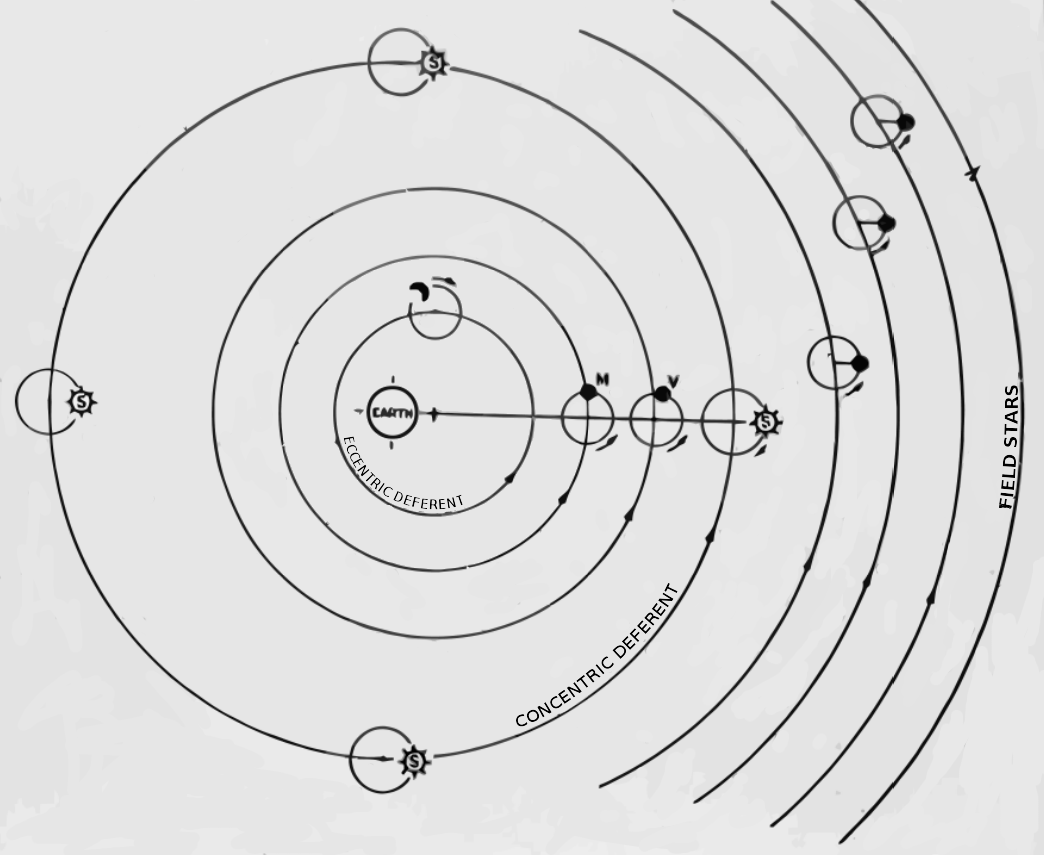
\includegraphics[width=0.45\linewidth]{Figures/0_PtolemaicModel.png}
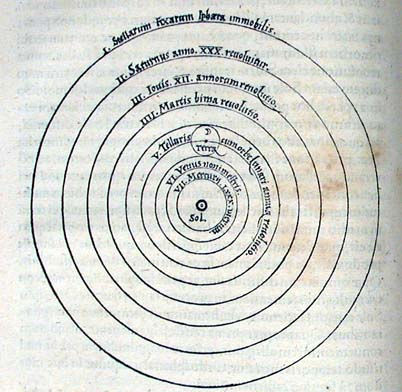
\includegraphics[width=0.38\linewidth]{Figures/0_CopernicusModel.jpg}
\caption{ Left: Depiction of the Ptolemaic geocentric system, the equant is not shown . Right: Copernicus illustration of his own heliocentric system, from \textit{De revolutionibus}. }
\label{Fig:0_PtolemyCopernicus}
\end{figure}



The astronomical evidence was, at the time, paradoxically against him. The apparent size changes of planets could not be measured yet, as well as stars parallaxes, contradicting heliocentrism. The idea of a moving Earth implied some effect on falling bodies (known today as coriolis effect) which were also not measurable at the time. Building on this apparent counter-evidence and on the work of indian astronomer Nilakantha Somayaji, Tycho Brahe, the most renowned astronomer of his time, proposed an alternative model known as the Tychonic system in the late 16th century \citep{ramasubramanian1998}. Brahe maintained the Earth as the center of the universe, circled by the sun, itself orbited by all other planets. The system was very efficient and was quickly adopted by the Church and considered in compliance with the Holy Scriptures.

However, the seed of heliocentrism was planted in european scientific minds. The idea exalted the impetuous and visionnary Giordano Bruno, who pushed the decentralization of Earth to the extreme, claiming stars were other suns, harboring other planets, which themselves could sustain intelligent life. For this, his rejection of catholic dogma and his vehement refusal of retractation, Bruno was burned at the stake on the Campo de Fiori in 1600. Bruno, the fiery dialectist, despised geometry and believed the mind alone could unravel any mystery. 

Johanes Kepler believed in geometry, in consistency and in observations. Ardent supporter of copernicism, he convinced Tycho Brahe to grant him access to his astronomical data, unsurpassed at the time. Focusing on the motion of Mars, Kepler, through trial and error, found out the planet was moving around the Sun following an ellipse. He formulated his first two laws of planetary motions. Further exploration led him to the third law. The three laws of Kepler were formulated, initiating the mathematisation of astronomy, and with it of all physics.

\subsection*{The Starry Messenger}


The father of modern astronomy, and precursor of modern science, Galileo Galilei was born in Pisa in 1564. For the first part of his scientific career, Galileo got famous for his lectures on mechanics and motion. Building on Buridan and Oresme's ideas, he expressed the mathematical form of free fall motion $ d = \frac{gt^2}{2}$. Galileo also formulated what was essentially the future first law of motion from Newton.

In 1609, his passion for scientific instruments led Galileo to build his own "dutch perspective glass", or telescope, a pioneering optical device from the netherlands. Once pointed at the sky, the device triggered an avalanche of observations who would forever bury the aristotelitian view of perfect and unchanged heavens. Moving Jupiter satellites, Moon craters and mountains, millions of stars in the Milky Way, these were consigned into \textit{Sidereus Nuncius} (Starry messenger), the first scientific publication of astronomical observations \citep{galileo1610}.

Strong advocate of copernicism, but lacking proper evidence, Galileo caused a large controversy with his 
\textit{Dialogue Concerning the Two Chief World Systems} published in 1632, a pamphlet against the ptolemaic system, presenting (arguably unintentionnaly) one of its advocates as a simpleton. Despite his friendship with the pope, he had to retract his work and reject copernicism. Galileo spent the rest of his life on house arrest. Observationnal evidence at the time was still on the side of geocentrism, but the extent of the backslash against Galileo showed the febrility of a Church having absorbed Ptolemy and Aristotle principle into its doctrine, in a time where the debate was shifting from theology to physics and observations.

The relativity of motion is often attributed to Galileo, as he includes it in its controversial pamphlet, stating that a traveller inside a ship sailing smoothly would not be able to tell he's moving. Thus, people could be standing on a moving Earth without feeling it. However, this thought experiment was nothing new at the time and had been a recurring theme of mechanical philosophy since Buridan. Oresme, Copernicus and Bruno had been building on the idea, expanding and improving it, developing over the centuries an implicit understanding of inertia, until Bruno actually gives it a name: \textit{virt\`u}. Galileo may have met Bruno himself, and had surely been influenced by his writings \citep{DeAngelis2015}. Galileo's formulation was clearer, and part of a larger understanding of motion, introducing the concept of reference frame. After Copernicus decentralized the Earth, Galileo decentralized human subjectivity itself, setting the scene for the revolution to come. 

\subsection*{On the shoulders of giants}

Isaac Newton is without a doubt the father of modern mathematical science. Admitted in Cambridge in 1661, Newton supplemented the -still- official aristotelitian teaching with more modern authors: Copernicus, Galileo, Kepler, and most of all, Descartes. The french philospher had a profound impact on the young student, rooting his love for mathematics and deductive reasoning. However, while Descartes showed disdain for experimentation, Newton was an acute observer of the natural world. 

In 1666, while in is mother's farm, having been forced out of Cambridge by the Plague, Newton began his reflexion on the motion of celestial bodies. He derived from Kepler's law that the Sun had to exert an inverse squared distance attraction on the planets. Extending the concept to the Earth, moon, and a famous apple, Newton found a way to verify his hypothesis, using data from Galileo mechanical studies on the strength of Earth attraction. The wrong estimate of Earth radius he used at the time introduced a discrepancy which put the young man off his \textit{gravitas} studies for 18 years.

Edmond Halley, astronomer and friend of Newton, having heard of Newton inverse squared law, urged him in 1684 to communicate his work the Royal Society. With a new accurate measure of Earth radius and confronted to a concurrent claim to his law from Robert Hooke \citep{Kramer1982}, Newton capitulated to Halley's eager enthousiasm and communicated his work in the famous \textit{Philosophiæ Naturalis Principia Mathematica} \citep{Newton1687}. Published at Halley's own expense, the Principia shook all of Europe. Newton had invented Calculus (in parallel of Leibniz) and applied it to derive the universal law of Gravitation.

\begin{equation}
F = G \frac{m_1.m_2}{r^2}
\end{equation}


Where:
\begin{itemize}
 \setlength\itemsep{-0.5em}
  \item[$F$] Gravitational attraction between object 1 and object 2
\item[$G$] Gravitational constant, $6.67408.10^{-11} m^3 kg^{-1} s^{-2}$ \citep{Pavese2015}
\item[$m_i$] Masses of object 1 and 2
\item[$r$] Distance between object 1 and 2
\end{itemize}

Though Newton was part of continuous line of geniuses and innovative minds building from each others, as he puts it "If I have seen further it is by standing on the shoulders of giants" \citep{Maury1992}, his input was truly revolutionnary. He made large advances in optics and mathematics, and created a consistent mathematical framework to compute motions, essentially founding modern science and sowing the seeds of the industrial revolution. This framework is summed up by Newton's three laws of motion (from recent translation \citealt{Cohen1999}):

\begin{quote}
Law I : Every body persists in its state of being at rest or of moving uniformly straight forward, except insofar as it is compelled to change its state by force impressed.
\end{quote}

\begin{quote}
Law II: The alteration of motion is ever proportional to the motive force impress'd; and is made in the direction of the right line in which that force is impress'd.
\end{quote}
 
 \begin{quote}
 Law III: To every action there is always opposed an equal reaction: or the mutual actions of two bodies upon each other are always equal, and directed to contrary parts.
 \end{quote}

The second law can be mathematically formulated in more modern terms:

\begin{equation}
\sum \bold{F} = \frac{d \bold{p}}{dt}
\end{equation}

Meaning the sum of all forces $\bold{F}$ applied to an object is equal to the time derivative of its momentum $\bold{p} = m.\bold{v}$.



\subsection*{The n=3 body problem}

As the Enlightenment brought a scientific revolution in many fields, I will now limit the discussion to the development of celestial mechanics, while acknowledging input from other fields.

While the two-body problem had been solved by Newton and expanded by Bernoulli in 1710 \citep{Barrow1997}, in the 18th century the three-body problem remained the object of much investigation and development. A general solution for the Earth-Moon-Sun system would have had applications on nautical astronomy and trans-continental navigation. Extended analytical work by d'Alembert, Clairaut, Euler and Lagrange led to the development of early families of approximate solutions or exact solutions to special cases.

From 1773 to 1793, Joseph-Louis Lagrange, helped by his invention of Lagrangian mechanics, would make a lot of advances on the three-body problem. He introduced the concept of potential and discovered libration points (later known as Lagrange points). In the same time, Pierre-Simon de Laplace proved the stability of the solar system using a newly developped perturbation theory. The solar system dynamics were being unraveled, with finely tuned perturbation computation, but the general three-body problem remained unsolved.

In 1888, Henri Poincaré, greatest mathematician of his time, submitted an entry to a contest organized by the King of Sweden Oskar II. The goal was to determine a usable solution to the n-body problem, for any given n. While Poincaré does not submit a complete solution, he wins the contest by presenting an in-depth exploration of the phase-space of the restricted three-body problem, which would later give rise to the Chaos theory ,see \cite{Yoccoz2010}. Poincaré managed to prove that the three-body problem had no  solution involving simple functions.

Contrary to popular belief, the three-body problem \textit{has} a solution, it was derived by Karl F. Sundman in 1912 \citep{Sundman1912}. However, any attempt to obtain accurate trajectory predictions would face tremendous convergence time and is in practice unusable \citep{Beloriszky1930}.

It is interesting to note that Elis Str\"omgren performed by-hand calculation of a three-body system, see \cite{Aarseth2003,Stromgren1909}, prefiguring the advent of numerical orbit computation.

\subsection*{The n$>$3 body problem}

\begin{quote}
"The Sun attracts Jupiter and the other planets, Jupiter attracts its satellites and similarly the satellites act on one another."
\end{quote}

By this sentence from the \textit{Principia}, Newton formulates the n-body gravitational problem, an arbitrary number of massive bodies all interacting gravitationally, for the solar system. The "n$>$3-body" problem didn't receive a lot of attention at first, as the unruly three-body problem was on everyone's mind, and a n$>$3-body problem seemed abstract, the solar system example being appropriatly dealt in approximations.

In 1764, Charles Messier resolved individual stars in Messier 4, a globular cluster, hundreds of thousands of stars grouped together. Many new clusters were to be found afterwards, extending the catalog of real-life n-body systems. However, nothing was known of their kinematics, the stars were somehow suspended motionless in the sky. This was the case until the advent of Doppler spectroscopy, which allowed astronomer to measure stars velocities \citep{Doppler1842}. Stellar dynamics had begun.

The n$>$3-body problem was still inaccessible, so scientists like James Jeans and Arthur Eddington decided to take the problem from the other hand, and took advantage of the large number of stars. Inspired by \cite{Poincare1906}, both astronomers applied the statistical theory of gas to stellar systems, founding the field of stellar dynamics \citep{Jeans1916,Eddington1916}.

An interesting experiment was conducted by \cite{Holmberg1941} to understand the collision of two stellar systems (galaxies). With too few points to warrant a statistical approach, and before the rise of numerical integration, Holmberg modelled two galaxies with dozens of lightbulbs and photocells, measuring the attractive force with the amount of light received in each direction, taking advantage of the inverse squared fall of luminosity with distance, akin to gravity.

\subsection*{The numerical age}

The first numerical N-body computations were performed by Sebastian Von Hoerner in 1959 when visiting the University of T\"ubingen, on a Siemens 2002, a cutting edge calculator at the time. The very first had N=4. Then, Von Hoerner, back in Heidelberg, worked his way up to 16 stars, then 25, programming and debugging on punch cards. This story was told by Von Hoerner himself in \cite{VonHoerner2001}. He very quickly realized the importance of binary stars and their impact on computations. He was also able to confirm some theoretical prediction on cluster dynamics, and found an interesting radial density profile with a center cusp \citep{VonHoerner1960,VonHoerner1963}.

\begin{figure}
\label{Fig:N_increase}
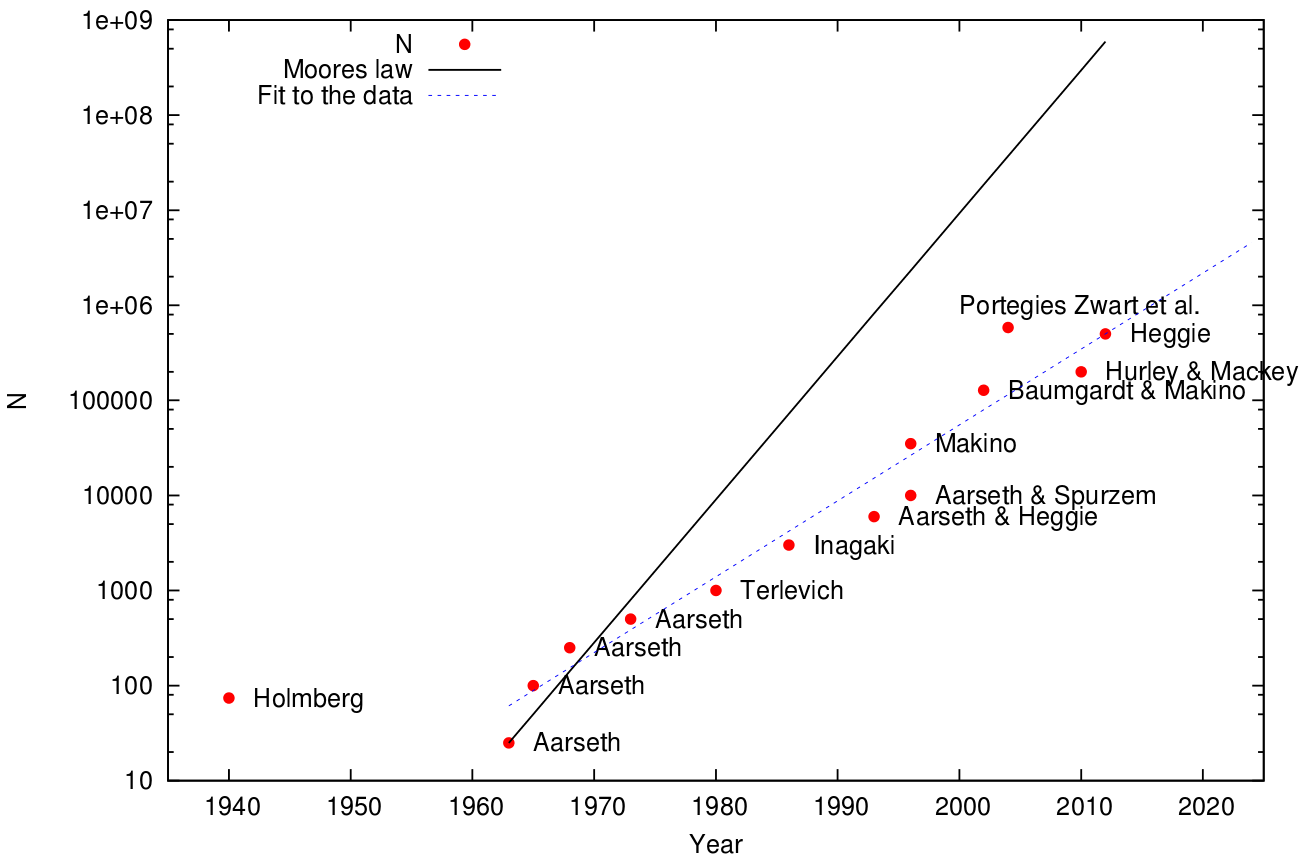
\includegraphics[width=0.9\linewidth]{Figures/0_N_increase.png}
\caption{The evolution of the number of particles in N-body simulations. Solid line shows the Moore law. The figure was taken from \protect\cite{Bedorf2012}. }
\end{figure}


There was two ways to increase the number of stars in simulations: buy a better computer or improve the algorithm. Sverre Aarseth got invested in the second path, which would take over his scientific life. Aarseth pioneered the use of individual time-step, changing the rate at which particles positions are updated, gravitationnal softening, allowing convergence for close approach, and polynomial prediction for force calculations \citep{Aarseth1964}. As power and optimization grew, investigations expanded, such as the interaction star-gas \citep{VanAlbada1968a} and binary formation \citep{VanAlbada1968b}.

The 1970s brought two new important optimisation methods: KS regularization of close pairs \citep{Aarseth1972} and Ahmad-Cohen neighbour scheme \citep{AhmadCohen1973}. The number of stars in simulations kept growing, reaching 1000 with \cite{Terlevich1980} and materializing into the \textit{NBODY5} integrator. At this point various methods departing from a pure collisional calculation began to emerge, such as the simplified distant interaction with the \cite{BarnesHut1986} tree algorithm.

To go beyond the regular improvement of computing power with time, a group of japanese researchers, among whom Junichiro Makino, designed and built special purpose hardware for many-body problems: GRAPE \citep{Ebisuzaki1990,Ito1991}. These cards vastly improved the speed of nbody simulations and were a milestone on the road to the parallelization of computing. With the force calculation directly implemented in the hardware, GRAPE dominated the field for 15 years.

The latest technological leap in Nbody simulations came from graphic cards, see \cite{Bedorf2012} for a more detailed historical perspective. Graphical Processing Units, or GPU, were originally designed for computer games visual rendering, applying the same transformations to a lot of pixels at the same time. These made them very efficient parallel computing machines for physics. Interest in GPU computing started to grew in the 2000s \citep{Nyland2004,Elsen2006,SPZ2007} until the advent of usable GPU programming languages, like CUDA, in the late 2000s. At this point GPU were more efficient than GRAPE hardware for force calculation. Keigo Nitadori and Sverre Aarseth developped a GPU-accelerated version of the latest NBODY code, NBODY6, in 2012 \citep{Nitadori2012}.

Last year, 329 years after the publication of the \textit{Principia}, a collisional nbody simulation of one million stars was performed with a modified version of NBODY6 running on GPU \citep{Wang2015}. Computers have made it possible for humans to study systems of incredible scales in space and time, only using the universal law of gravitation. N-body numerical integrators are the culmination of centuries of scientific development on the motion of massive bodies.



\newpage
\section{Star clusters}

\subsection{What are star clusters ? And why study them ?}

The widest definition possible for a star cluster is "An area of the sky with visibly grouped stars". However, this includes binary stars and galaxies. We are interested in intermediate systems, such as open clusters, globular clusters or associations, in which stars are, if not bound, at least under direct mutual gravitational influence. These objects can either dissolve in less than a million year or remain bound for billions of years.

Clusters are the result of bursts of star formation in Giant Molecular Clouds. All stars within a cluster were born approximately at the same time, which explains the sustained interest of the scientific community for star clusters for more than a century. They are the best laboratories of stellar physics available to us: a large population of stars sharing the same age and distance to Earth. The age of the cluster can be derived from the most massive stars in the population, as stars have lifetimes inversely correlated with their mass. Overall, integrated spectral features from all members of a star cluster can provide a wealth of information.


\begin{figure}
\center
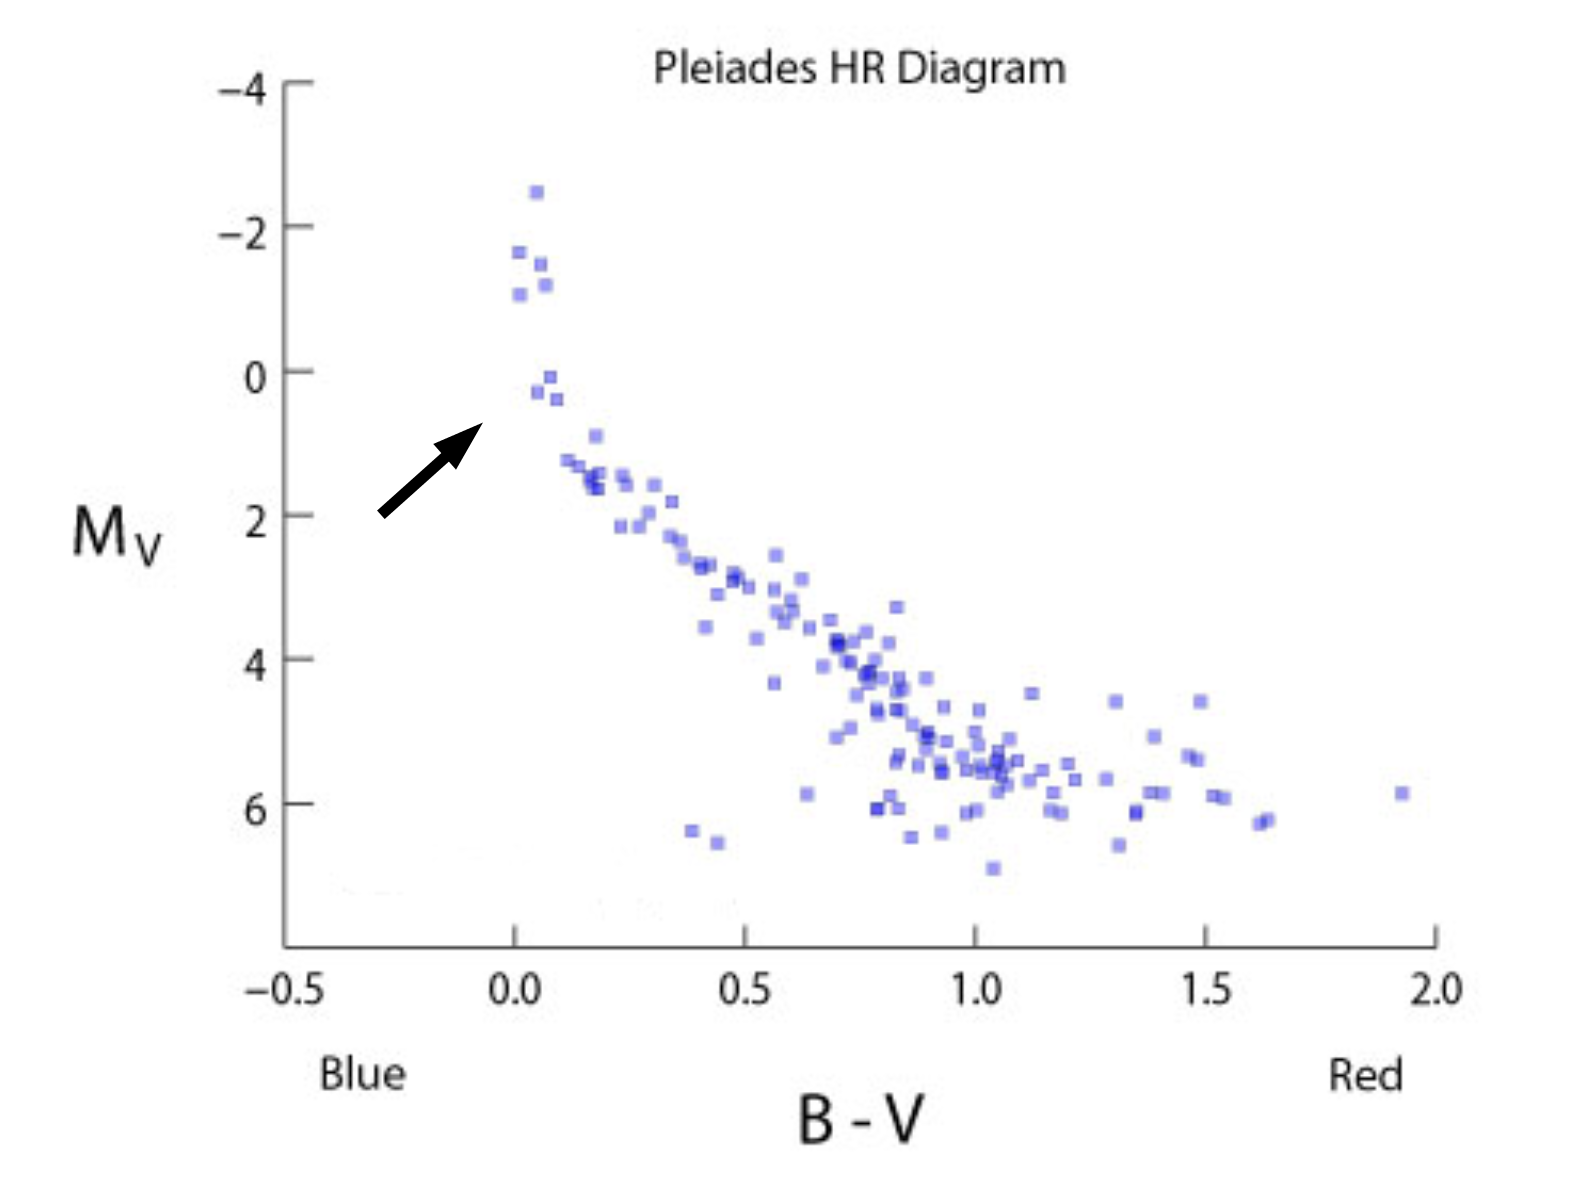
\includegraphics[width=0.45\linewidth]{Figures/0_HRDiagram_Pleiades.png}
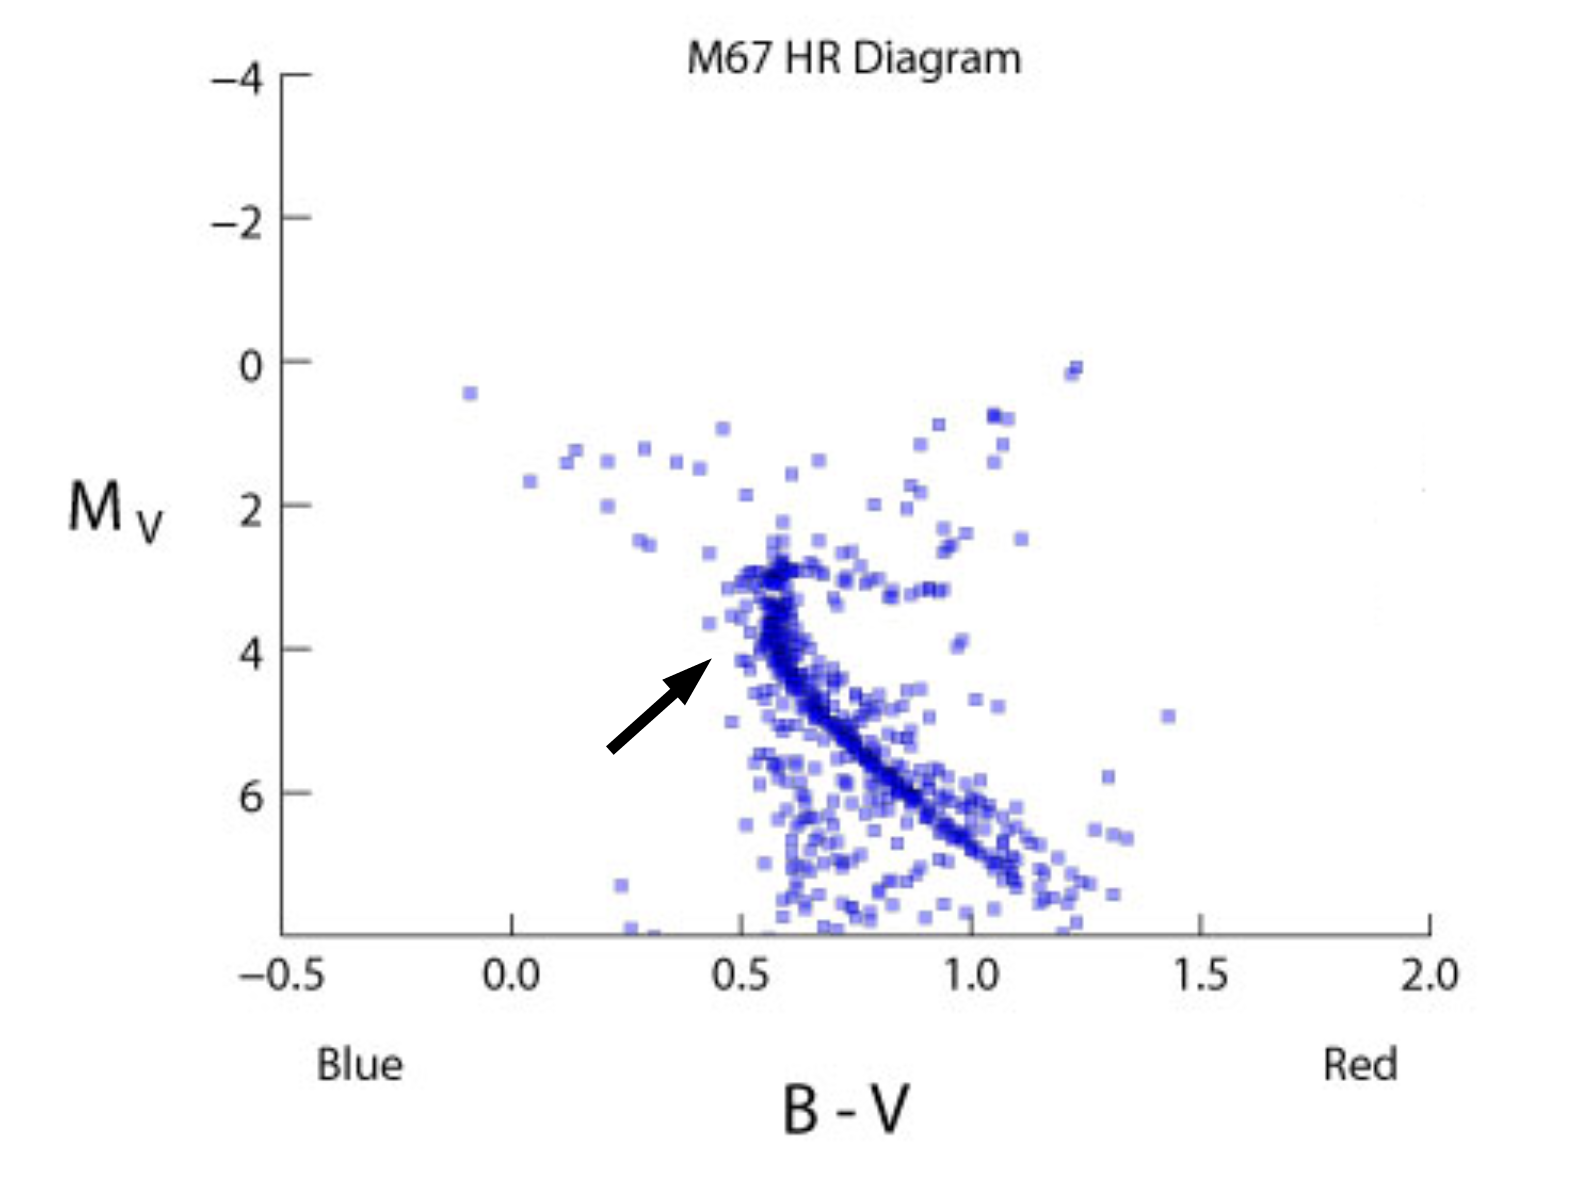
\includegraphics[width=0.45\linewidth]{Figures/0_HRDiagram_M67.png}
\caption{Hertzprung-Russel diagram of the Pleiades and M67. An arrow points at the Main-Sequence turn-off for each cluster. The figures were taken from the \href{http://www.astrophysicsspectator.com/topics/stars/HertzsprungRussellClusters.html}{Astrophysics Spectator} website and data can be found in \protect\cite{Stassun2002,Kharchenko2004}  }
\label{Fig:0_HR}
\end{figure}

One example is the ability to date a cluster, thus its members, through the main-sequence turn off. On figure~\ref{Fig:0_HR} is shown the Hertzprung-Russel diagram for two different clusters: The Pleiades and M67. The HR diagram shows the luminosity of the star versus its color, redder on the right, bluer on the left. Stars spend most of their life on the Main Sequence, with the most massive, luminous blue stars on the left, and red fainter smaller stars on the right. Massive stars have shorter lives and depart from the main sequence before small stars. Looking at the Main Sequence turn-off in the HR diagram of a cluster tells us the mass of the stars currently leaving the MS, which gives its age and that of all other stars. As seen on the figure, the Pleiades are younger (100Myr) than M67 ($\sim$ 4 Gyr) as the stars leaving the MS are more massive.

Star clusters are historically divided into two main categories: globular clusters and open clusters. As observationnal techniques improve, categories tends to blend into a spectrum of size, age, and dynamical state, with Young Massive Clusters, embedded clusters, associations.






\subsubsection*{Globular clusters}

Globular clusters are old and massive stellar systems. Most of them are older than 10 Gyr and more massive than $10^4~M_\odot$. They only contain stars, with no dust or gas. The 150 known globular clusters in the Milky way are scattered in the disk and the halo. Due to their age, GCs are dynamically evolved. Introducing the relaxation time, defined in \cite{BT} by:
\begin{equation}
\label{Eq:0_relaxation}
t_{relax} = 0.1 \frac{N}{logN} t_{cross} = 0.1 \frac{N}{logN} \frac{R_{hm}}{\sigma}
\end{equation}

with $t_{cross}$ the crossing time, defining the time a star takes to cross the system and $\sigma$ the internal velocity dispersion. The relaxation time is the time it takes for a system to erase its initial condition, perturbation per perturbation. GCs have a relaxation time of about a Gyr, they are relaxed systems. Various models have been put forward for the structure of GCs, the King \citep{King1966} and Plummer \citep{Plummer1911} models are the most widely used.




\begin{itemize}

\item 47 Tucanae (NGC 104) is one of the most massive known globular cluster in the Milky Way. It is estimated to contain about 1.5.$10^6~\Mo$ and to be 13 Gyr old\citep{Forbes2010}. Its core is extremely dense, as many GCs, with a central density up to $10^6 \Mo/\textrm{pc}^3$. Such a concentration of stars is a favorable environment for stellar collisions, which create what is called \textit{stellar exoticae}, stellar object not following the standard evolutionnary path, such as blue stragglers. Blue stragglers are stars too luminous and too massive compared to the age of the cluster, likely formed out of colliding stars. 47 Tuc exhibits a population of such objects, as well as others: Cataclysmic variables, X-ray binaries, etc. These are the direct consequence of the very dense environment of globular clusters such as 47 Tuc.

\item Messier 12 (NGC 6218) is on the light end of the mass spectrum with 9.$10^4~\Mo$ \citep{Marks2010}. Such a low mass is however thought to be due to the cluster's dynamical history. Globular clusters have orbits around the galaxy, some more dangerous than others. For example Palomar 5 is currently disappearing after violent encounters with the galactic center. A study by \cite{DeMarchi2006} showed M12's orbit probably also passes close to the galactic center. Subjected to the strong tidal forces of the galactic bulge, M12 would have lost about 4/5 of its original mass. This scenario is backed by the mass function of M12. The mass function is the distribution of stellar masses, and its slope is thought to be more or less universal, though it appears unusually flat in M12. The tidal shock would have preferentially depleted low mass stars, as a process known as mass segregation tends to have massive stars sink at the center and low-mass stars overpopulate the outskirts of the system. 

\item NGC 2808 is reported to contain 1.4 $10^6~\Mo$ \citep{Boyles2011}. NGC 2808, as all others GCs, had long been thought to have an homogeneous stellar population. Yet, a study by \cite{Piotto2007} showed NGC 2808 contained at least three different stellar sequences. As this cannot be explained by the natural age spread arising from a continuous star formation at the birth of the cluster, such observations have far-reaching implication on its formation scenario, and those of many GCs with multiple populations. Several hypothesis are being explored, such as GCs being the outcome of mergers \citep{Pasquato2016} or a sequence of distinct star forming events \citep{Dantona2016}, with no consensus for now.

\end{itemize}


\begin{figure}
\label{Fig:0_GlobularClusters}
\center
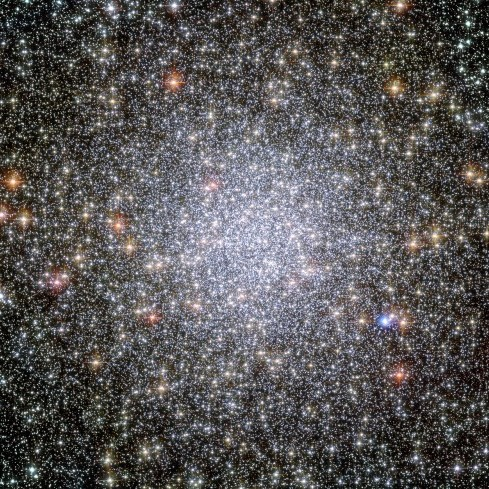
\includegraphics[width=0.3\linewidth]{Figures/0_47Tuc.jpg}
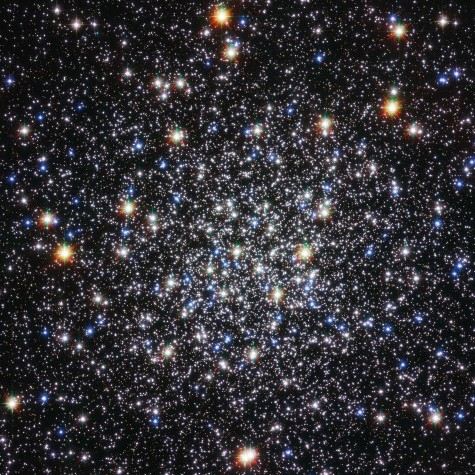
\includegraphics[width=0.3\linewidth]{Figures/0_M12.jpg}
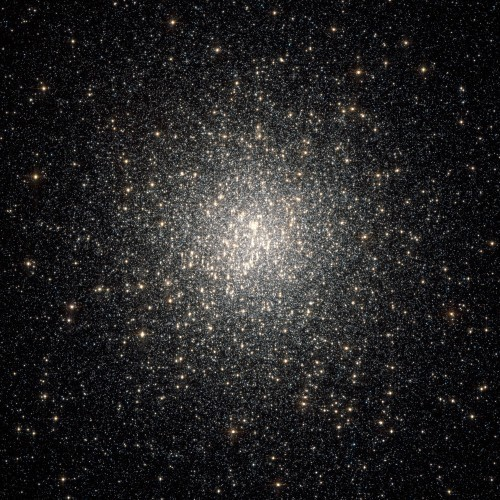
\includegraphics[width=0.3\linewidth]{Figures/0_NGC2808.jpg}
\caption{From left to right: 47 Tucanae, Messier 12 and NGC 2808. Credits: ESA/Hubble. }
\end{figure} 


\subsubsection*{Open clusters}


\begin{figure}
\center
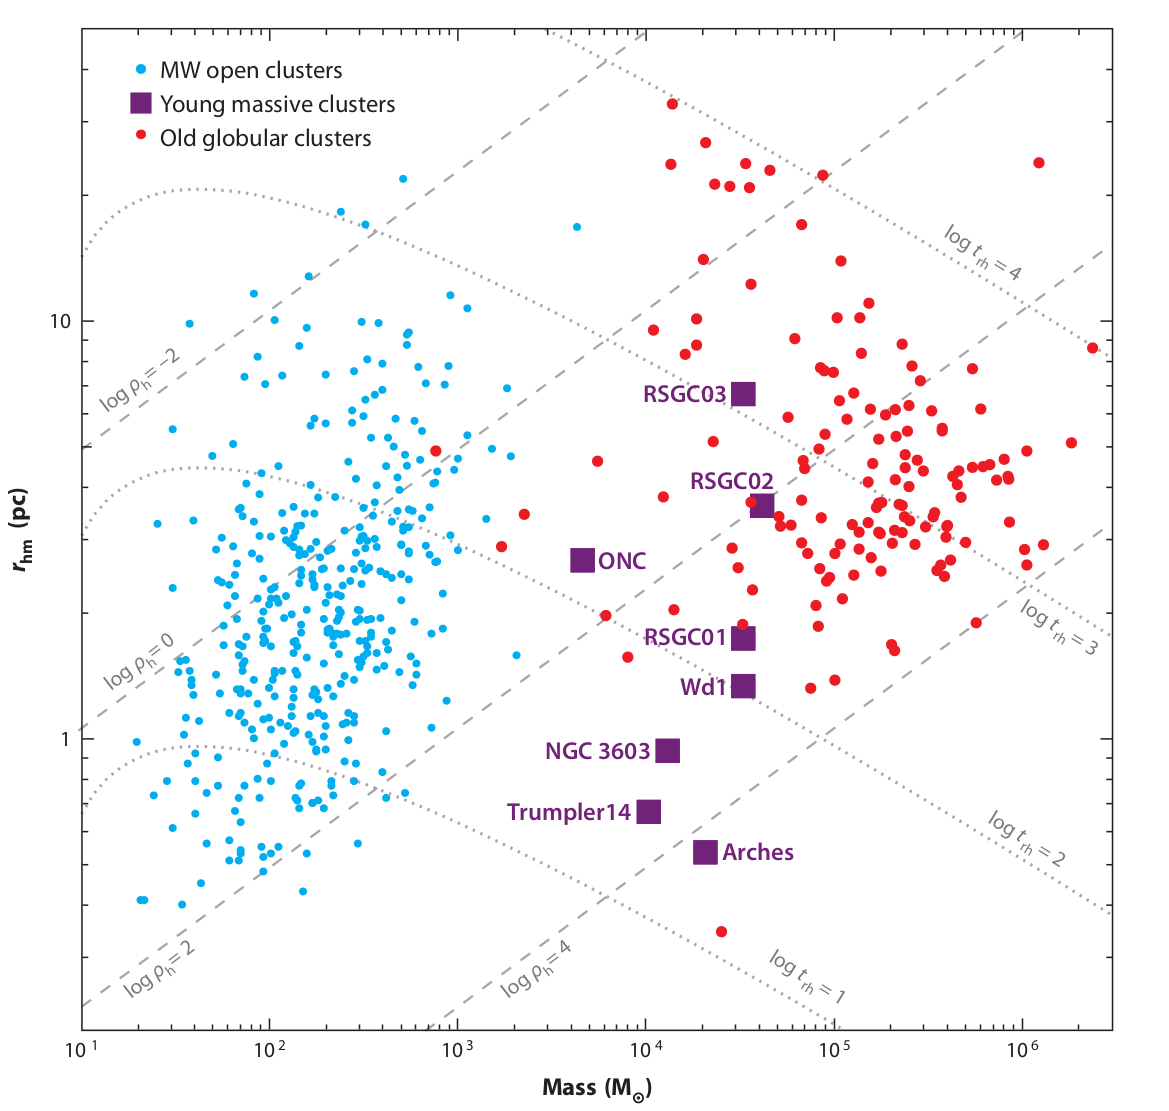
\includegraphics[width=0.65\linewidth]{Figures/0_MassRadiusClusters.png}
\caption{Radius-Mass Diagram for Milky Way clusters. Blue dots are open clusters, red dots Globular clusters and purple squares show Young Massive Clusters. Dashed lines show constant density within half-mass radius $\rho_h = 3M/8\pi r^3_{hm}$ and dotted lines show constant relaxation time. The plot was taken from the review \protect\cite{PortegiesZwart2010}.}
\label{Fig:0_SPZ}
\end{figure}


Open clusters are lighter objects, rarely more massive than $10^3 \Mo$. They are also younger, typically no older than a Gyr. In fact, Open Clusters are thought to be very volatile, with the vast majority not surviving beyond 100Myr. Causes of disruption include internal two-body evolution and tidal shocks from passing massive clouds on nearby orbits.



\subsection{Formation in Giant Molecular Clouds}

\subsection{Early dynamical evolution}

\subsection{Binary stars in clusters}









\newpage
\section{NBODY6}


NBODY6 is the second youngest iteration of the NBODY family, a suite of n-body integrators created by Sverre Aarseth. It can compute the gravitational interaction between up to 128,000 stars in a collisional fashion, meaning there is no softening of the potential, at any scale. This allows for very close binaries to form and remain in the system. To achieve its impressive performances, NBODY6 relies on several optimization technique which have been first developed in the 1960s and 1970s, and improved ever since. Here will be developped four major features of NBODY6, in chronological order of their implementation: block time-step, KS-regularization, Hermite scheme and Ahmad-Cohen neighbour scheme. A full description can be found in Sverre Aarseth's book \citep{Aarseth2003}.% Inspiration for this section should be credited to the user manual of NBODY6++, written by Emil Khalisi and Rainer Spurzem.

\subsection{Block time-step}
 
In the first Nbody simulations, the system was integrated with an universal time-step, determined by the most accelerated star. A star in the outer regions of the cluster with a small velocity did not need to be updated that often. One of the first improvement  was the introduction of individual time-step: each star is attributed its own time-step, depending on the force that is applied to it and its derivative:

\begin{equation}
\Delta t_i =  \eta \sqrt{\frac{ |\bold{F_i}||\bold{F^{(2)}_i}| + |\bold{F^{(1)}_i}|^2 }{|\bold{F^{(1)}_i}||\bold{F^{(3)}_i}| + |\bold{F^{(2)}_i}|^2}}
\end{equation}
 
With $\bold{F}^{(j)}_i$ begin the j-th derivative of the force applied to particle i and $\eta$ a user-defined accuracy parameter. Such a complex formulation is the result of extensive tests and is quite robust for many special cases. Individual time-steps leads to desynchronized particles, hence the need to interpolate the positions of other particles to compute $\bold{F}_i$, which was achieved through fourth-order polynoms.
 
 To limit the amount of desynchronization, block-time steps were introduced. Instead of having as many time steps as particles, one only allows quantized power of 2 of an initial time step. $\Delta t_0$,$\frac{\Delta t_0}{2}$, $\frac{\Delta t_0}{4}$, $\frac{\Delta t_0}{2^i}$. All time steps are then commensurate and regularly fall back on the same time steps, minimizing the amount of interpolation during the force calculations.
 
\begin{figure}
\label{Fig:blocktimesteps}
\center
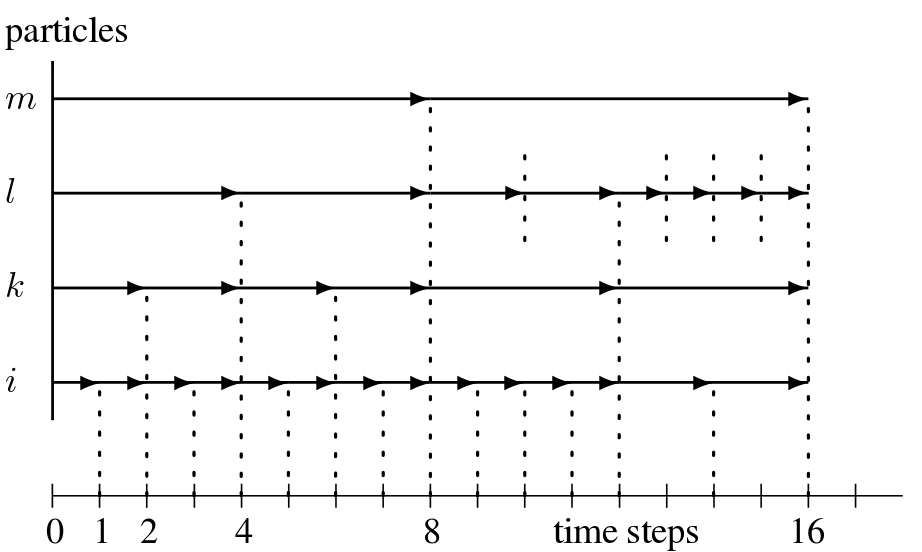
\includegraphics[width=0.6\linewidth]{Figures/0_block_timesteps.png}
\caption{Illustration of block time steps on 4 particles. Particles get their positions updated for each arrow symbol, common time steps are shown as vertical dotted lines. Figure from NB6++ User Manual. }
\end{figure} 
 
 
\subsection{KS-regularization}



\subsection{Hermite prediction scheme}

\subsection{Ahmad-Cohen neighbour scheme}




\newpage
 \section{Young star clusters}












    
%    \pagestyle{main}
%      % partie 1
%    \part{Contexte physique et médical}
%    \label{Part1}
    %%%%%%%%%%%%%%%%%%%%%%%%%%%%%%%%%%%%%%%%%%%%
% Chapitre 1
%%%%%%%%%%%%%%%%%%%%%%%%%%%%%%%%%%%%%%%%%%%%

\chapter{The Hubble-Lema\^itre fragmented model} 
\label{ChapterHL}

\section{How to build a Hubble-Lema\^itre model}

\subsection{Initial state}

The first step to obtain a HL-fragmented model is to build an uniform sphere model. The N stars, depending on the required membership, have to be distributed randomly in space inside a certain radius, producing an uniform density. This can be achieved by sampling separately the distance to the center and the angular position of each star, in a method analog as used in \cite{Aarseth1974} for a Plummer model. The distance to the center should be sampled from the function:

\begin{equation}
f_R(X) = R_0 X^2
\end{equation} 

With $R_0$ the bouding radius and X a random variable following a uniform probability law between 0 and 1. A direct uniform law for the radius would overpopulate the outer regions. The angles $\phi$ and $\theta$, respectively azimuthal and polar angle in the physics convention, should be sampled from:


\begin{align}
f_\phi(X_1) & = 2\pi X_1\\
f_\theta(X_2) &= \arccos{ (X_2) }
\end{align}

With $X_1$ following a uniform probability law between 0 and 1 and $X_2$ between -1 and 1. The cartesian coordinates are then found:

\begin{align}
x &= R \sin{\theta} \cos{\phi}\\
y &= R \sin{\theta} \sin{\phi}\\
z &= R \cos{\theta} \\
\end{align}

The N particles are then homogeneously distributed in space in a sphere of radius $R_0$. The next step is to attribute velocities. Unlike other models like the Plummer model, the velocities are here straightforward. We use the well known velocity field of neighbouring galaxies: velocities are radial from the Milky Way, larger with increasing distances, taking the form:

\begin{equation}
\label{Eq:1_Hubble}
\bold{v} =  \textrm{H}_0 \bold{r},
\end{equation}

with H$_0$ being an equivalent of the well-known Hubble parameter. For historical accuracy, I added the name of Georges Lema\^itre when I named my model. It has now been shown that the astronomical observations of redshifted galaxies and its interpretation as the consequence of an expanding universe predated Hubble's paper \citep{Hubble1929}. Georges Lema\^itre had published his conclusion on an expanding universe two years earlier \citep{Lemaitre1927}. The account of this can be found in \cite{Kragh2003,VanDenBergh2011} and \cite{Freeman2015}.

An appropriate H$_0$ to obtain a fragmented subvirial model has to be inferior to 1.4 (see next section). The model obtained from this is then evolved through a nbody integrator, which in my case is NBODY6.


\subsection{Fragmentation}

The cluster expands, driven by the initial Hubble-Lema\^itre velocity field. During this expansion, poissonian fluctuation in density from the uniform model starts to grow: the part of the cluster with more mass initially attract more stars, forming clumps, clumps merge, spontaneously building substructure. These clumps will be analyzed in another section. If H$_0$ is well chosen, the expansion stops at some point, the apex, at which the initial kinetic energy has been spent and converted to potential energy: the cluster is now larger, substructured and subvirial, about to collapse. The apex time $t_a$ of the end of the expansion and the critical value of H$_0$ can be derived from Newton's second law applied to an expanding spherical shell of matter.

We start from a uniform sphere of radius $R_0$, total mass $M$. We consider spherical shells as mass elements, situated at distance $r$ from the origin. As previously said, they are attributed a radial velocity following (for the shell at $r=R_0$) $\vec v_0 = \Hub_0 \vec R_0 = \Hub_0 R_0 \vec u_r$. We want to follow the radial motion of the last shell of mass m, situated at $R$ from the origin. Newton's second law gives:


%\begin{equation}
\begin{align}\label{eq:newton}
m \frac{dv}{dt} & = - \frac{G M m}{R^2}
\end{align}
%\end{equation}

By multiplying on both sides by $v$ and integrating between a given time and $t=0$, one finds:

\begin{equation}
v^2(t) - v^2_0 = 2GM \left( \inv{R} - \inv{R_0} \right)
\end{equation}

Which becomes, by taking $\nu = v/v0$,  $x= R/R0$ and defining:

\begin{equation}
\label{Eq:1_Estar}
E_\ast = \frac{2GM}{R_0 v_0^2}
\end{equation}
which is a dimensionless measure of the total energy of the system:

\begin{equation}
\nu^2  = 1 + E_\ast \left( \inv{x} - 1 \right) .
\end{equation}

The evolution of the system has 3 outcomes, depending on the value of $E_\ast$:
\begin{itemize}
\item $E_\ast<1$ The velocity is always strictly positive as the system expands ($x->\infty$). The system is unbound.
\item $E_\ast=1$ The velocity approaches zero as the system expands. The expansion "stops at an infinite radius". The system is marginally bound.
\item $E_\ast>1$ The velocity reaches zero for a finite radius, the system is bound and will collapses back on itself once the expansion stops. 
\end{itemize}

Using H\'enon units, $G=1$ and $M=1$, and we choose $R_0$=1. Which gives a critical value $E_*$ to have a bound system: $E_* = \frac{2}{\Hub^2_0} < 1$. This means to have a bound system, which stops expanding at some point, one must have $\Hub_0 < \sqrt{2}$.
We only consider in the following the case in which $E_\ast<1$. We have the expression

\begin{equation}
\nu = \sqrt{1+E_\ast\left(\inv{x} - 1\right)}
\end{equation}

Taking the time derivative gives:

\begin{equation}
\frac{d \nu}{dt} = - \frac{E_\ast}{2 x^2} \left[ 1 + E_\ast\left(\inv{x} -1\right)\right]^{-\frac{1}{2}} \frac{dx}{dt}
\end{equation}

Combining this with (\ref{eq:newton}), one obtains:

\begin{equation}
\frac{dx}{dt} = \Hub_0 \sqrt{1+ E_\ast\left( \inv{x} -1\right)}
\end{equation}

which can be rewritten, using $\tilde{\Hub_0} = \Hub_0 \sqrt{E_\ast-1}$ and $x_t=\frac{E_\ast}{E_\ast-1}$

\begin{equation}
\frac{dx}{dt} = \tilde{\Hub_0} \sqrt{\frac{x_t}{x}-1}
\end{equation}

$x_a$ being the extent of the maximum expansion as we assumed a bound system. The subscript a is for apex. If we choose the notation $u = \frac{x}{x_a}$:

\begin{equation}
\sqrt{\frac{u}{u-1}} \frac{du}{dt} = \frac{\tilde{\Hub_0}}{x_a}
\end{equation}

We know that $x$ varies from 1 to $x_a$, thus $u$ varies from $1/x_a$ to 1. We can then make the change of variable $u = \sin^2\theta$ and separate the variables:

\begin{equation}
\sqrt{\frac{\sin^2\theta}{1-\sin^2\theta}} 2 \sin\theta \cos\theta d \theta = \frac{\tilde{\Hub_0}}{x_a} dt
\end{equation}

which becomes after simplifications:

\begin{equation}
\label{Eq:1_integrand_theta}
[ 1 - \cos(2\theta)]d\theta = \frac{\tilde{\Hub_0}}{x_a} dt .
\end{equation}


We now integrate the expression from $t=0$ to $t$, the time at which the expansions stops and $x$ reaches $x_a$ (wich implies $u_a = 1$ and $\theta_a = \pi /2)$:

\begin{align}
\int^{\pi/2}_{\theta_0} [ 1 - \cos(2\theta)]d\theta  & = \int^t_0 \frac{\tilde{\Hub_0}}{x_a} dt\\
\frac{\pi}{2} - \theta_0 + \frac{\sin(2\theta_0)}{2} & =  \frac{\tilde{\Hub_0}}{x_a} t\\
\pi - 2 \theta_0 + \frac{2}{\sqrt{x_a}}\sqrt{1-\inv{x_a}} & = 2 \frac{\tilde{\Hub_0}}{x_a} t 
\end{align}

which boils down to the expression of the time at which the expansion stops:

\begin{equation}
t_a = \frac{E_\ast \left(\frac{\pi}{2} - \theta_0\right) + \sqrt{E_\ast-1}}{\Hub_0 (E_\ast-1)^{-\frac{3}{2}}}.
\end{equation}

Recalling the quantities:
\begin{align}
E_\ast = \frac{2GM}{R_0 v_0^2}        &;  & x_a=\frac{E_\ast}{E_\ast-1}  &;  &\theta_0 = \sin^{-1}\left(\inv{\sqrt{x_a}}\right)  
\end{align}

See figure \ref{Fig:apextime} for the value of $t_a$ as a function of \Hub$_0$

\begin{figure}
\center
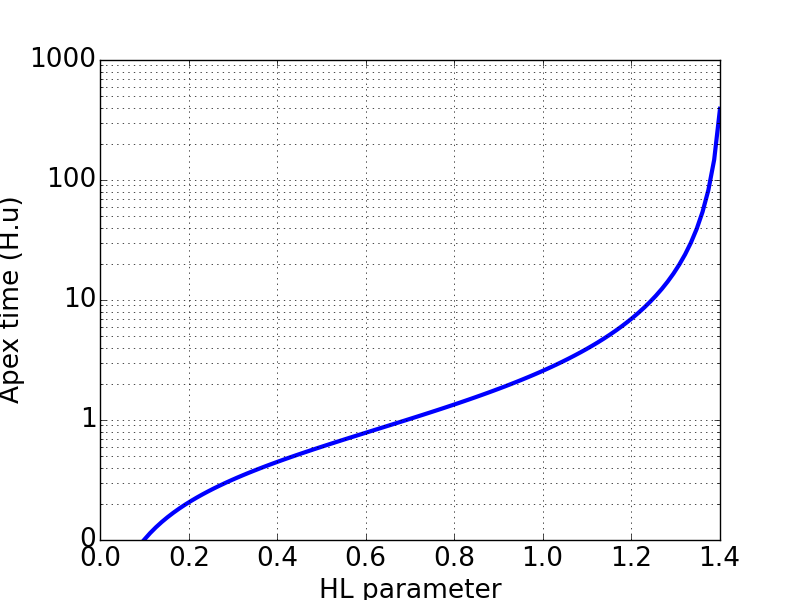
\includegraphics[width=0.7\linewidth]{Figures/1_apextime.png}
\caption{Theoretical values of the apex time, at which the system stops expanding, as a function of initial HL parameter, which tunes the strength of the initial expansion.}
\label{Fig:apextime}
\end{figure} 





\section{The growth of overdensities: analytical study}



\subsection{Working equations}



\begin{table}
\begin{center}
\caption{Summary of main variables.}
\label{Tab:identities}
\begin{tabularx}{\columnwidth}{rl}
\hline
$E$ & Total system energy \\
$E_*$ & Dimensionless total energy \\
$W$ & Total potential energy \\
$E_k$ & Total kinetic energy\\
$\cal M$ & Total system mass\\
$R_o$ & Initial bouding radius\\
$\Hub_0$ & Initial Hubble parameter\\
$v_o$ & Initial velocity at bounding radius\\
$\Hub$ & Variable Hubble parameter\\
$\tau$ & Dimensionless time\\
$x$ & Comoving spatial coordinate\\
$a(t)$ & Rescaling function\\
$\theta$ & Calculation angle\\
$\nu(\tau)$ & Dimensionless velocity $1 + E_*(1/a(\tau)-1)$\\
$\xi$ & Radial displacement from comoving \\
$\delta\rho,\delta M,\delta\rho$ & Perturbed quantities\\
$\mu(\tau)$ & Central point mass\\
$\eta$ & Peculiar velocity $d\xi/dt$\\
\hline
\end{tabularx}
\end{center}
\end{table}

During the expansion and in the mean-field approximation, the mass inside any shell of radius $r(t)$ is conserved as they move outwards. The position of a mass element is known in parametric form from a rescaling of its initial coordinates and we may write 

\begin{align} 
\bold{r}(t) &= a(t)\bold{x}\\
\bold{v}(t) &= \dot{a}\bold{x} = \Hub(t)\bold{r} 
\end{align} 

 where $\bold{x}$ is a co-moving coordinate of position, and $a(t)$ is a dimensionless function of time. The flow is homological and no shell-crossing takes place. It is convenient to introduce a dimensionless time $\tau$ such that 
 
 \begin{equation} 
 \label{Eq:1_taudef}
  t = \frac{\tau}{\Hub_0}.
 \end{equation} 
 
  We then have from equation (\ref{Eq:1_integrand_theta}):
\begin{equation}
\label{Eq:1_Expansion} 
\left. \left[ \frac{ E_\ast}{E_\ast -1} \right]^{\frac{3}{2}} \, \left[ 2\theta - \sin{2\theta} \right]\, \right\vert_{\theta_o}^\theta =  2\sqrt{E_\ast} \tau 
\end{equation}
with 

\begin{equation}  
\label{Eq:1_atheta} 
		a(t)  \equiv  \frac{\sin^2\theta(\tau)} {\sin^2\theta_o}  
\end{equation}


The dimensionless energy parameter $E_\ast$ satisfies  $E_\ast  > 1$ for bound systems. The origin of time $\tau = 0 $ coincides with  the angle $\theta_o$ found from solving 
 $\sin^2\theta_o = (E_\ast - 1) /  E_\ast $. 
%% With $R_o$ and $\Hub_0^{-1}$ dimensional constants for the scales of length and time, repectively, 
The solution (\ref{Eq:1_Expansion})  
provides the time-sequence for the position and velocity of any shell $ 0 < x < R_o$ as parametric functions of $\tau$~: 

\begin{subequations}
\label{Eq:1_HubbleExpr} 
\begin{equation}
 v(t) = \Hub_0 x  \sqrt{ 1 + E_\ast \left( \frac{1}{a(\tau)} - 1 \right) } = \Hub_0 ~ x ~\nu(\tau)
 \end{equation} 
 \begin{equation} 
  \Hub(t) = \Hub_0 ~ \frac{\nu(\tau)}{a(\tau)} 
 \end{equation} 
\begin{equation}
\rho(t) = \frac{3\Mtot}{4\pi R_o^3}\frac{1}{a^3(\tau)}\ . 
\end{equation}			
\end{subequations}

 
\subsection{Linear density perturbation}
\label{Sub:1_FragmentationModes}
An actual Hubble-Lema\^itre model will develop 3-dimensional clumps during the expansion, but to get an analytic view of this process, it is necessary to fall back on one dimension. This will shed light on the growth of clumps and help understand general trends in the system.

We follow radial density perturbations in the expanding uniform sphere described by equations (\ref{Eq:1_Expansion}) and (\ref{Eq:1_atheta}), as the local density increase also gauges the rise in velocity dispersion. A simplified calculation for radial modes of perturbation in the linear approximation will be derived here, with the goal to determine when the clumps become mostly self-gravitating. A more detailed analysis can be found in the classic work by \cite{Friedman1978}, \cite{Peebles1980} and \cite{Aarseth1988} .

We introduce a Lagrangian perturbation in the position of a shell of constant mass by substituting $\mathbf{x} \rightarrow \mathbf{x} + \boldsymbol\xi(\mathbf{x},t)$ and we set $\boldsymbol\xi = \xi \bold{u_r}$ for a radial displacement. A linear treatment of the continuity equation yields an expression for the perturbed density. Starting from the well known equation

\begin{equation}
\frac{\partial \rho}{\partial t} + \nabla(\rho \bold{v}) = 0 
\end{equation}

which transforms into

\begin{equation}
\delta \rho + \nabla (\rho \bold{v} \delta t) = 0.
\end{equation}

We make use of the equivalence:
\begin{equation}
\label{Eq:1_derivequiv}
\frac{\partial}{\partial r} \equiv \frac{1}{a} \frac{\partial}{\partial x}
\end{equation}
to obtain, considering $ \bold{v} \delta t = \delta \bold{r} = a(\tau) \boldsymbol\xi$ and ignoring second order terms from $\delta \rho$:

\begin{equation} 
\label{Eq:1_DeltaRho} 
\delrho = - \mathbf{\nabla}\cdot (a\rho\mathbf{\xi}) =  - \rho(\tau) \frac{1}{x^2}\frac{\partial}{\partial x} ( x^2\xi ) 
\end{equation}

which leads to a perturbation in  the mass integrated up to  radius $r$ 

\begin{align}
\delta M(<r) &= \delta \left( \rho \frac{4}{3} \pi r^3 \right)\\
    &= - 4\pi a^3(\tau) \rho x^2 \xi . 
\end{align}
Poisson's equation in spherical symmetry gives the perturbed potential 

\begin{equation} 
\label{Eq:1_Poisson} 
\frac{1}{r^2}\frac{\partial}{\partial r} r^2\frac{\partial}{\partial r} \delphi =\frac{1}{a^2}\frac{1}{x^2}\frac{\partial}{\partial x} x^2\frac{\partial}{\partial x} \delphi  = 4\pi G\delrho .
\end{equation}
Substituting for $\delrho$ from (\ref{Eq:1_DeltaRho}) in (\ref{Eq:1_Poisson}), and using (\ref{Eq:1_derivequiv}), we obtain:
\begin{equation}
\frac{\partial}{\partial x} \left( x^2 \frac{\partial \delphi}{\partial x} \right) = - 4\pi a^2 G \rho_0 \frac{\partial}{\partial x} \left( x^2 \xi \right)
\end{equation}
Integrating once, we obtain the general solution
\begin{equation}
\label{Eq:1_Gradpsi} 
a(\tau)\nabla \delphi = \frac{3G\Mtot}{R_o^3} \left( - \xi + R_o^3\frac{\mu(\tau)}{x^2} \right) 
\end{equation}
where $\mu$ stands for a central point mass. A point mass would form by shell crossing at the center of coordinates. In an expanding system, shell crossing at the center is unlikely. For that reason, we make $ \mu = 0$ in the remainder of this paper.

The equations of motion at co-moving radius $x +\xi(x,t)$ can be expanded to first order in $\xi$~; identifying terms of the same order we obtain (with $\partial/\partial x = \nabla_x$)

\begin{equation} 
a(\tau) \frac{d^2}{d t^2} \xi + 2 \dot{a}(\tau) \frac{d}{dt}\xi = - \nabla\delphi - \xi \nabla_x \nabla\phi - \ddot{a}(\tau)\xi \ . 
\end{equation} 
The second and third terms on the right-hand side cancel out exactly~; the first is known from (\ref{Eq:1_Gradpsi}). 
It is standard practice to demote this second-order dynamical equation to a set of first order equations~; for convenience we use the initial system radius $R_o$ as unit of length,  and we introduce starred ($\ast$) dimensionless variables. We then have $x = R_o x_\ast, \xi = R_o\xistar$, and so on.  After simplification using the dimensionless functions of $\tau$  defined in (\ref{Eq:1_taudef}) and recalling that $\dot{a}(\tau) = \textrm{H}(\tau)$, the differential equations read

\begin{subequations}
 \label{Eq:1_system}
    \begin{align}
    	\label{Eq:1_systema}
		\frac{d}{d\tau} \xistar &=  \etastar(\tau)  \\ 
		\label{Eq:1_systemb}
		\frac{d}{d\tau} \etastar &= \frac{3 \Estar}{a(\tau)^2}\,\xistar - 2 		\frac{\textrm{H}(\tau)}{a(\tau)} \etastar   
	\end{align}
\end{subequations}
where we have introduced the peculiar velocity $\eta \equiv d\xi/dt = \Hub_0R_o \eta_\ast$.  


\subsection{Consistent initial conditions} 
\subsubsection{Initial conditions} 
Equations (\ref{Eq:1_system}) can be numerically integrated with an explicit integration scheme once the initial values $R_o, \Hub_0, {\cal M}$ and $\xistar(0)$ are specified and values of $a(\tau)$ are obtained from (\ref{Eq:1_atheta}) and (\ref{Eq:1_Expansion}). All functions of the dimensionless time $\tau$ are set to unity except that $\etastar(0) = 0$. The solution is shown on Fig~\ref{Fig:1_tau_ms}.


The Hubble parameter $\Hub(\tau) \rightarrow 0$ when the system reaches a maximum radius $a(\tau)R_o$ ($\theta[\tau] = \pi/2$ in Eq.~\ref{Eq:1_atheta}). Around that time, equation (\ref{Eq:1_systemb}) transforms so the Lagrangian displacement $\xistar$ grows exponentially, and the clumps become the densest. We investigate the growth of a density perturbation as a Fourier fragmentation mode before that. In the linear regime, such a mode is decoupled from all the others. We pick 

 \begin{figure}
	\center
 	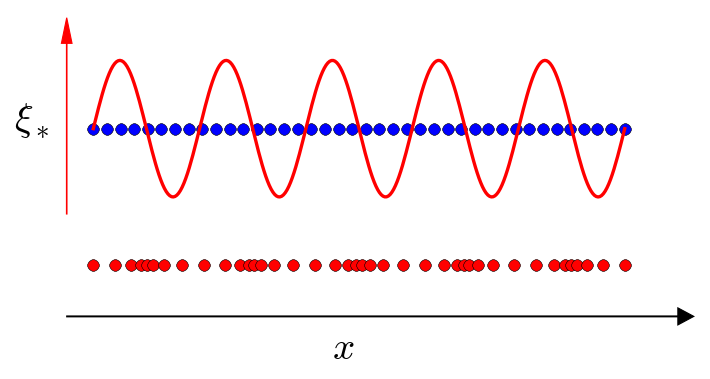
\includegraphics[width=0.7\textwidth]{Figures/1_perturbation.png}
	\caption{Schematic illustration of a sinewave density perturbation (red line) applied to an uniform distribution of matter (blue dots) and the resulting distribution (red dots). The mode displayed here has $m=10$ and its amplitude was exaggerated.} 
	\label{Fig:1_perturbation}
\end{figure}

\begin{equation} 
\label{Eq:1_FourierMode} 
   \xistar(x,0) = \xistaro \sin( kx ) ,
\end{equation}  
where the wavenumber $k$ is such that $k R_o = m \pi$ and $\xistar(R_o,0) = \xistar(R_o,\tau) = 0$ at all times. When deciding which wavenumber to choose, we must bear in mind the finite numerical resolution of the models that we will present later. The next subsection gives quantitative arguments that motivated our choices.  
The aspect of the perturbed system is shown as a rough schematic on Fig~\ref{Fig:1_perturbation}.

\subsubsection{Fourier modes: resolution issues} 
\label{Ssub:1_FourierModes}
An uniform distribution of $N$ discrete mass elements cannot resolve infinitely small wavelengths, the lower limit depends on the mean separation $l_o\simeq R_o / N^{1/3}$ which gives a reference wavelength $\lambda / R_o = \lambda_\ast \ge N^{-1/3}$ for a resolved  Fourier mode. 
Since $kR_o = m\pi$, this also implies that $ m \le 2 N^{1/3}$.  

The initial amplitude $\xistaro$  of the perturbation can be tailored to the actual Poissonian fluctuations in a uniform distribution of discrete elements. The radius bounding a shell of $N$ mass elements distributed randomly will fluctuate freely between $r$, $r + \delta r$ due to stochasticity. The radius $r$ of a uniform sphere being a power-law of mass $M$, we 
find:
\begin{equation}
\frac{\delta r}{r} = \frac{1}{3}\,\frac{\delta M}{M} =  \frac{1}{3}\,\frac{\delta N}{N} = \frac{1}{3} N^{-\frac{1}{2}}
\end{equation}
 for identical mass elements. We then compute the number-averaged value $\langle \delta r/r\rangle$ by summing over  all elements from 1 to $N$ and dividing by $N-1$ to find 
\begin{equation}
\langle \frac{\delta r}{r} \rangle = \langle \xistaro\rangle = \frac{2}{3} \frac{\sqrt{N} - 1 }{N - 1} \ .
\end{equation}  

Thus the mean amplitude (in units of $R_o$) is $\langle\xistaro\rangle\simeq 1/10$ for $N=32$ which drops to $\langle\xistaro\rangle\simeq 6\times 10^{-4}$ when $N = 10^6$. We checked that the mode with the shortest wavelength $\lambda_\ast$ still resolved would have a displacement $\langle\xistaro\rangle$ initially 
smaller than $\lambda_\ast/2$ for any sensible value of $N$. This in turn implies that this mode may grow over time to reach an amplitude $\xistar(x,\tau) \simeq \lambda_\ast/2$, which is the point when orbit-crossing between shells of constant mass must occur. In other words, at this point, the overdensity transitions from linear convergence of particles to  collisional evolution (not covered by Eqs.~\ref{Eq:1_system}). The time when shell-crossing occurs can be seen as the "birth" of a clump, whether this clumps undergoes consequent two-body relaxation effects depends on its characteristics, such as density and membership, and the remaining time before the end of expansion. 

\subsection{Segregation time-scale} 
\label{Sec:Timescales} 
We already noted that $\Hub_0^{-1}$ sets a time-scale for the expansion of the system. That time should be chosen so that it matches the hydrodynamical star formation
phase of $0.5 - 1$ Myr \citep{Maschberger2011,Bate2014}. 
When $\Hub(\tau) = 0$ and the expansion is over, the stars relax to a new equilibrium driven by star-star interactions. Therefore we need to address first the 
internal dynamics in clumps in time units of $\Hub_0^{-1}$, before discussing the later phase of violent relaxation and consider the system as a whole. 
The definitions are the same, only the face values change between the two phases of evolution. 

Let us consider a clump of membership $N_\lambda$ initiated by a Fourier mode of wavelength $\lambda$. With its total density $\rho + \delrho$ given by Eq.~(\ref{Eq:1_DeltaRho}), we may write 

\begin{equation}
 \rho_g = \frac{\rho_o}{a^3(\tau)} \, \left( 1 + \frac{\delrho}{\rho} \right) \equiv  \frac{\rho_o}{a^3(\tau)} \, \rho_\ast.
 \end{equation}
 
Combining this with Eqs.~(\ref{Eq:0_tcr}), (\ref{Eq:0_trel}) and (\ref{Eq:0_ms2}) from the introduction, the mass-segregation timescale in the clump now reads:

\begin{equation}
 \tms = \frac{0.138}{6}\pi \left(\frac{3}{4\pi}\right)^{1/2} \frac{\langle m_\star\rangle}{\max\{m_\star\}} \, \frac{N_\lambda}{\ln 0.4 N_\lambda} \, (G\rho_g)^{-\frac{1}{2}}\, . \end{equation}
  
Making use of the equality 

\begin{equation}
\frac{4\pi}{3} G\rho_o = \Hub_0^2 \Estar ,
\end{equation} 
the last three relations simplify to the expression of the new dimensionless mass-segregation timescale:

\begin{equation}\label{Eqn:Taums} 
\tau_{ms} = \Hub_0 \tms = \frac{0.138}{6} \pi \, \frac{a_\lambda^{3/2}}{(\rho_\ast\Estar)^{1/2}} \, \frac{\langle m_\star\rangle}{\max\{m_\star\}} \, \frac{N_\lambda}{\ln 0.4 N_\lambda} 
\end{equation}
where $a_\lambda$ refers to the expansion factor $a(\tau)$ evaluated at time $\tau$ when $\xistar \simeq \lambda_\ast/2$. Note that our use of Eq.~(\ref{Eq:1_DeltaRho}) to compute $\rho_g$ means that the gravitational radius $r_g$ does not have its usual definition based on the gravitational energy $W$ of the system. Linking 
$\rho_g$ to $R_g$ in this way has the advantage that $R_g$ is not derived from an implied mass profile, which is (by definition) not resolved 
here. 

Clearly the segregation time depends strongly on the mass spectrum of individual clumps, on their membership $N_\lambda$, as well as the density contrast $\rho_\ast(\tau_\lambda)$. We find the density contrast from (\ref{Eq:1_FourierMode}) and (\ref{Eq:1_DeltaRho}),  

\[ \left.\frac{\delrho}{\rho}\right|_{\tau=0} \!\!\!\! = - \frac{1}{x^2}\frac{\partial}{\partial x^2} x^2\xi = - \left( 2 \frac{\sin\, m\pi x_\ast }{m\pi x_\ast} + \cos\,m\pi x_\ast \right) m\pi   \xistaro
\]
which admits an upper-bound of $3 m\pi \xistaro$. In the course of evolution, the initial amplitude of perturbation grows to $\xistar = \lambda_\ast/2$ so that the density contrast peaks at 

\begin{equation} \label{Eqn:Densitypeak} 
  \rho_\ast = 1 + \frac{\delrho}{\rho} = 1 + 3 m\pi \lambda_\ast / 2 = 1 + 3\pi\, ,
\end{equation}
where the last substitution follows from the definition of the integer $m$. The mass $M_\lambda$ in a shell bounded by $r, r+ \lambda$, is known from the unperturbed density profile~; in terms of the total system mass ${\cal M}$, we find 

\begin{equation} \label{Eqn:Clumpmass} 
   \frac{M_\lambda}{{\cal M} } = ( \overline{3 x_\ast^2} + \lambda_\ast^2/4 ) \lambda_\ast = ( 1 + \lambda_\ast^2/4) \lambda_\ast \, , 
\end{equation}
where we have replaced $3x_\ast^2$ by its space-averaged value in  the last step.  Eq. (\ref{Eqn:Clumpmass}) provides an estimate of  bound mass of a clump formed through the growth of a radial perturbation mode. If all the stars have equal mass, or, if the stellar mass function is symmetric with respect to the mean value $\langle m_\ast\rangle$, the ratio of the number $N_\lambda$ of stars in the clump to the total number $N$ is in the same proportion as $\frac{M_\lambda}{\cal M}$. We find an estimate for $N_\lambda$ which reads 

\begin{equation} \label{Eqn:Clumpn} 
   N_\lambda = N \left( 1 + \frac{\lambda_\ast^2}{4} \right) \lambda_* .
\end{equation} 

We argued in \S2.3.2 that a resolved mode should have $\lambda_\ast \ge N^{-1/3}$, which translates as: 

\begin{equation} \label{Eqn:Clumpn} 
   N_\lambda > N^{2/3}\left( 1 + \frac{N^{-2/3}}{4} \right) .
\end{equation}
This number inserted into Eq.(\ref{Eqn:Taums}) leads to a rough picture of the segregation process in clumps. The rate of mass segregation leans  on the choice of initial value for the expansion phase, $\Hub_0$. In the limit when $\Hub_0 = 0$, there is no expansion whatsoever, and the clumps form unsegregated (aside from random associations when attributing positions and velocities to the stars) during global infall. If by contrast, the expansion is vigourous, $a_\lambda \gg 1$, and the segregation timescale remains large. For $N \sim 10^4$, we compute from (\ref{Eqn:Clumpn}) $N_\lambda \gtrsim 464$: a clump with that many stars will mass-segregate rapidly only if its stellar mass function includes very massive stars. We note that one-dimensional (radial) modes would in fact split into several smaller fragments in a three-dimensional calculation.\footnote{ A full-grown radial mode forms a thin shell subject to fragmentation. See \textit{e.g.}  \cite{Ehlerova1997,Wunsch2010}.} We expect  the clumps to form quickly  and contain $N_\lambda \ll 464$ stars, so  that the internal dynamics 
will drive mass segregation {\it before} the system expansion stops. Because this depends in the details on $\Hub_0$ and other important parameters, 
% on the clump stellar mass function, the density contrast reached, and the initial expansion rate, among important parameters, 
we defer the analysis to \S \ref{TODO} and N-body simulations. 
% Still, this simple one-dimensional mode analysis helps to understand the basics of the fragmentation proces



\subsection{Example with N = 15000} 
\label{Sec:HubbleExpansion}
%This section discusses the growth of fragments and their properties at the end of the Hubble expansion phase. Because hydrodynamical calculations of supersonic turbulence show proto-stars forming during a single free-fall time,  
%
%\begin{equation} \label{Eqn:Freefall} 
%   t_{ff} = \left(\frac{3\pi}{32 G\rho_o} \right)^{1/2} \sim 0.5 - 1 {\rm Myr}
%\end{equation}
%(where $\rho_o$ is taken as the global mean density), we should pick a set of parameters such that the clumps form over a physical time to match that of Eq.~(\ref{Eqn:Freefall}). In this work, we choose to evolve the models until $H = 0$ to allow for fully-developed individual clumps. More precisely, we look for a computational setup such that $\Hub(\tau) = 0$ in a minimum of one star-formation timescale $t_{ff}$. We do so although the approach taken here to form clumps would allow to stop the calculation {\it before} $H = 0 $ and {\it subtract} the residual radial velocities using Eqs \ref{Eq:1_HubbleExpr}. As a result, the configuration would be less fragmented than for the case when $H =0$. Thereafter the dynamical evolution would proceed similarly in all the cases, but with different clump mass- and size distributions. The choice of initial Hubble parameter $\Hub_0$ must always yield $E < 0$ in (\ref{Eq:1_Estar}) . Note again that when $\Hub_0$ is set equal to zero, we recover the classic configuration for the cold collapse of uniform bodies.




 \begin{figure}
\center
    \centering
    \begin{subfigure}[b]{0.49\textwidth}
    	\centering
    	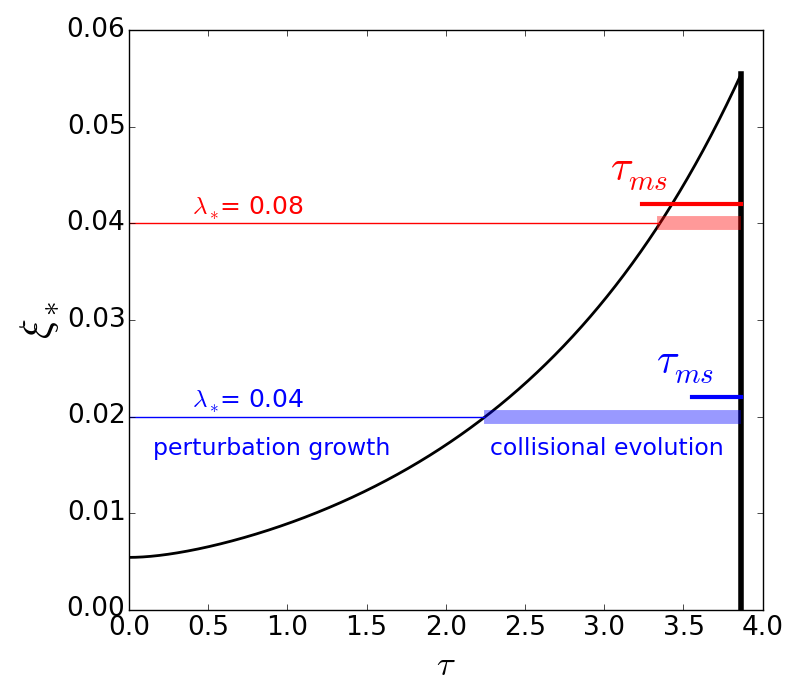
\includegraphics[width=\textwidth]{Figures/1_tau_ms.png}
        \caption{Regimes of overdensity evolution}
        \label{Fig:1_tau_ms}
    \end{subfigure}
    \begin{subfigure}[b]{0.49\textwidth}
    	\centering
    	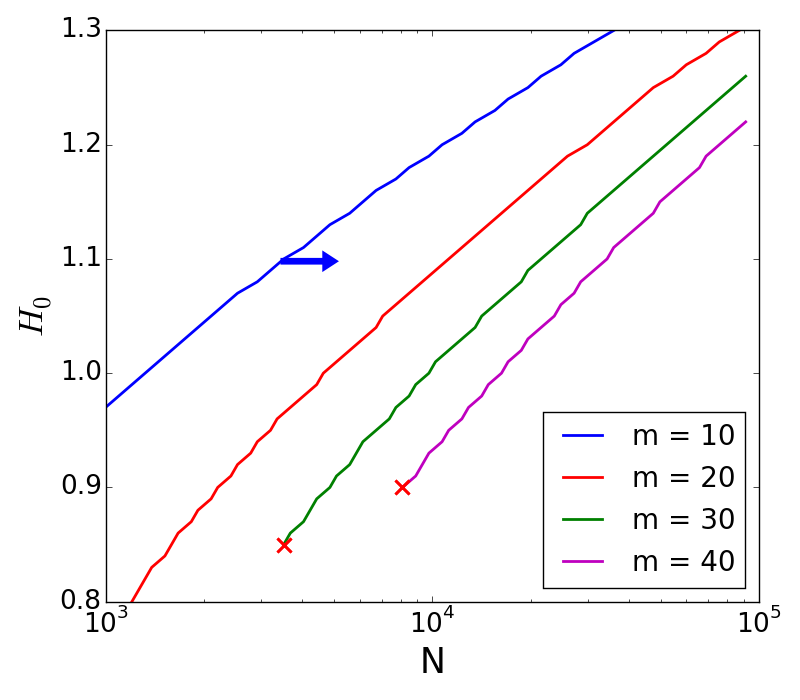
\includegraphics[width=\textwidth]{Figures/1_segregation_zone.png}
        \caption{Segregation domains}
        \label{Fig:1_segregation_zone}
    \end{subfigure}
\caption{(a): growth of perturbation $\xi_*$ over dimensionless time $\tau$ until the end of expansion at $\tau = 3.84$. An overdensity seeded with a wavelength $\lambda_*$ begins its collisional evolution when $\xi_*$ reaches $\frac{\lambda_*}{2}$. These regimes are illustrated for $\lambda_* =0.04$ and  $\lambda_* =0.08$. The overdensities have to evolve collisionally for at least $\tau_{ms}$ to mass-segregate. This time-scale is also shown for each case. The blue case evolve collisionally for several $\tau_{ms}$ and will end up mass-segregated, while the red case visibly don't have have time to segregate. Modes of large wavelength tend to produce less mass-segregated clumps. (b) for a given number of nodes $m$, a model on the right of the corresponding line (arrow for $m=10$) will have mass-segregated overdensities at the end of the expansion, will on the left, the collisional evolution is too short for segregation to sets in. The red crosses show the minimum N below which the modes cannot be resolved.} 
\label{Fig:0_perturbation_growth}
\end{figure}


We now make use of all previous development to follow the evolution of a perturbation in a given system and assess its dynamical state.

To ease comparisons with N-body calculations cast in standard H\'enon units, we set ${\cal M} = G = R_o = 1 $ and use $\Hub_0 = 1.0833 .. \simeq 1$ so that the total binding energy $E = -1/4$. The Hubble expansion proceeds until a time $t = \tau / \Hub_0 \simeq 3.87 / \Hub_0$, when $H = 0$ and the bounding radius $R$ reaches $R = a(\tau)R_o \simeq 2.4 R_o$. The evolution time up to that point coincides almost exactly with the {\it current} global system free-fall time of $\approx 4.1$ time units. System-wide collapse to the barycentre will ensue on the same time-scale, but now this process will involve the merging / scattering of several high-density clumps. 

The mass of individual stars follow a  truncated \cite{Salpeter1955} distribution function, where the distribution function $ dN/dm \propto m_\star^{-\alpha}$ with index $\alpha = 2.35$ for masses in the range  $0.3 M_\odot < m_\star < 100 M_\odot$ giving a mean value of $\simeq 1 M_\odot$. We chose this form mainly for simplicity, and for ease of calculations. 


Let us fix $\Estar = 6/7$, with $\Hub_0 = 1$ and set $N = 15 000$ as reference\footnote{The more accurate value is $\Hub_0 = 1 + 1/12 = 1.0833$ but we rounded up to 1 to simplify the discussion}. We compute a mean initial amplitude of perturbation $\xistaro \approx 0.005 $ with a shortest-resolved wavelength $\lambda_\ast \approx 0.04$. Fig.~\ref{Fig:1_tau_ms} displays the solution from integrating Eqs.~(\ref{Eq:1_system}). The amplitude $\xistar(\tau)$ grows monotonically and crosses the values $\lambda_\ast/2$ at $\tau \approx 2.3$~: thereafter the perturbation enters a non-linear regime of evolution during which the internal dynamics may become collisional $( \Delta\tau > \delta\tau_{ms})$. A second case is depicted on Fig.~\ref{Fig:1_tau_ms}, where the wavelength $\lambda_\ast = 0.08$ and the perturbation reaches amplitude $\xistar = \lambda_\ast/2$ at $\tau \approx 3.6$: there is then too little time left before the end of the Hubble expansion phase for a clump of stars to evolve collisionally ($\Delta\tau < \delta\tau_{ms}$). 





The dynamical state of individual clumps is clearly a question of membership $N_\lambda$ and mass spectrum as shown in (\ref{Eqn:Taums}). We have been arguing that most small-size clumps will show collisional internal evolution~: a small cluster of stars would lose low-mass stars in the process and so have an increased ratio of average-    to maximum stellar mass. It is not clear, then, whether this trend is strong enough to compensate for the (almost) linear dependence on membership. 
%Anticipating the results of the next section, we take $N_\lambda$ from Eq.~(\ref{Eqn:Clumpn}) to compute  a product  $N_\lambda / \ln 0.4 N_\lambda \times \langle m_\ast\rangle / \max(m_\ast) \sim 14 $ for the case of a Salpeter mass function truncated at $20 M_\odot$ ;  and about $3$ for a truncation value of $100 M_\odot$. In practice, the results of N-body 
%calculations yielded values scattered in the range [3, 14] $M_\odot$, 
%consistent with there being {\it no trend}  with clump membership $N_\lambda$. To inspect further the actual properties of clumps, we next turn to  N-body calculations. 






\section{N-body simulations}

After the previous analytical study, we present here the characteristics of actual, numerically obtained, Hubble-Lema\^itre fragmented models. The integration was performed with NBODY6, which treats the gravitational forces of stars with no softening of the potential. An example of the evolution of the system is shown on Fig~\ref{Fig:1_fragmentation}. 



\begin{figure}
\begin{center}
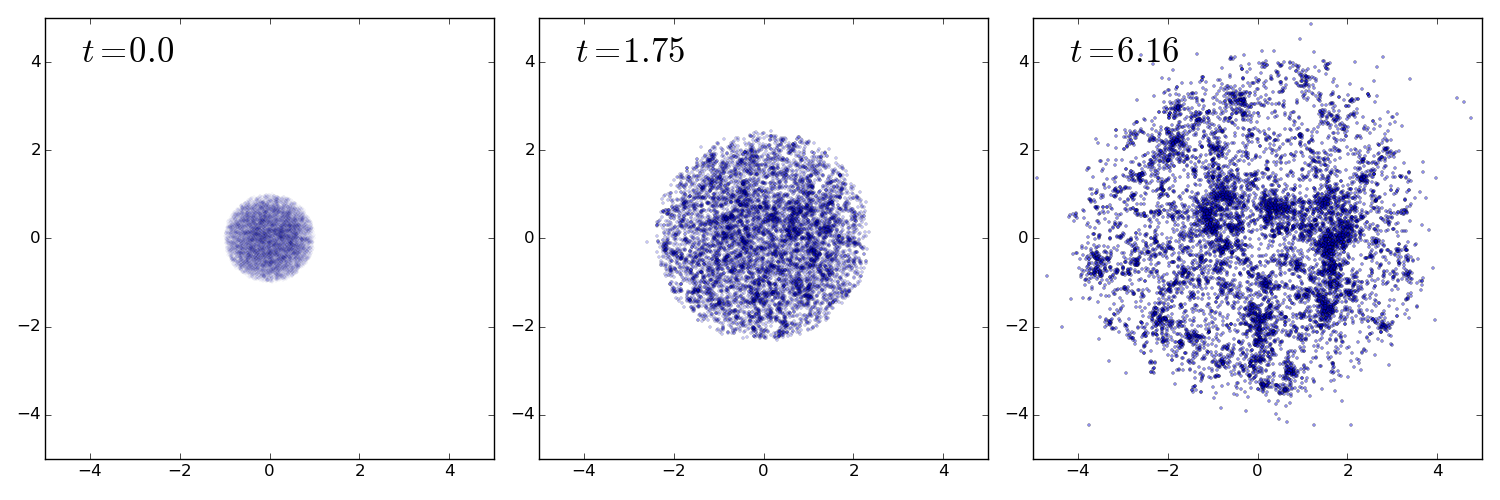
\includegraphics[width=\textwidth]{Figures/1_fragmentation}
\caption{Progressive fragmentation through the Hubble expansion. The left panel shows the initial uniform sphere; the middle panel, an intermediate step, slightly fragmented with a slowed down expansion; the right panel is the final stage, when the expansion has stopped and the fragmentation is fully developed. N=10000 particles were used in this N-body model, with $\Hub_0 = 1.0$. Time and coordinates are in H\'enon units.}
\label{Fig:1_fragmentation}
\end{center}
\end{figure}

%\subsection{Presentation of the runs}
%
%We draw $N$ stars from an Salpeter distribution function which we truncate by default to $100 M_\odot$~; in some calculations we will  use a lower bound of $20 M_\odot$, and in others we use identical masses. The code preserves the total energy and angular momentum to better than one part in $10^4$ for integration over $\sim 100 $ time units. The numerical integration starts with the expansion phase, but we will refer to the time at which this initial expansion stops ($H = 0$) as $t=0$, as we consider this dynamical state as initial conditions for cluster evolution. Memberships of 15000,40000 and 80000 were used, and 30 instances of each 15k model was performed to obtain statistically robust results.
%Table \ref{Tab:1_fragmentationmodels} summarises the main simulations used in this section to investigate the fragmentation of such systems.
%
%\begin{table}
%\begin{center}
%\caption{Summary of fragmentation models and their characteristics. These simulations started from an uniform sphere and were stopped when the expansion halted, at t=3 H.u . The third column shows the number of independent computations for each model.}
%\label{Tab:1_fragmentationmodels}
%\begin{tabularx}{\columnwidth}{XXlXX}
%\hline
%Name & N & Sampling & Mass range  \\
%\hline
%Rmh20 & 15000 & 30 & [0.35- 20 ]\\
%Rmh100 & 15000 & 30 & [0.3 - 100]\\
%Rmh1 & 15000 & 30 & 1.0 \\
%R40h20 & 40000 & 1 & [0.35- 20 ] \\
%R40h100 & 40000 & 1 & [0.3 - 100] \\
%R80h100 & 80000 & 1 & [0.3 - 100] \\
%\hline
%\end{tabularx}
%\end{center}
%\end{table}



\subsection{Clump finding algorithm}

As seen on Fig~\ref{Fig:1_fragmentation}, once expansion stops, the distribution is roughly spherical and visibly clumpy. By clump we mean here a local overdensity of stars. To characterize the model, is to characterize these substructures. Such analysis requires to find and isolate clumps, using an efficient clump-identification algorithm (or, {\it halo-finding} in cosmology).  Several methods are commonly used such as the HOP algorithm \citep{Eisenstein1998,Skory2010} which relies on attributing local densities to each particle and separating the clumps through density thresholds. The HOP algorithm is very robust on large cosmological data sets. However, our calculations have comparatively coarse statistics and noisy density fields. This issue, coupled with the  large number of free parameters of the HOP algorithm, makes the method less appealing. 

Instead we follow \cite{Maschberger2010} who adapted the minimum spanning tree (MST~; see e.g.\citealt{Allison2009b,Olczak2011}) technique to the detection of clumps. A spanning tree is a set of edges connecting a group of  particles but without closed loops~; the MST seeks to minimise the total length of the edges. One may then construct the MST for the whole system, and then delete all edges larger than a chosen cutting length, $d_{cut}$. The sub-sets that are still connected  are labeled as clumps. This process is illustrated in Fig \ref{Fig:1_MST}. In practice a minimum sub-set size $N_d$  is also chosen so as to avoid many small-N subgroups~: experience led us to choose  $N_d = 12$ for the minimum number of stars per clump. 

\begin{figure}
\begin{center}
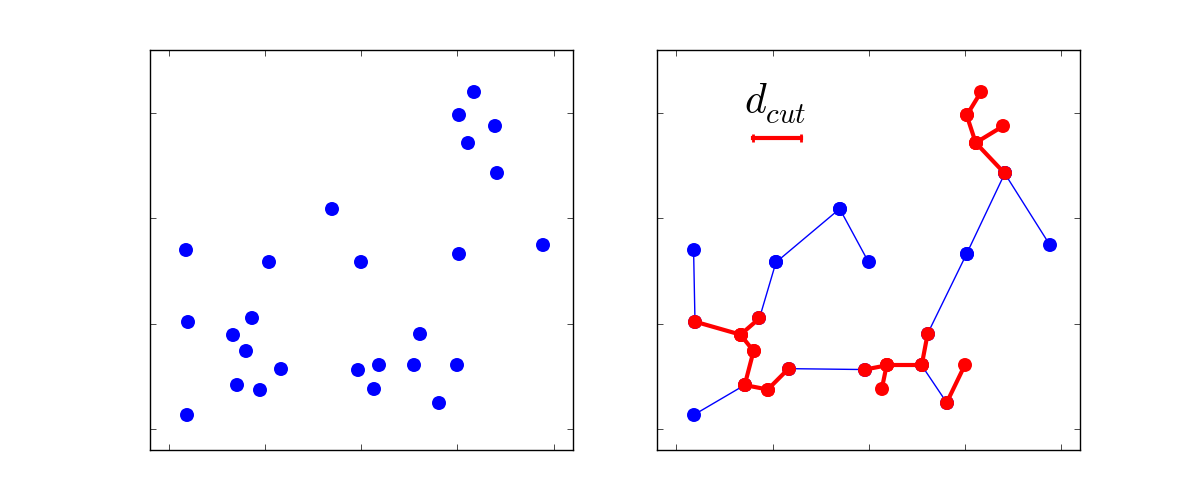
\includegraphics[width=0.8\columnwidth]{Figures/1_MST.png}
\end{center}
\caption{Illustration of a Minimum Spanning Tree and its use to isolate subgroups, using a cutting length $d_{cut}$.}
\label{Fig:1_MST}
\end{figure}


With $N_d$ fixed, the length $d_{cut}$ is then the only free parameter left. There is some freedom 
in choosing an appropriate value.
 
\cite{Maschberger2010} fixed the value of  $d_{cut}$ by visual inspection of clumps.
 We instead  identified  clumps in a fragmented system for a range of values for $d_{cut}$ and settled for the value  which optimised the number of identifications. This is shown on Fig.~\ref{Fig:1_Ndcut} for an N = 80k fully-fragmented Hubble model. For small $d_{cut}$'s, the number of detected clumps at first  increases rapidly. The rise is due  to the length $d_{cut}$ initially being small compared with the typical volume spawned by $N_d$ or more  nearest-neighbours. Beyond a certain value, a transition to another regime occurs, whereby the algorithm starts to connect previously separated clumps, counting them as one. The number of clumps thereafter begins to decrease. The value $d_{cut} \approx 0.025$ H.u optimises the outcome of the clump-search. This is a generic feature of the MST algorithm and we have adopted the same strategy throughout, adapting the value of $d_{cut}$ to the number $N$ of stars used. 

Another method to find the critical cutting length was used by \cite{Gutermuth2009,Kirk2011}. In these works, the authors build the MST, then trace the cumulative distribution function of all edges in the tree. In a clumpy configuration, there are at least two regimes: the "intra-clump" regime, with the majority of small edges, and the "inter-clump" regime with longer, scarcer edges. The intersection of a fit to these regimes provide a good cutting length for clump detection. This procedure was applied to our system and gave the same result than the clump counting, as shown on Fig~\ref{1_dcutcumulated}.

 

 
 \begin{figure}
\center
    \centering
    \begin{subfigure}[b]{0.49\textwidth}
    	\centering
    	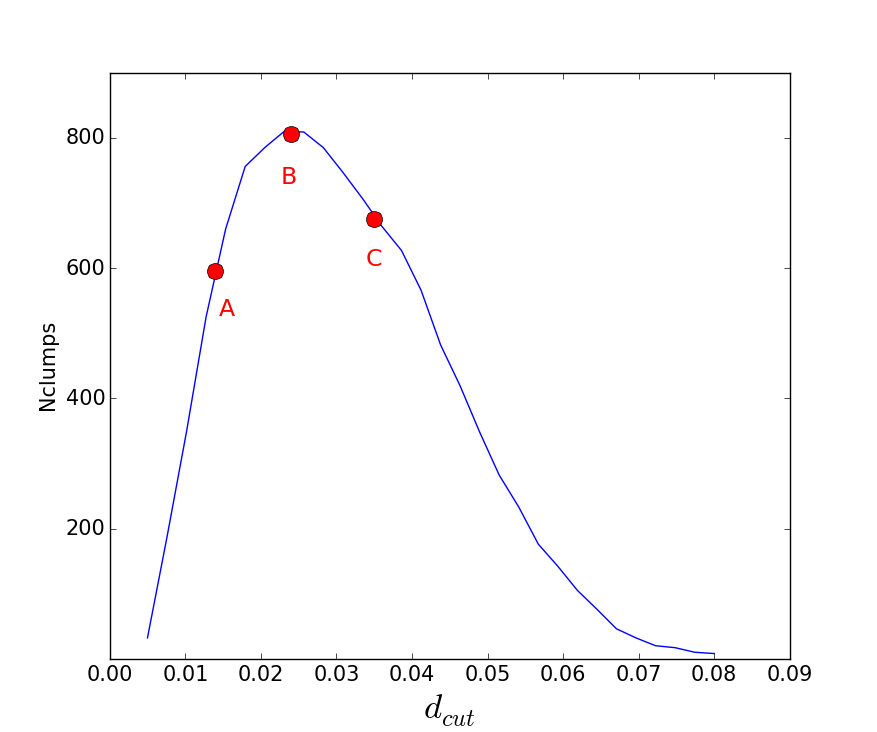
\includegraphics[width=\textwidth]{Figures/1_Ndcut.png}
        \caption{Number of clumps vs $d_{cut}$}
        \label{Fig:1_Ndcut}
    \end{subfigure}
    \begin{subfigure}[b]{0.49\textwidth}
    	\centering
    	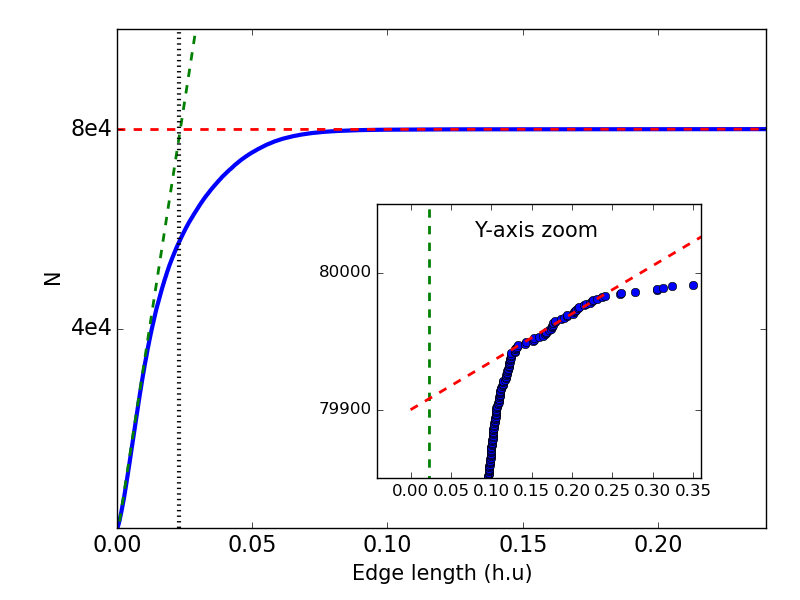
\includegraphics[width=\textwidth]{Figures/1_dcutdistribution.png}
        \caption{Cumulative distribution of MST edges}
        \label{Fig:1_dcutcumulated}
    \end{subfigure}
\caption{Two different methods to identify the critical $d_{cut}$ for clump detection. Both methods give the same value. For this 80k model, the value is 0.024 in H\'enon units. The ref linear fit on (b) was made on the linear portion with sufficient data points, discarding the very few further points departing from the tendency.}
\label{Fig:0_dcutchoice}
\end{figure}

 
   On Fig.~\ref{Fig:1_clumpsABC}, a sub-set of the model is shown where we have identified stars that belong to clumps with filled symbols. The three panels on that figure are each for a different value of $d_{cut}$, increasing from top to bottom. For the smallest value $d_{cut}$=0.015 H.u, clumps look somewhat truncated as we are still in the under-sampling regime and only their cores registered as clumps. The second, optimal, value $d_{cut}$=0.025 H.u produces visually well-isolated clumps. Finally, the third and  largest value is so that clumps begin to merge together~: this is shown by the unique clump identified in the bottom panel (filled blue squares).
   


\begin{figure}
\begin{center}
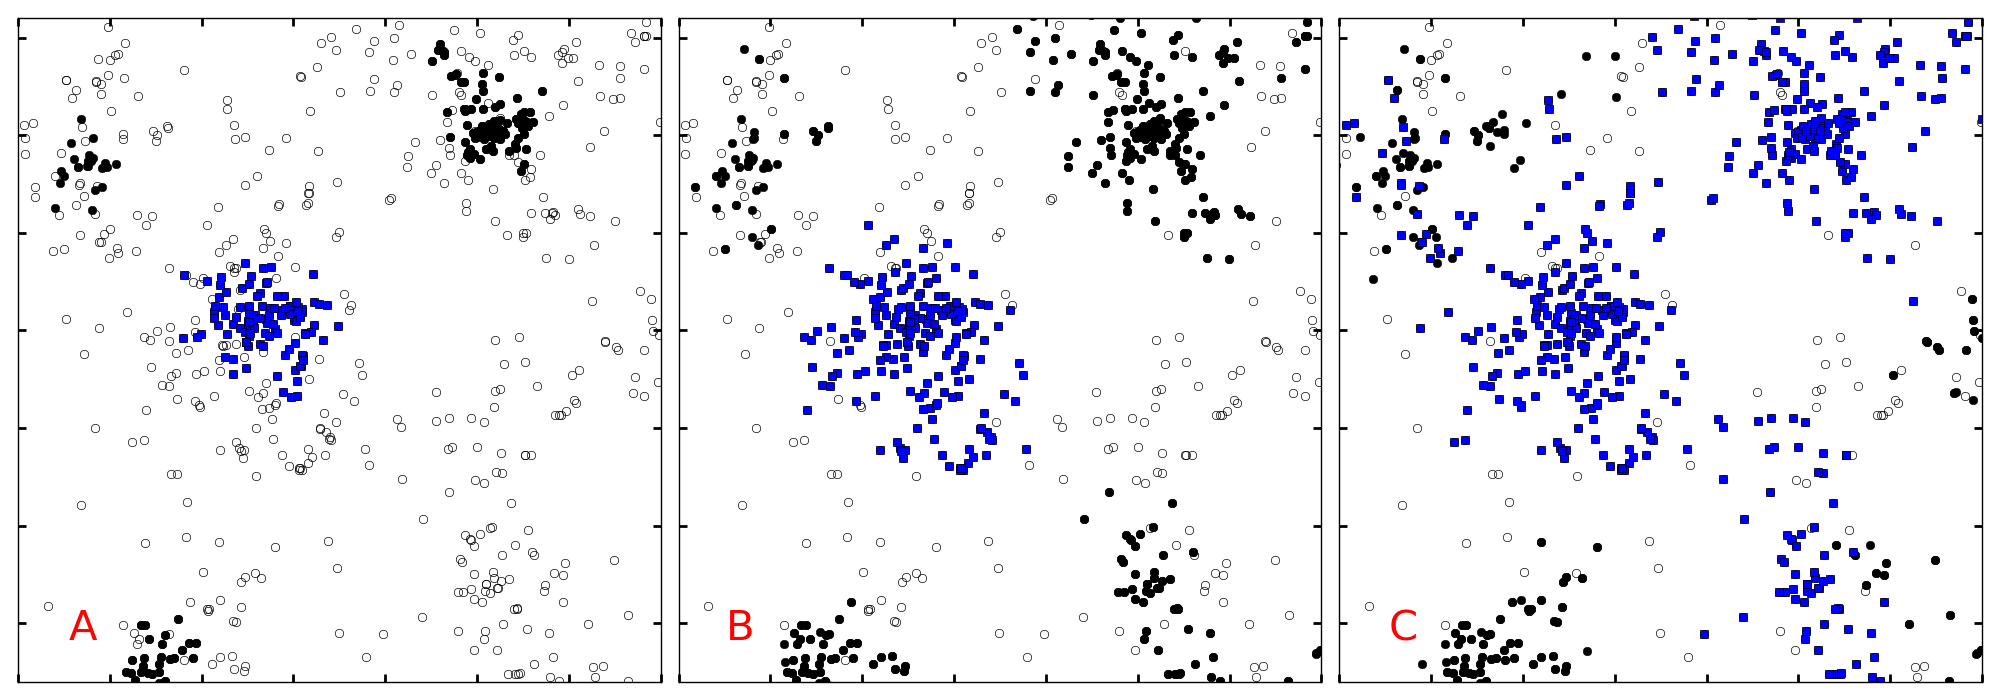
\includegraphics[width=0.9\columnwidth]{Figures/1_clumpsABC.png}
\end{center}
\caption{}
\label{Fig:1_clumpsABC}
\end{figure} 








%    %%%%%%%%%%%%%%%%%%%%%%%%%%%%%%%%%%%%%%%%%%%%
% Chapitre 2
%%%%%%%%%%%%%%%%%%%%%%%%%%%%%%%%%%%%%%%%%%%%


\chapter{La diffusion pour la médecine}
\label{Chapter2}

%    
%      % partie 2
%    \part{Méthodes de comparaison de deux populations de tenseurs de diffusion}
%    \label{Part2}
%    %%%%%%%%%%%%%%%%%%%%%%%%%%%%%%%%%%%%%%%%%%%%
% Chapitre 3 - INTRO
%%%%%%%%%%%%%%%%%%%%%%%%%%%%%%%%%%%%%%%%%%%%

\chapter*{Introduction}
\markboth{\textbf{Introduction}}{}
%---------------------------------------------------------------------------------------

%    %%%%%%%%%%%%%%%%%%%%%%%%%%%%%%%%%%%%%%%%%%%%
% Chapitre 3
%%%%%%%%%%%%%%%%%%%%%%%%%%%%%%%%%%%%%%%%%%%%

\chapter{Comparaison de groupes}
\label{Chapter3}

La comparaison de groupes consiste à chercher les changements, statistiquement significatifs, entre deux populations d'observations. 
En imagerie médicale, cela revient dans la plupart des cas d'étude, à comparer une population de sujets atteints d'une pathologie avec une population de sujets sains afin de mettre en avant les zones affectées par la maladie.
Cette méthode mathématique comporte deux parties centrales de traitements : la régression et l'analyse statistique. 
La première permet d'expliquer les observations grâce à des variables explicatives connues et associées à chaque observation, ainsi qu'à des régresseurs à estimer pour chacun des deux groupes.
La deuxième partie sert à tester si ces régresseurs présentent une différence statistiquement significative.
Ces parties sont généralement précédées par des pré-traitements tels que la correction des artefacts d'acquisition, le recalage et le fitrage.\\

% \minitoc

%----------------------------------------------------------------------------------------

\section{Contexte}
La comparaison de groupes s'inscrit dans un contexte de recherche pure. 
Il n'y a aucune application directe du praticien à son patient en clinique.
Par contre, les aboutissements d'une telle méthode apportent au médecin, une meilleure compréhension du mécanisme de la pathologie et une aide au diagnostique et au pronostique.
Les utilisateurs de cette approche sont aussi bien des scientifiques travaillant à résoudre les différents problèmes rencontrés (voir Section \ref{problematiques}) que des médecins analysant les résultats obtenus par des logiciels tels SPM ou SnPM\footnote{\url{http://warwick.ac.uk/snpm}}.

D'un point de vue parenté, cette méthode s'apparente à la comparaison longitudinale de deux images de tenseur consécutives d'un même patient \cite{Grigis2012}.
Le fait de prendre deux populations de sujets plutôt que seulement deux images longitudinales permet de réduire la variabilité inter-individus. 
Comme conséquence, cette approche rend le système statistique plus puissant pour détecter les zones de changements entre les deux groupes et non plus les variations structurelles d'un individu à un autre.

De plus, il est à noter que les cohortes ont des tailles de plus en plus importantes.
Comme exemples de base de données aux échelles nationale et internationale, Baltazar\footnote{\url{https://clinicaltrials.gov/ct2/show/study/NCT01315639?term=baltazar&rank=1}}, ADNI\footnote{\url{http://adni.loni.usc.edu/}} ou encore OSEP\footnote{\url{http://www.ofsep.org/fr/}} peuvent être citées.
La grande taille des échantillons dans un modèle statistique est un atout car cela rend les résultats obtenus plus fiables.


\section{Problématiques}
\label{problematiques}
Dans cette section, les différents problèmes intrinsèques à la comparaison de groupes seront abordés.
Trois axes principaux ont été dégagés et sont exposés dans l'ordre suivant : 
les problématiques liées à la multivariabilité des données, les problématiques provenant de la pré-étape de recalage et
les problématiques dûes à la géométrie du tenseur de diffusion.
Les travaux de cette thèse ont consisté à apporter des réponses ou encore à évaluer l'influence de ces trois points.

\subsubsection*{Problématique liée à la dimension des données}
Ce paragraphe n'est pas un état de l'art. 
Il sert simplement à introduire aux lecteurs les problèmes rencontrés à cause de la dimension des données.
Un état de l'art détaillé est proposé dans la prochaine section (voir \secref{etat_art}).\\
La multi-dimensionnalité des données est le problème majeur des images du tenseur de diffusion autant pour les pré-traitements que pour les traitements. 
Les tenseurs s'expriment sous forme de matrice de dimension 3, symétrique et définie positive, $D \in Sym^{+}(3)$~\cite{Basser1994} :
\begin{center}
    $\textbf{D} = \left[\begin{array}{ccc}
    D_{11} & D_{12} & D_{13}\\
    * & D_{22} & D_{23}\\
    * & * & D_{33}
    \end{array}\right]$
\end{center}
Toutes les informations permettant de décrire globalement la diffusion en un voxel, sont contenus dans cette matrice : 
diffusion radiale et axiale, orientation de la diffusion, diffusion moyenne ou encore fraction d'anisotropie.
Comme expliqué en début de chapitre, la comparaison de groupes consiste en deux opérations mathématiques : la régression et l'analyse statistique.
Elles peuvent être sous-divisées en opérations simples telles que l'addition, la soustraction, la division, la somme, la puissance ...
Ces opérations s'appliquent très facilement sur des scalaires.
Cependant appliquer une de ces opérations sur les images de tenseur de diffusion, revient à faire du calcul matriciel ce qui peut considérablement compliquer la tâche.
De plus, les hypothèses statistiques nécessaires pour la régression et l'analyse statistique peuvent totaltement différer entre le scalaire et la matrice.\\
Plusieurs techniques sont possibles pour traiter ce type de données. 
La première, la plus utilisée, consiste à extraire des scalaires (FA ou MD) de la matrice et à appliquer les méthodes de détection directement sur ces scalaires.
Deuxièment, des méthodes proposent de s'occuper seulement des 6 éléments supérieurs de la matrice en les concatenant dans un vecteur.
\begin{center}
    $vect(\textbf{D}) = \left[\begin{array}{cccccc}
    D_{11} & D_{12} & D_{13} & D_{22} & D_{23} & D_{33}
    \end{array}\right]^{T}$
\end{center}
Troisièment, certaines techniques s'appliquent directement sur la matrice entière du tenseur de diffusion.
%%%%%%%%%%%%%%%%%%%%%%%%%%%%%%%%%%%%%%%%%%%%%%%%%%%%%%%%%%%%%%%%%%%%%%%%%%%%%%%%
\subsubsection*{Problématique liée à la géométrie de l'espace des tenseurs}
Comme expliqué au \chapref{Chapter1}, page \pageref{Chapter1} du manuscrit, un tenseur de diffusion $\textbf{D}$ 
est représenté mathématiquement par une matrice de dimension 3, symétrique et définie positive, $\textbf{D} \in Sym^{+}(3)$~\cite{Basser1994}.
La définition positive du tenseur se vérifie si toutes ses valeurs propres sont strictement positives.
Cette géométrie particulière implique que l'espace du tenseur n'est pas un espace Euclidien mais un cône convexe défini dans cet espace vectoriel. 
Dans ce sous-espace, des métriques de l'espace Euclidien restent stables mais elles n'imposent aucune contrainte sur la positivité des tenseurs.
Certaines opérations entrainent des valeurs propres nulles ou négatives.
Prenons comme exemple simple, le résultat de la différence Euclidienne de deux tenseurs $\textbf{D}_{diff}$. 
Dans tous les cas, la matrice résultat est symétrique $\textbf{D}_{diff} \in Sym(3)$ mais pas forcément définie positive.

Dans ce contexte, plusieurs travaux ont été consacrés au développement de métriques, précédemment définie sur l'espace Euclidien, 
appliqués à un espace non plus \og plat \fg mais \og courbé \fg pour lequel les valeurs propres nulles ou négatives se situent à l'infini. 
Il est question de l'espace Riemannien, souvent représenté par une shpère.
La distance est alors définie, de manière intrinsèque, comme un chemin géodésique entre deux points.
Dans ces précédents travaux~\cite{Pennec1999,Pennec2004,Pennec2006}, Pennec a appliqué les métriques appartenant à des variétés Riemanniennes aux tenseurs de diffusion
permettant de préserver leur nature positive.

\begin{figure}[htpb]
    \centering
    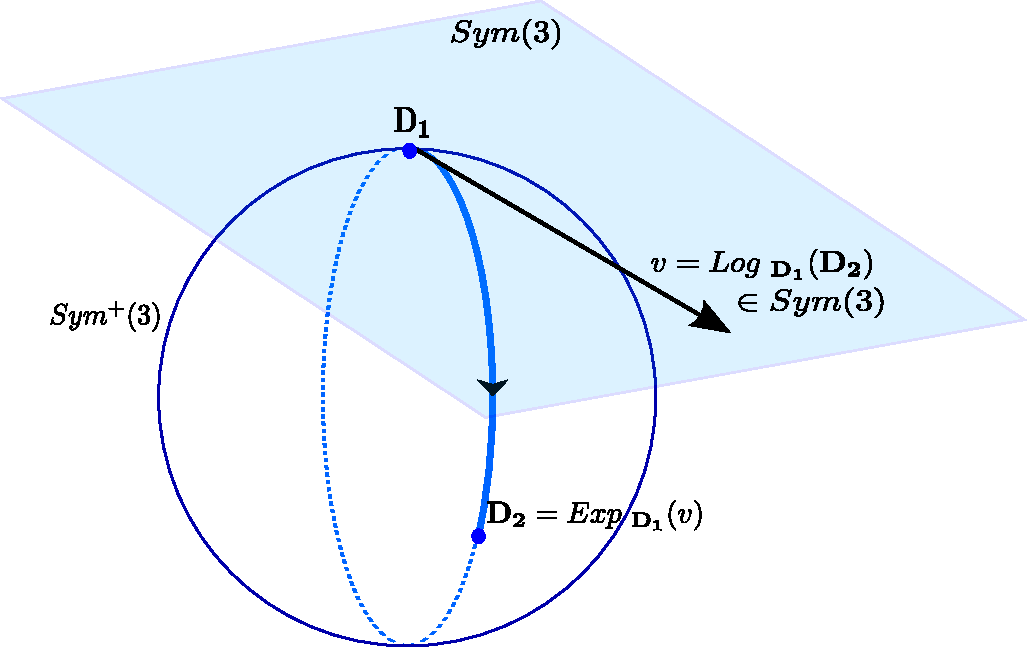
\includegraphics[scale=0.6]{Images/log_exp_map_sphere.pdf}
    \caption{\label{fig_log_exp_map} Illustration des cartes Riemanniennes logarithmique et exponentielle.}
\end{figure}

Cependant, à cause de la courbure de l'espace, l'implémentation de ces méthodes devient plus complexe et le temps d'exécution des calculs est considérablement plus long.
Dans l'optique d'éviter ces contraintes tout en conservant les propriétés théoriques convenables de l'espace Riemannien, 
de nouvelles métriques, appelées Log-Euclidiennes, sont proposées par~\cite{Arsigny2005,Arsigny2006} dans un cadre Riemanien.
Elles permettent de faire des \og aller-retours \fg entre un tenseur $\textbf{D}_\textbf{2}$ appartenant à l'espace des matrices symétriques définies positives $Sym^{+}(3)$ 
et son log-tenseur associé $Log_{\ \textbf{D}_\textbf{1}}(\textbf{D}_\textbf{2})$ de l'espace des matrices symétriques $Sym(3)$,
via le plan tangentiel au tenseur $\textbf{D}_\textbf{1}$ (voir le graphique en \figref{fig_log_exp_map}).
Par conséquent, l'enchainement suivant est rapide d'exécution, simple à implémenter et il garantit que le résultat est bien un tenseur de diffusion.
Le tenseur $\textbf{D}_\textbf{2}$ est projeté sur l'espace vectoriel associé au tenseur $\textbf{D}_\textbf{1}$.
Ensuite les métriques Euclidennes sont appliquées sur le log-tenseur $Log_{\ \textbf{D}_\textbf{1}}(\textbf{D}_\textbf{2})$ et $\textbf{D}_\textbf{1}$.
Enfin, le résultat peut être projeté de nouveau dans l'espace courbé.

Des travaux ont déjà évalué l'impact de telles métriques pour divers problèmes de traitements sur les tenseurs~\cite{Arsigny2006,Pasternak2010},
mais aucun ne précise la plus appropriée à utiliser, particulièrement dans le contexte de la comparaison de groupes.
%%%%%%%%%%%%%%%%%%%%%%%%%%%%%%%%%%%%%%%%%%%%%%%%%%%%%%%%%%%%%%%%%%%%%%%%%%%%%%%%%%%%%
\subsubsection{Problématique liée à l'étape du recalage}
C'est une étape fondamentale des pré-traitements en imagerie médicale. 
La comparaison de groupes nécessite une mise en correspondance spatiale des structures anatomiques afin de présenter les résultats en terme de regions neuro-anatomiques.
Cette étape permet de placer toutes les images des deux populations dans un même espace commun.

Nous pouvons décrire de manière très succincte le processus d'une telle étape.
Une étape de recalage consiste en une estimation du champ de déformations suivie par une application de ce champ aux images et d'une interpolation.
Plusieurs éléments composent la partie estimation de cette technique : des primitives à mettre en correspondance, un critère de similarité $f$, une transformation $t \in T$ ( $T$ étant le domaine des transformations), une méthode d'optimisation et bien évidemment deux images (une image source $I_s$ et une image de référence $I_r$). 

\begin{equation}
    \min_{t \in T} f(I_r, t(I_s) )
    \label{eq_recalage}
\end{equation}

Pour chaque élément de cette liste, il y a des sous-catégories : transformations globales ou locales, critère de similarité mono-modal ou multi-modal, type de primitives utilisées (voxels, surface, centre de gravité ...) ou encore le type de géométrie des transformations (rigide, affine et non-linéaire).
Dans la littérature, de nombreux travaux proposent des états de l'art complets sur l'étude du recalage en imagerie 
médicale~\cite{Noblet_PhD,Klein2009,Sotiras2013,Oliviera2014} dont certains sont plus spécifiques aux image du tenseur de diffusion~\cite{Zhang2007,Wang2011,Schwarz2014}.
Notre bibliographie s'est orientée autour de techniques de recalage sans structure particulière utilisant tous les voxels de nos images.
% image d'un pipeline 

Deux problématiques liées à l'étape du recalage appliqué aux images de tenseurs de diffusion se dégagent : l'interpolation et la ré-orientation des tenseurs.
En effet, dans le contexte du ITD, l'application d'un champ de transformations peut rencontrer de nombreuses difficultés, notamment dûes à la nature du tenseur de diffusion.\\

Premièrement, l'interpolation de deux tenseurs n'est pas évidente. 
Une interpolation linéaire de deux tenseurs avec une métrique Euclidienne de forme identique mais d'orientation perpendiculaire, 
un vertical et l'autre horizontal, produit une shpére et non pas un tenseur orienté à 45 degrés.
Ce problème rejoint celui présenté ci-dessus avec le paragraphe sur \og Problématique liée à la géométrie de l'espace des tenseurs \fg.
La \figref{fig_interpolation} illustre une interpolation linéaire des tenseurs avec trois métriques, une de chaque géométrie.\\
\begin{figure}[htpb]
    \centering
    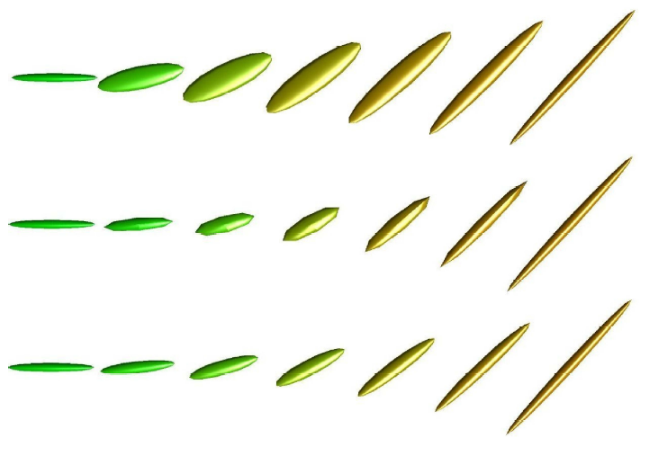
\includegraphics[scale=0.8]{Images/interpolation_arsigny.pdf}
    \caption{\label{fig_interpolation} Illustration~\cite{Arsigny2005} d'interpolation linéaire des tenseurs avec des métriques différentes. \textbf{Haut} : métriques Euclidenne, \textbf{Milieu} : métrique Riemannienne. \textbf{Bas} : métrique Log-Euclidienne}
\end{figure}

Deuxièment, l'orientation des tenseurs après l'application de la transformation estimée peut se révéler particulièrement contraignante.
Dans l'image source transformée, les voxels prennent, par tranformée inverse, les tenseurs présents dans l'image source avant recalage.
Ces tenseurs ont une décomposition spectrale qui permet d'obtenir les axes de l'ellipsoïde ($\overset{\rightarrow}{e_1}$, $\overset{\rightarrow}{e_2}$, $\overset{\rightarrow}{e_3}$) 
et les valeurs propres associées ($\lambda_1$, $\lambda_2$, $\lambda_3$).
Cette décompostion n'a pas pris en compte les tranformations subies par l'image.
Ainsi dans l'image source tranformée, les tenseurs auront les même décompositions spectrales et par conséquent, les même orientations.
Prenons comme exemple de tranformation, illustré par la \figref{fig_reorientation}, un simple rotation de 45 degrés.
L'image (a) représente l'image source de base.
L'image (b) montre l'image (a) ayant subie une rotation de 45 degrés. 
Il est visible que les tenseurs n'ont pas suivi la rotation et reste tels qu'ils sont dans l'image (a).\\

\begin{figure}[htpb]
    \centering
    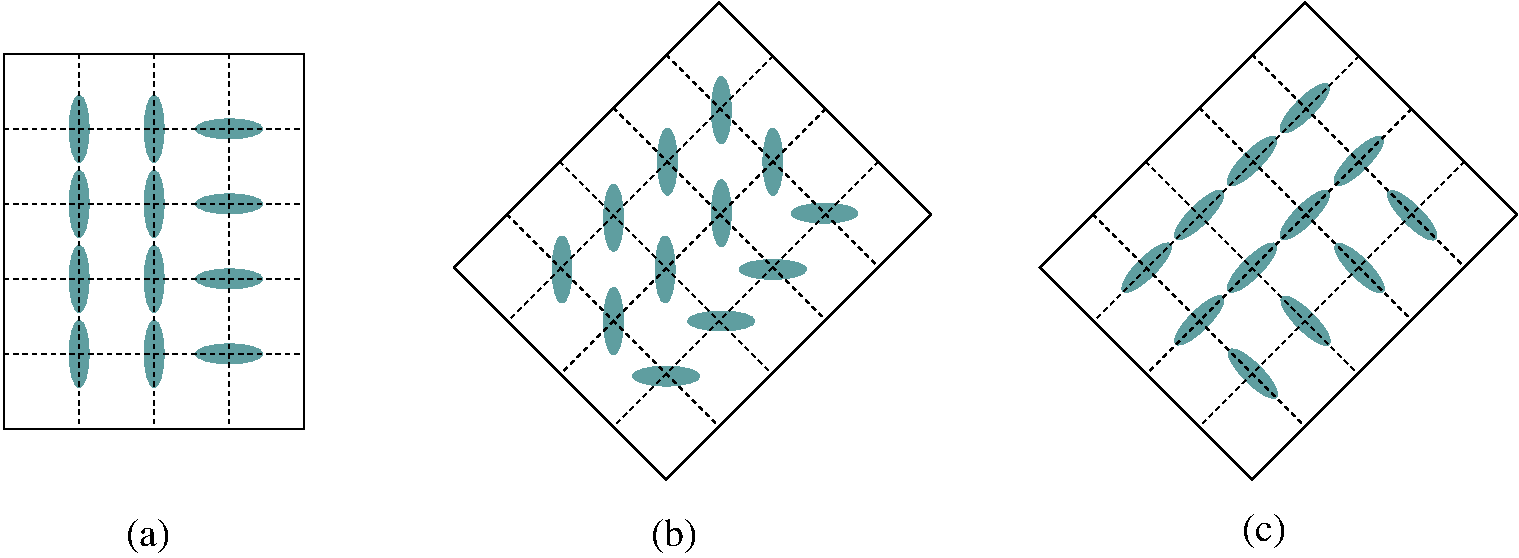
\includegraphics[scale=0.6]{Images/reorientation.pdf}
    \caption{\label{fig_reorientation} Illustration simple du problème de ré-orientation des tenseurs : rotation d'une image de tenseurs de diffusion de 45 degrés. (a) image d'origine, (b) image après application du champ de transformation,
    (c) image après application du champ de transformation et ré-orientation}
\end{figure}


\section{État de l'art en imagerie du tenseur de diffusion}
\label{etat_art}
En premier lieu, nous précisons que cet état de l'art ne s'intéresse qu'aux méthodes de détection de changements spécifiques
à l'imagerie du tenseur de diffusion et à la comparaison de groupes.
De nombreux articles et doctorats portent sur la détection de changements dans les divers autres domaines.
Pour une liste plus générale des références bibliographiques sur la détection de changements en imagerie de diffusion 
se réferrer au manuscrit de thèse d'Antoine Grigis \cite{Grigis_PhD}.\\

Les méthodes de détection peuvent être classées en trois grandes familles : 
les méthodes utilisant les indices scalaires dérivés du tenseur (FA ou MD), 
celles basées sur les vecteurs déduit du tenseur $vect(\mathbf{D})$
et enfin celles prenant en compte toute la matrice du tenseur $\mathbf{D}$.

La famille la plus grande est celle des méthodes basées sur les indices scalaires.
En effet, ces méthodes ne souffrent pas de problèmes de multi-dimensionnalité, ni de problèmes de variétés (voir \secref{problematiques}) : 
les indices scalaires commes leur nom l'indique sont des scalaires définis sur le domaine Euclidien.\\



Des modèles utilisant la matrice entière du tenseur ont aussi été développées \cite{Zhu2009, Schwartzman2010, Yuan2012, Bouchon2014, Kim2014} 
mais elles doivent faire face à l'incapacité du cadre euclidien pour tenir compte de la définie-positivité d'un tenseur de diffusion.\\

Comme expliqué dans la \secref{problematiques}, deux variétés avec des métriques prenant en compte la définie-positivité des tenseurs ont été proposées :
le Log-Euclidien \cite{Arsigny2006} et le domaine Riemanien \cite{Pennec1999}.\\

Quelques travaux ont déjà évalué l'impact des différentes métriques (Euclidiennes, Log-Euclidennes et Riemmaniennes) 
pour divers problèmes de traitement d'image \cite{Arsigny2006, Pasternak2010}, 
mais il n'y a toujours pas de consensus sur la variété la plus appropriée pour le traitement des tenseurs de diffusion, 
en particulier dans le contexte de comparaison de groupes.



\section{Pré-traitements}
\label{sec:preprocessing}
Cette section présente les trois pré-traitements implémentés dans la chaine de traitements : 
la correction des artefacts liés à l'acquisition,  l'estimation des tenseurs, le recalage qui permet de placer tous les sujets dans un même référentiel anatomique 
et enfin l'étape de filtrage permettant de lisser les observations afin de réduire le bruit et ainsi à améliorer les détections statistiques.

\subsection{Corrections des artefacts d'acquisition}
L'IRM de diffusion permet d'acquérir une série d'images pondérées en diffusion (DWI)
à partir de laquelle est estimée l'image du tenseur de diffusion (ITD).
Lors de l'acquisition, des artéfacts peuvent apparaître 
ce qui peut entraîner des distorsions importantes et compromettre les résultats des études.
Ils sont référencés dans la revue \cite{Jones2010}.
La plupart sont corrigés lors des pré-traitements afin d'obtenir des données 
les plus fiables possibles pour les analyses statistiques.
Pour cela, nous avons utilisé la méthode \og eddy\_current \fg de la librairie FSL\footnote{\url{http://fsl.fmrib.ox.ac.uk/fsl/}}.
% De plus, habituellement les gradients de diffusion sont normalisés mais nous avons eu un cas où ce n'était pas le cas. Nous avons alors dû corriger cette erreur et par défaut nous avons inclus une normalisation dans notre chaine de traitements. Cette opération par défaut est importante même si elle n'est que peu de fois exécutée car il suffit d'une série d'image avec des gradients de diffusion non normalisés pour fausser les résultats de la chaine de traitement.

\subsection{Estimation pondérée des tenseurs de diffusion}
La méthode classique d'estimation des tenseurs est celle des \og moindres carrés \fg.
Elle, ainsi que ses limites, sont décrites plus tôt dans le manuscrit (voir \chapref{Chapter1}).
Dans notre chaine de traitements, nous avons opté pour une méthode pondérée des moindres carrées proposé par \cite{Zhu2007} car
elle tient compte du fait que le bruit est un mélange de plusieurs bruits distribués différemment.
Les $n$ mesures pondérées en diffusion pour chaque voxel s'exprime sous la forme d'un triplet $(S_i, r_i, b_i)$ pour $i=1\ldots n$.
L'équation du signal acquis, et par conséquent bruité, s'écrit de la manière suivante après une transformée logarithmique pour linéariser le signal exponentiel : 
\begin{center}
    $log(S_i) = log(S_0) - b_i\textbf{r}_\textbf{i}^T\textbf{D}\textbf{r}_\textbf{i} + \eta_i$
\end{center}
Avec $S_i$ la $i^\text{ème}$ image pondérées en diffusion, $S_0$ l'image sans pondération, $b_i$ la b-valeur correspondante,
$\textbf{r}_\textbf{i} = (r_{i,1}, r_{i,2}, r_{i,3})^T$ le $i^\text{ème}$ vecteur de gradient de diffusion, $\eta_i$ le bruit lié à l'aquisition 
et enfin $\textbf{D}$ le tenseur de diffusion.
La méthode impose aux gradients de diffusion d'être distribués sur la sphère unité. 
Cela requière une normalisation au préalable des $n$ directions des gradients de diffusion pour qu'ils remplissent la condition suivante :
$\textbf{r}_\textbf{i}^{T}\textbf{r}_\textbf{i} = 1$.
L'estimation est initialisée par une méthode des moindres carrés classique suivie par plusieurs itérations $k_0 = 1\ldots 5$ d'une estimation par les moindres carrés pondérés.
Cette méthode est efficace et rapide d'autant plus que, comme démontré dans l'article \cite{Zhu2007}, 
une seule itération suffit lorsque le nombre de gradients de diffusion est égal ou supérieur à 30.
L'algorithme est détaillé ci-dessous par \algoref{algo:estimation_tenseur_2}.

\begin{center}
    \begin{minipage}[c]{0.9\textwidth}
	\begin{algorithm}[H]
	    \vspace*{0.5em}
	    \Data{
		$log(S_i) = z_i^T\theta + exp(-z_i^T\theta)\sigma\epsilon_i$ avec
		$z_i^T = (1, -b_i(r_{i,1}^2, 2r_{i,1}r_{i,2}, 2r_{i,1}r_{i,3}, r_{i,2}^2, 2r_{i,2}r_{i,3}, r_{i,3}^2))$
		et $\theta = (log(S_0), D_{11}, D_{12}, D_{13}, D_{22}, D_{23}, D_{33})$}\vspace*{1em}		
	    \Res{Estimation des 7 paramètres de $\theta$ : $\theta^{(k_0)} = (log(S_0), D_{11}, D_{12}, D_{13}, D_{22}, D_{23}, D_{33})$}
	    \Deb{
		initialisation $k = 0$ : $\hat{\theta}^{(k)} = ( \sum_{i=1}^{n} z_i z_i^T )^{-1} \sum_{i=1}^{n} z_i\ log(S_i)$\;\vspace*{1em}
		\Pour{$k_0$ itérations}{
		    $w_i^{(k)} = exp(2z_i^T\hat{\theta}^{(k)})$\;\vspace*{1em}
		    $\hat{\theta}^{(k+1)} = (\sum_{i=1}^{n} w_i^{(k)}z_iz_i^T)^{(-1)} \sum_{i=1}^{n} w_i^{(k)}z_i\ log(S_i)$\;
		}
	    }\vspace*{0.5em}
	    \caption{\label{algo:estimation_tenseur_2}Estimation du tenseur de diffusion par les moindres carrés pondérés}
	\end{algorithm}
    \end{minipage}
\end{center}

Pour mesurer la différence entre les méthodes des moindres carrées classiques et des moindres carrées pondérées, 
nous avons simulé un jeu de données de diffusion (type DWI) de synthèse basé sur les simulations introduites par \cite{Zhu2007} dans la section 3.1 de son article.
Nous avons effectué les deux estimations pour différentes valeurs du rapport signal sur bruit.
Pour chaque méthode, nous avons calculé l'erreur quadratique moyenne entre l'image de tenseurs d'origine et l'image de tenseurs estimée.
Nous avons mesuré une réduction d'erreur de 9\% en utilisant cette méthode comparée avec un moindres carrés classique.\\
{\color{red}ILLUSTRATIONS}

\subsection{Recalage}
L'état de l'art sur le sujet du recalage est disponible dans la \secref{problematiques} présentant les problématiques \ref{problematiques} en page \pageref{problematiques}.
Dans ce paragraphe, les trois méthodes de recalage utilisées dans la thèse seront exposés, ainsi que les raisons qui nous ont poussés à ces choix en particulier. 
Au cours de la thèse, nous nous sommes intéressé à l'influence que le recalage peut avoir sur les résultats des méthodes de détection. 
Et notamment aux fausses détections que peuvent engendrer une mauvaise ré-orientation ou une mauvaise estimation des déformations.
Pour répondre à la problèmatique présentée, nous avons sélectionné deux type des recalage différents : 
un recalage basé sur les cartes de scalaire avec une ré-orientation des tenseurs après l'application du champ de déformations 
et un recalage basé sur les cartes de tenseurs avec une ré-orientation des tenseurs directement intégrée de manière analytique dans la fonction de coût.

\subsubsection*{Recalage sur les images de FA}
La première méthode~\cite{Noblet2006} appartient au type de techniques le plus utilisée par la communauté en comparaison de groupes pour le ITD : 
les recalages qui estiment les champs de déformations sur les cartes de fraction d'anisotropie (FA) dérivées des images de tenseurs.

Cette méthode fonctionne en deux étapes.
Dans un premier temps, elle va estimer les transformations par la méthode des moindres carrées en se basant sur l'information mutuelle des images de FA.
Puis, dans un deuxième temps, sachant qu'il reste de petites distorsions anatomiques entre les images, 
un second recalage plus raffiné est effectué à l'aide d'une méthode non-rigide 
qui va estimer un modèle de déformation paramétrique multi-échelles toujours basé sur l'information mutuelle.
Ce recalage déformable peut être très puissant et compenser toutes les différences, de type anatomique ou pathologique, entre les images.
Pour éviter cela,~\cite{Noblet2006} propose d'imposer une contrainte de préservation de la topologie ainsi qu'un terme de régularisation.

Une fois les transformations finales estimées, elles sont appliquées sur les images de tenseurs en utilisant la méthode de 
Préservation de la Direction Principale~\cite{Alexander2001} pour ré-orienter les tenseurs correctement.

\subsubsection*{Recalage sur les images de tenseurs}
La deuxième technique appartient à la nouvelle génération qui estime les transformations directement sur les images de tenseurs.
Le défi du recalage d'images de tenseurs de diffusion est la multi-dimension des données et leur ré-orientation lors de l'application des transformations.
Une analyse comparative complète sur les différences entre 6 recalages basés scalaire et 2 basés tenseurs sont présentés par~\cite{Wang2011}.
Dans leur étude, la méthode \dtitk~\cite{Zhang2006, Zhang2007, Keihaninejad2013} montre les meilleurs résultats d'après les trois critères d'évaluation qu'ils proposent.
Les auteurs concluent en recommandant l'algorithme \dtitk par rapport aux autres méthodes déformables basées sur les tenseurs.
Cet outils de recalage est disponible en ligne\footnote{\url{http://www.nitrc.org/projects/dtitk}}.\\

La méthode \dtitk permet d'estimer les 12 paramètres d'une transformation affine $\textbf{p}$.
Cette estimation est faite morceau par morceau ce qui rend le champ des transformations globales non-linéaire.
L'expression de la transformation affine $F$ est décomposée en 3 matrices de base appliquées au voxel $x$ : 
\begin{equation}
    F(x) = (QS)x + T
    \label{fct_affine_dtitk}
\end{equation}
avec $T$ une matrice de translation, $S$ une matrice de pure déformation et $Q$ une matrice de pure rotation.
L'application de cette matrice $Q$ permet de ré-orienter un tenseur $\textbf{D}$ : $Q\textbf{D}Q^t$~\cite{Alexander2001}.
La méthode définit une fonction de coût $O$ qui intègre de façon explicite cette ré-orientation des tenseurs dans son expression :
\begin{equation}
    O(\textbf{p}) = \int_{\mathcal{R}^3} \|\textbf{D}_s((QS)x + T) - Q\textbf{D}_rQ^t\|^2dx
    \label{fct_cout_dtitk}
\end{equation}
avec $\textbf{D}_r$ et $\textbf{D}_s$ respectivement le tenseur de référence et le tenseur source à déformer.\\

De plus, la méthode \dtitk estime les 12 paramètres $\textbf{p}$ de la transformation affine morceau par morceau sur des régions de taille égale $\Omega_i$
en imposant une contrainte de continuité inter-régions.
Pour cela, l'algorithme essaie de minimiser la différence entre les transformations affines de deux régions.
\begin{equation}
    \int_{\Omega_i\bigcap\Omega_j} \|F_i(x) - F_j(x)\|dx
    \label{fct_cont_dtitk}
\end{equation}
L'expression analytique des équations \eqref{fct_cout_dtitk},\eqref{fct_cont_dtitk} permet une résolution du problème par les gradients conjugués.\\

\begin{figure}[htpb]
    \centering
    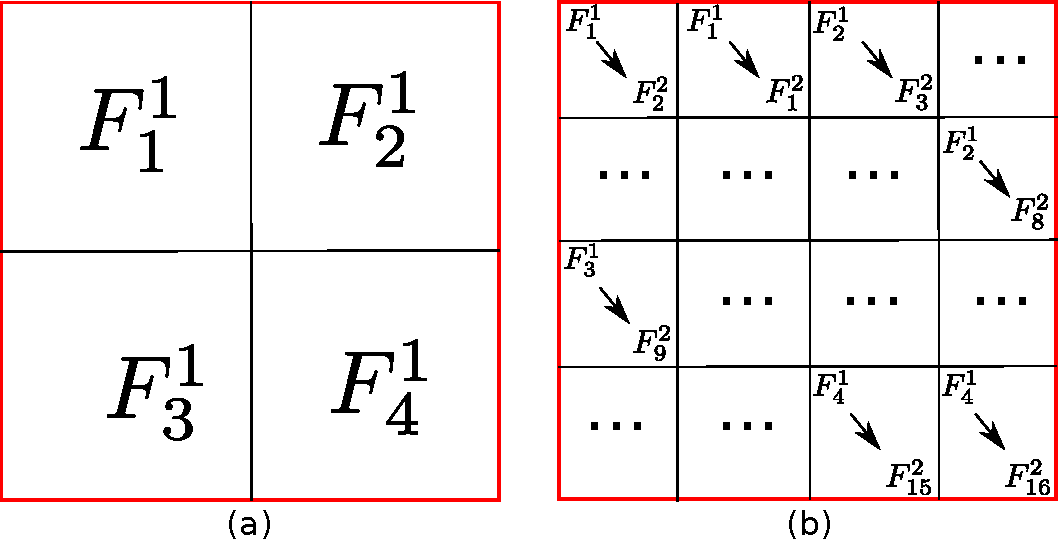
\includegraphics[scale=0.7]{Images/dtitk_hierarchie.pdf}
    \caption{\label{fig_dtitk_hierarchie}Illustration de l'approche hiérarchique de l'algorithme \dtitk.
    (a) est la représentation du partage initial ($n=2$) grossier de l'image avec les estimations des transformations sur chaque région.
    (b) est la représentation au niveau supérieur ($n=4$) avec l'estimation des transformations initialisée par les transformations du niveau inférieur.}
\end{figure}
Les transformations finales sont estimées par une approche hiérarchique illustrée par la \figref{fig_dtitk_hierarchie}.
L'algorithme estime les premières transformations $F_i^{n}$ sur une image découpée grossièrement ($n=4$ régions sur chaque côté de l'image 3D).
Par la suite, il raffine son estimation en partageant plus finement l'image ($n=8, 16$) et en initialisant les transformations avec celles du niveau inférieures.

\subsubsection*{Recalage sur les images d'IRM de T1}
Dans son article, \cite{Tustison2014} met en avant un fait important :
estimer les tranformations du recalage sur les même cartes de données sur lesquelles l'analyse statistique
sera effectuée, revient à introduire un biais dans le modèle favorisant les détections.
Il appelle ce phénomène, \og circularity bias \fg et cela se traduit pas une augmentation générale des p-valeurs.
Pour supprimer ce biais, \cite{Tustison2014} conseille d'éviter les recalage basés sur le même jeu de données 
que celui utilisé pour l'analyse statistique lors de la compraison de groupes.
À la place, un recalage en deux étapes est recommandé. 
Dans un premier temps, un recalage multi-modal et intra-individu est effectué entre les cartes de FA vers les cartes d'IRM de T1.
Il est suivi, dans un deuxième temps, par un recalage sur les cartes T1 inter-individus combinant une méthode affine et une méthode non-linéaire~\cite{Noblet2006}.


\subsection{Filtrage}


Après l'étape de recalage, il est recommandé d'utiliser un filtre sur les images de tenseurs dans le but de lisser les observations, de réduire le bruit présent et ainsi contribuer à améliorer les détections statistiques.

%    %%%%%%%%%%%%%%%%%%%%%%%%%%%%%%%%%%%%%%%%%%%%
% Chapitre 4
%%%%%%%%%%%%%%%%%%%%%%%%%%%%%%%%%%%%%%%%%%%%

\chapter{Méthode linéaire}
\label{Chapter4}

Ce chapitre présente les méthodes de détection développées au cours de la thèse.
De manière classique, la comparaison de groupes en ITD s'effectue sur les cartes scalaires dérivées des images de tenseus, 
comme les cartes de \fa (FA) ou de \md (DM) via le logiciel SPM\footnote{\url{http://www.fil.ion.ucl.ac.uk/spm/}}.
Cependant, chaque indice scalaire caractérise une seule et unique information sur la diffusion.
Ainsi, les autres informations sur la diffusion ne sont pas prises en compte dans le modèle scalaire.
Par contre, les six éléments du tenseur englobent toute l'information de la diffusion.
C'est dans l'optique d'éviter cette perte d'information que nous avons proposés de nouvelles méthodes 
qui sont des extensions de la méthode classique aux images du tenseurs de diffusion.
Elles sont basées sur le \mlg (MLG) et consistent en une régression multi-linéaire suivi d'un test statistique.
Le MGL consiste à représenter les données comme des combinaisons linéaires de variables explicatives et de valeurs d'intérêt, nommés régresseurs à  estimer.
À partir de ces régresseurs, un test statistique nous permet de savoir si ils sont statistiquement différents.
Dans ce chapitre, les notations mathématiques seront les suivantes : $a$ est une variable, $\{a_i\}_{i=1..N}$ est un ensemble de $N$ variables, 
$\mathbf{a}$ est une matrice ou un vecteur, $\hat{a}$ est l'estimée de la variable.
De plus, les régressions multi-linéaires présentées utilisent les métriques du domaine Euclidien.
Le chapitre suivant étudie l'impact des différentes métriques (Euclidiennes, Log-Euclidiennes et Riemanniennes) sur la comparaison de groupes.\\

% \minitoc

%----------------------------------------------------------------------------------------

\section{Régression multi-linéaire}
Cette première section est une introduction au formalisme mathématique de la régression multi-linéaire.
L'expression de \mlg est présentée ainsi que l'étape d'estimation des régresseurs par la méthode des moindres carrés.
Mathématiquement, le concept de régression multi-linéaire peut être décrit de la manière suivante :\\
\begin{adjustwidth}{1cm}{}
    Soit $\mathbb{M}$ une variété et $\{y_i\}_{i \in [1..N]} \in \mathbb{M}$ les observations de $N$ individus pouvant être caractérisés 
    par $K$ variables explicatives (ou covariables) $\{x_{i,j}\}_{j \in [1..K]} \in \mathbb{R}$ telles que l'âge, le genre ou l'affiliation aux différents groupes.
    La régression consiste à estimer une fonction $f : \mathbb{R}^{K} \mapsto \mathbb{M}$ 
    qui fait correspondre au mieux les différents couples $(\{x_{i,1} \dots x_{i,K} \} ,y_i)$
    en minimisant les résidus $\varepsilon_i = y_i - f(\{x_{i,1} \dots x_{i,K} \})$. 
    Pour cela, le modèle utilise des métriques définis sur la variété $\mathbb{M}$.\\
\end{adjustwidth}

Notons que la variété $\mathbb{M}$ peut être : le domaine Euclidien ($\mathbb{M} \subset \mathbb{R}$), le domaine Log-Euclidien ($\mathbb{M} \subset \mbox{Sym}(3)$) 
ou encore le domaine Riemannien ($\mathbb{M} \subset \mbox{Sym}^+(3)$).
Dans cette section, les observations appartiennent à la variété Euclidenne $\mathbb{M} \subset \mathbb{R}$.
Une étude sur l'impact du choix de la variété des métriques sur les résultats de la comparaison de groupes est présentée au \chapref{Chapter5}.

\subsection{Expression du \mlg : $\mathbb{M} \subset \mathbb{R}$}
Le \mlg est un outil fondamental dans les analyses statistiques d'observations.
Il permet d'expliquer les observations avec des variables explicatives en les mettant sous forme de système linéaire
à résoudre $\mathbf{y} = \mathbf{Ax}$.
Deux cas de figures différents sont possibles : le premier cas où les observations sont des scalaires, alors la régression est dite univariée, 
et le second cas qui correspond à une régression multivariée, c'est-à-dire que les observations sont des vecteurs.
Les deux cas d'observations sont présentés dans les paragraphes suivants.
Malgrès cette différence dans les modèles, ils font tous les deux l'hypothèse forte que les résidus $\varepsilon_i$ sont identiquement distribués 
et indépendants $\varepsilon_{i} \overset{idd}{\sim} \mathcal{N}(0, \sigma^2)$ avec $\sigma^2$ la variance du bruit additif du modèle.
De plus, la méthode d'estimation des variables d'intérêt est la même et sera présentée dans la sous-section suivante.

\subsubsection*{Cas d'observations univariées}
Dans la cas d'observations univariées, le \mlg (MLG) permet de représenter une observation $y_{i=1..N} \in \mathbb{R}$, 
comme une combinaison linéaire des variables explicatives $\{x_{i,j}\}_{j \in [1..K]} \in \mathbb{R}$ 
et des variables d'intérêt, les régresseurs $\{\beta_j\}_{j \in [1..K]}$:
\begin{alignat}{2}
    f &:\ \mathbb{R}^{K} &&\mapsto \mathbb{R} \nonumber \\
    &{}\left[\begin{array}{c}
x_{1}\\
\vdots\\
x_{K}
\end{array}\right] &&\mapsto y_i = \beta_{1}x_{i,1} + \beta_{2}x_{i,2} + \dots + \beta_{K}x_{i,K} + \varepsilon
\label{glm}
\end{alignat}
Les différents paramètres à estimer de l'équation \eqref{glm} sont les coéfficients des régresseurs $\{\hat{\beta}\}$.
Chaque régresseur est associé avec une variable explicative et représente l'effet de cette covariable sur l'observation.
Un exemple classique de covariable pour les maladies dégénératives du système nerveux central chez l'homme est celui de l'âge. 
Lorsque un groupe de sujets sains est comparé avec un groupe de sujets atteints d'une pathologie neurodégénérative, 
l'atrophie cérébrale dûe à l'âge des individus peut apparaîre comme régions pathologiques, or elles ne sont pas nécessairement représentatives de la maladie étudiée.
Pour éviter cela, la variable de l'âge est incluse dans le système et permet au modèle d'expliquer une partie de l'observation par cette covariable.

L'estimation du résidu du modèle, représenté par la variable $\varepsilon$, 
découle de celle des régresseurs $\hat{\varepsilon} = y - \hat{\beta_{1}}x_{i,1} + \dots + \hat{\beta_{K}}x_{i,K} $.
Si les variables explicatives ont une distribution centrée alors il faut imposer $x_{1} = 1$ 
(dans la suite du manuscrit, nous considèrerons que nous sommes dans cette configuration).
Un exemple simple de régression multi-linéaire sur un cas univarié
est illustré par la \figref{regression_2D} dans le cas 2D ($K=2$).
Sur la figure, les points bleus correspondent aux couples $(\{1, x_{i,2}\},y_i)$ et la droite affine rouge représente la fonction $f(\{1, x_{i,2}\})$.\\
\begin{figure}[ht]
    \centering
    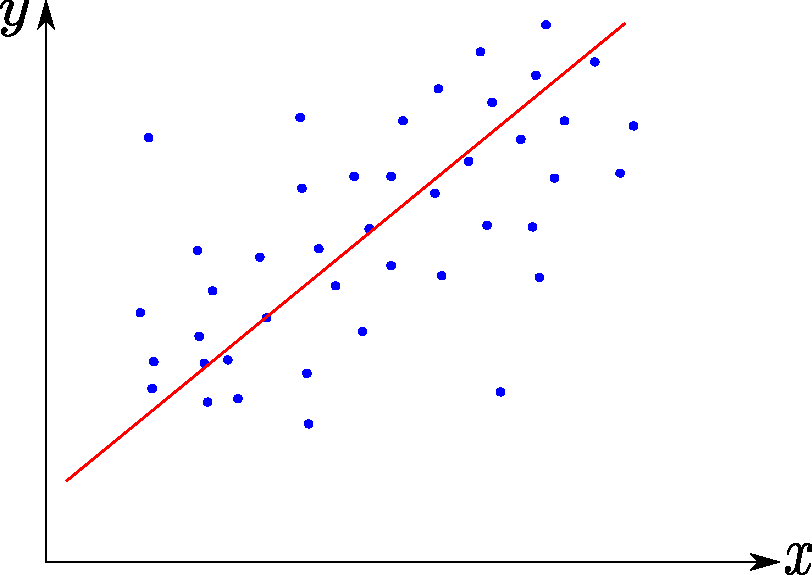
\includegraphics[scale=0.5]{Images/regression_2d.pdf}
    \caption{\label{regression_2D} Illustration d'une régression multi-linéaire 2D ($K=2$). 
    Les points bleus correspondent aux couples $(\{1, x_{i,2}\} ,y_i)$ et la droite affine rouge à la fonction $f(\{1, x_{i,2}\})$.}
\end{figure}

Dans le cas multi-linéaire d'un modèle avec $N$ observations,
l'équation \eqref{glm} peut facilement s'écrire sous la forme matricielle.
Les observations sont stockés dans le vecteur $\mathbf{Y} = \left[y_1\dots y_i\dots y_N\right]^{t}$, 
les variables explicatives associées aux observations dans la matrice $\mathbf{X}\left[i,j\right] = x_{i,j} \mbox{ avec } \mathbf{X}\left[i,0\right] = 1$,
les régresseurs sont dans le vecteur $\mathbf{B} =\left[\hat{\beta_{1}}\dots \hat{\beta_j}\dots \hat{\beta_K}\right]^{t}$.
et les résidus dans le vecteur $\mathbf{e} = \left[\varepsilon_1\dots \varepsilon_i\dots \varepsilon_N\right]^{t}$. 
Avec ce modèle, les résidus suivent tous la même distribution $\mathbf{e} \overset{idd}{\sim} \mathcal{N}(0, \sigma^2)$.
\begin{equation}
    \underbrace{\mathbf{Y}}_{N\times 1} = 
	      \underbrace{\mathbf{X}}_{N\times K}\underbrace{\mathbf{B}}_{K\times 1} + \underbrace{\mathbf{e}}_{N\times 1}
    \label{glm_mat}
\end{equation}

\subsubsection*{Cas d'observations multivariées}
Dans le cas dit \og mutlivariées \fg, pour chaque individu, les observations sont des vecteurs $\{y_{i,m}\}_{m=1..M} \in \mathbb{R}$ 
et les variables explicatives $\{x_{i,j}\}$ sont les mêmes pour chaque élément du vecteur.
Ainsi l'équation \eqref{glm} peut être réécrite de la manière suivante :
\begin{alignat}{2}
    f &:\ \mathbb{R}^{K} &&\mapsto \mathbb{R}^{N}\times\ \mathbb{R}^{M} \nonumber \\
    &{}\left[\begin{array}{c}
x_1\\
\vdots\\
x_K
\end{array}\right] &&\mapsto \left[\begin{array}{c}
\mathbf{y_1} = \left[y_{1,1} \dots y_{1,m} \dots y_{1,M} \right]\\
\vdots\\
\mathbf{y_N} = \left[y_{N,1} \dots y_{N,m} \dots y_{N,M} \right]
\end{array}\right]
\label{glm_multi}
\end{alignat}

Pour chaque élément des vecteurs, le \mlg décompose les données comme une combinaison linéaire des variables explicatives associées à l'individu
et des régresseurs associés à l'élément du vecteur :

\begin{align}
    y_{1,m} &= \beta_{1,m}x_{1,1} + \beta_{2,m}x_{1,2} + \dots + \beta_{K,m}x_{1,K} + \varepsilon_{1,m} \nonumber\\
    y_{i,m} &= \beta_{1,m}x_{i,1} + \beta_{2,m}x_{i,2} + \dots + \beta_{K,m}x_{i,K} + \varepsilon_{i,m} 
\end{align}

Ce système se traduit en écriture matricielle pour le $m^\text{ème}$ élément du vecteur d'observation par l'équation \eqref{glm_mat_multi}. 
Ce modèle est équivalent à $M$ modèles univariés indépendants, un pour chaque composante $m$ des vecteurs d'observation 
avec la même matrice de dessin $\mathbf{X}$ que pour le cas univarié.

\begin{equation}
     \underbrace{\mathbf{Y_m}}_{N\times 1} = 
	      \underbrace{\mathbf{X_{}}}_{N\times K}\underbrace{\mathbf{B_m}}_{K\times 1} + \underbrace{\mathbf{e_m}}_{N\times 1}
    \label{glm_mat_multi}
\end{equation}

Le modèle représentant les performances académiques d'étudiants est un exemple simple pour illustré le cas d'observations multivariées.
Prenons une étudiante $i$ avec ses moyennes pour les deux sessions de partiels semestriels $y_{i,1} \mbox{ et } y_{i,2}$.
Sachant le nombre d'heure qu'elle a passé à étudier par semaine $x_{i,2}$, son QI $x_{i,3}$ et son rang de l'année précédente $x_{i,4}$, 
le mlg permet d'écrire un système pour $K=4$ variables explicatives (avec $x_{i,1} = 1$):

\begin{equation}
    \mathbf{y_i} =
    \left[\begin{array}{c}y_{i,1}\\y_{i,2}\end{array}\right] = 
    \left[\begin{array}{c}\beta_{1,1} + \beta_{2,1}x_{i,2} + \beta_{3,1}x_{i,3} + \beta_{3,1}x_{i,3} + \varepsilon_{i,1}\\
			  \beta_{1,2} + \beta_{2,2}x_{i,2} + \beta_{3,2}x_{i,3} + \beta_{3,2}x_{i,3} + \varepsilon_{i,2}\end{array}\right] \nonumber
\end{equation}

Pour une promotion entière composée de $N$ étudiants, le \mlg permet de représenter deux systèmes ($M=2$) de régression multi-linéaire \eqref{ex_glm_multi}.
Avec ce modèle, les deux vecteurs de résidus suivent deux lois normales différentes $\mathbf{e_m} \overset{idd}{\sim} \mathcal{N}(0, \sigma^2_m)$.

\begin{align}
    \mathbf{Y_1} = \mathbf{X}\mathbf{B_1} + \mathbf{e_1} \nonumber \\
    \mathbf{Y_2} = \mathbf{X}\mathbf{B_2} + \mathbf{e_2} 
    \label{ex_glm_multi}
\end{align}


\subsection{Estimation des régresseurs : la méthode des moindres carrés}
Le \mlg met en place un système linéaire à résoudre $\mathbf{Y} = \mathbf{XB}+\mathbf{e}$. 
Il représente les observations comme une combinaison linéaire de variables explicatives 
et de variables d'intérêt avec un bruit additif gaussien $\varepsilon_{i} \overset{idd}{\sim} \mathcal{N}(0, \sigma^2) \label{res_iid}$.
Pour résoudre ce système, il faut estimer les $K$ variables d'intérêt  $\{\beta_{j}\}_{j=1..K}$.
Le meilleur estimateur au sens du maximum de vraisemblance pour des observations avec un bruit additif gaussien est l'estimateur par la méthode les moindres carrés.
La méthode proprose de minimiser l'erreur quadratique entre les observations et la combinaison linéaire pour estimer les régresseurs $\{\hat{\beta}_{j}\}_{j=1..K}$.
\begin{align}
    \mathbf{\hat{B}} &= \arg\min_{B \in \mathbb{R}^{k}}{\|\mathbf{Y} - \mathbf{X}\mathbf{B} \|^{2}} \nonumber\\
     &= (\mathbf{X}^{t}\mathbf{X})^{-1}\mathbf{X}^{t}\mathbf{Y}
    \label{ls_reg}
\end{align}

Les propriétés asymptotiques de l'estimateur par les moindres carrés sont connues 
et le fait que les résidus du modèle suivent une distribution normale implique 
que les régresseurs suivent une loi de gaussienne de moyenne $E(\mathbf{B}) = \mathbf{\hat{B}}$ et de variance $Cov(\mathbf{B}) = \mathbf{\hat{\varSigma}}$
\begin{equation}
    \mathbf{B} \sim \mathcal{N}(\mathbf{\hat{B}}, \mathbf{\hat{\varSigma}})
\end{equation}
L'expression analytique de l'estimée de $\mathbf{\hat{B}}$ est donnée par l'équation \eqref{ls_reg} et $\mathbf{\hat{\varSigma}}$ peut en être directement déduite :
\begin{align}
    \mathbf{\hat{\varSigma}} &= \hat{\sigma}^{2}(\mathbf{X}^{t}\mathbf{X})^{-1} \label{ls_reg_VAR}\\
    \text{avec } \hat{\sigma}^{2} &= \frac{1}{N-K}\|\mathbf{Y} - \mathbf{X}\mathbf{\hat{B}} \|^{2} \label{ls_reg_var}
\end{align}

Dans le cas d'observations multivariées, il faut faire une estimation par les moindres carrés pour chaque équation du système \eqref{ex_glm_multi}.

\subsection{Exemple d'application aux images de scalaires}
Ce paragraphe est un exemple d'application du \mlg avec des observations univariées.
Il correspond à la méthode classique employée par SPM pour faire une comparaison de groupes en ITD sur des images de scalaires dérivées des images de tenseurs de diffusion.

Soit $N$ le nombre d'individus total divisé en deux groupes avec respectivement $N_1$ sujets sains et $N_2$ sujets atteints d'une pathologies.
L'observation $y_i$ représente la valeur d'un voxel $p$ de l'image de scalaire (par exemple l'image de \fa FA) pour le $i\text{ème}$ individu.
L'ensemble des observations $\{y_i\}_{i=1..N}$ correspond aux valeurs du voxel $p$ de tous les $N$ individus.

\begin{equation}
    \underbrace{\mathbf{Y}_{}}_{N\times 1} = \left[\begin{array}{c}
                                             y_1\\
                                             \vdots\\
                                             y_N
                                         \end{array}\right]
  \xrightarrow{\text{correspond à}} 
  \underbrace{\mathbf{Y}_{}^p}_{N\times 1} = \left[\begin{array}{c}
                                             FA_1^p\\
                                             \vdots\\
                                             FA_N^p
                                         \end{array}\right]
\end{equation}

Soit $K=3$ variables explicatives associées au modèle :
$x_{1,\cdot}=1$ est la constante de \og centrage \fg, 
$x_{2,\cdot}= \{0,1\}$ la covariale d'affiliation au groupe ($0$ si l'individu appartient au groupe sain et $1$ s'il appartient au groupe atteint)
et $x_{3,\cdot}$ la variable de l'âge.
La matrice de dessin s'écrit donc de la manière suivante.

$$\underbrace{\mathbf{X}_{}}_{N\times K} = \left[\begin{array}{ccc} 
                                             centre & gp & \hat{a}ge\\
                                             1 & 0 & 36\\
                                             1 & 0 & 28\\
                                             \vdots & \vdots & \vdots\\
                                             1 & 1 & 25\\
                                             1 & 1 & 37\\
					      \end{array}\right] $$

Grâce à la $2^{\text{ième}}$ covariable (celle du groupe), le \mlg permet de quantifier l'effet du groupe sur les observations. 
Ainsi, pour un voxel $p$ donné, il est possible d'évaluer si il appartient statistiquement plus au groupe sain ou au groupe atteint.
Par exmple, si un axone (passant par le voxel $p$) est dymélinisé par la pathologie
alors la valeur de la FA en ce voxel sera moins élévée que celle du voxel sain sans démyélinisation.
Ce voxel aura alors une forte probabilité d'être représentatif de la maladie.
La covariable de l'âge permet de corriger les effets dûs au vieillissement naturel du cerveau dans le modèle.
Il est également possible de voir cet effet de l'âge sur le cerveau en analysant le régresseur associé.

Il est intéressant de voir qu'il est inutile de résoudre un seul système \eqref{glm_mat} par voxel.
Une concaténation de toutes les valeurs des $V$ voxels dans la matrice $\mathbf{Y}$ est possible.
Cela permet d'estimer les $K$ régresseurs de chaque voxel en une seule et unique opération de pseudo-inverse.
\begin{equation}
    \underbrace{\mathbf{Y}}_{N\times V} = 
	      \underbrace{\mathbf{X}}_{N\times K}\underbrace{\mathbf{B}}_{K\times V} + \underbrace{\mathbf{e}}_{N\times V}
    \label{ex_glm_mat}
\end{equation}



\section{Cadre statistique}
Le test statistique est la deuxième étape de la comparaison de groupes.
Il permet de quantifier les effets des régresseurs de manière statistique pour chaque voxel de l'image.
Un effet est dit significatif si il traduit un réel écart entre les deux groupes, et permet ainsi de conclure à l'existence d'une différence.
Pour cela, un test d'hypothèse est défini, permettant de formuler une règle de décision pour statuer si la différence est significative ou si elle ne l'est pas.
Cette prise de décision est basée sur la notion d'erreur associée à une probabilité donnée par le résultat du test statistique.

\subsection{Tests d'hypothèse}
Un test d'hypothèse est un test statistique qui permet d'associer une valeur à une prise de décision dans le but de quantifier la confiance en une hypothèse.
Deux hypothèses peuvent être formulées dans un cadre statistique :\\
\begin{itemize}
    \item l'hypothèse nulle $\mathcal{H}_{0}$ qui exprime une absence d'effet. 
    Cela se traduit par le fait que pour un régresseur donné, il n'y a aucune différence significative entre les deux groupes. 
    Les écarts observés sont dûs au bruit et à la variabilité inter-individus.
    Suivant les résultats du test statistique, l'hypothèse nulle $\mathcal{H}_{0}$ est acceptée ou rejetée.\\
    \item l'hypothèse de rejet $\mathcal{H}_{1}$ qui représente l'hypothèse alternative si $\mathcal{H}_{0}$ est rejetée.\\
\end{itemize}

Dans le contexte de comparaison de groupes en imagerie médicale pour un voxel, l'hypothèse nulle définit $\mathcal{H}_{0}$\textit{ : aucun changement significatif}
et l'hypothèse alternative $\mathcal{H}_{1}$\textit{ : changement détecté significatif}.

\subsection{Règle de décision}
Dans ce cadre statistique, il y a deux vérités et deux décisions possibles, ce qui conduit à quatre configurations différentes (voir \tabref{tab_test_hypo}).
Elles entrainent deux types d'erreur qui sont les erreurs de première $\alpha$ et de deuxième $\beta$ espèce (voir \figref{loi_norm}).\\
\begin{itemize}
    \item la vérité correspond à l'hypothèse nulle $\mathcal{H}_{0}$ et le test accepte cette hypothèse. 
    Cela mène à une bonne détection avec une probabilité de $1-\alpha$, ou encore la probabilité d'avoir un Vrai Négatif ($VNeg$).\\
    \item la vérité est l'hypothèse nulle $\mathcal{H}_{0}$ et le test rejette cette hypothèse.
    Cela correspond à détecter un Faux Positif ($FPos$) avec une probabilité de $\alpha$.\\
    \item la vérité est l'hypothèse $\mathcal{H}_{1}$ et le test accepte cette hypothèse.
    Cette configuration mène à une bonne décision par la détection d'un Vrai Positif ($VPos$) avec une probabilité de $1-\beta$.\\
    \item la vérité est l'hypothèse $\mathcal{H}_{1}$ et le test rejette cette hypothèse.
    Ce cas correspond à la probabilité $\beta$ d'avoir un Faux Négatif ($FNeg$).\\
\end{itemize}

\begin{table}[ht]
  \centering
  \begin{tabular}{|c|c|c|}
      \hline
      \diagbox{Décision}{Vérité} & $\mathcal{H}_{0}$ & $\mathcal{H}_{1}$ \tabularnewline
      \hline
      $\mathcal{H}_{0}$ & $1-\alpha\ (VNeg)$ & $\beta\ (FNeg)$ \tabularnewline
      $\mathcal{H}_{1}$ & $\alpha\ (FPos)$ & $1-\beta\ (VPos)$ \tabularnewline
      \hline
  \end{tabular}
  \caption{\label{tab_test_hypo}Choix possibles lors de la décision : probabilité d'accepter ou de rejeter l'hypothèse $\mathcal{H}_{0}$ 
	    exprimée par l'erreur de première espèce $\alpha$ et de deuxième espèce $\beta$.
	    Les probabilités sont associées aux types de détections {$VNeg$, $VPos$, $FPos$, $FNeg$} correspondant respectivement 
	    aux nombres de Vrais Négatifs, Vrais Positifs, Faux Postitifs et Faux Négatifs.} 
\end{table}
\begin{figure}[ht]
    \centering
    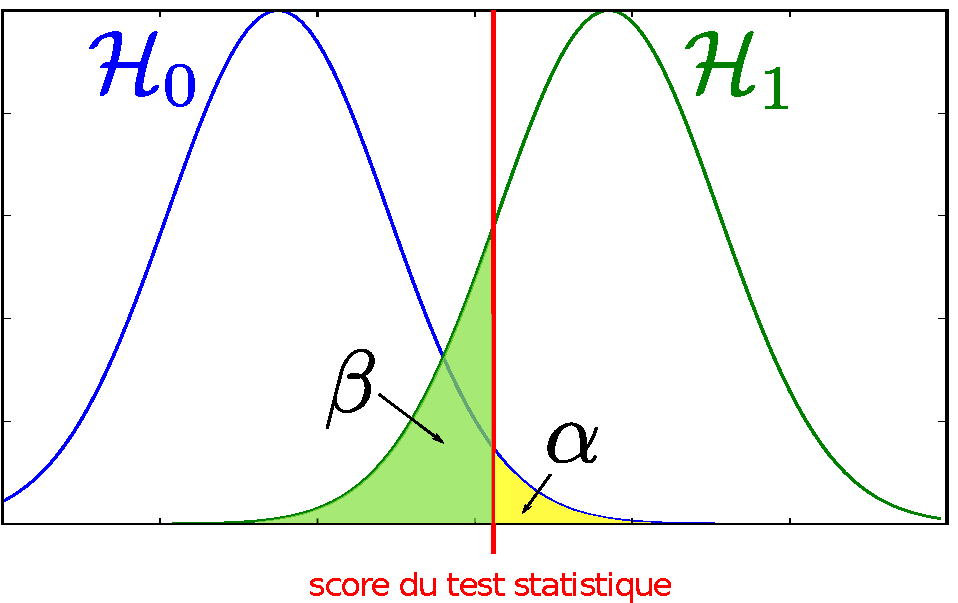
\includegraphics[scale=0.5]{Images/loi_norm.pdf}
    \caption{\label{loi_norm}Illustration des erreurs de première $\alpha$ et de deuxième $\beta$ espèce.}
\end{figure}

Il existe deux types de tests d'hypothèse : 
les tests paramétriques pour lesquels la loi de probabilité sous l'hypothèse $\mathcal{H}_{0}$ est connue ($f_0$)
et les tests non-paramétriques pour lesquels elle n'est pas connue.
En règle générale, la distribution sous l'hypothèse $\mathcal{H}_{1}$ n'est pas connue et ne peut pas être modèlisée.
Un état de l'art sur les différents tests paramétriques et non-paramétriques en détection de changements en imagerie de diffusion
est présenté dans le manuscrit de thèse \cite{Grigis_PhD}.\\

Dans le cas des tests paramétriques, il est possible de calculer une probabilité, nommée \textit{p-valeur} (voir \figref{calcul_p_valeur}), associée à une valeur statistique ($s$) du test.\\
\begin{equation}
    \text{\textit{p-valeur}} = \int_{seuil}^{\infty} f_0(s)ds
\end{equation}

\begin{figure}[ht]
    \centering
    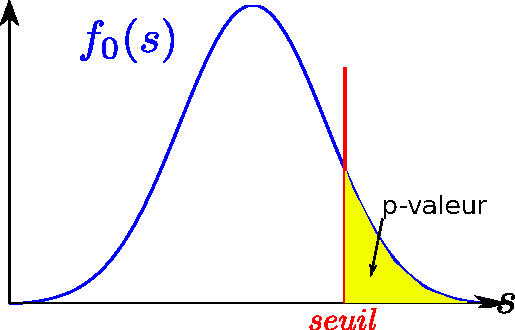
\includegraphics[scale=0.6]{Images/calcul_p_valeur.pdf}
    \caption{\label{calcul_p_valeur}Calcul de la p-valeur : 
    aire sous la courbe $f_0(s)$ représentant la distribution sous l'hypothèse $\mathcal{H}_{0}$ pour une valeur statistique du test ($seuil$).}
\end{figure}

À partir de l'erreur de première espèce $\alpha$ ou de la \textit{p-valeur}, deux façons de procéder sont possibles.
La première consiste à imposer la valeur de l'erreur $\alpha$ et à calculer la valeur statistique ($seuil$) associée en fonction de la loi $f_0$.
Ensuite, l'hypothèse est acceptée ou rejetée si le résultats du test est, respectivement, inférieur ou supérieur à ce $seuil$.
La deuxième stratégie commence d'abord à calculer la \textit{p-valeur} associée à la valeur statistique ($seuil$) en fonction de la loi $f_0$
pour après la comparer avec la valeur souhaitée de l'erreur $\alpha$.\\

Dans le cas des tests non-paramétriques, la loi de probabilité sous l'hypothèse $\mathcal{H}_{0}$ est inconnue, 
rendant impossible la modélisation de la distribution et le calcul de \textit{p-valeur}.
Il est néanmoins possible d'estimer la fonction $f_0$ en utilisant une méthode de permutation introduite par \cite{Chung2008}.
De manière générale, une permutation correspond à une interversion de deux valeurs de la matrice dessin $x_{i_{1},j}$ et $x_{i_{2},j}$,
$j$ étant à la variable d'intérêt (par exemple le groupe).\\
\begin{equation}
    \underbrace{
	  \left[\begin{array}{ccc} 
	  centre & gp & \hat{a}ge\\
	  1 & 0 & 36\\
	  1 & 0 & 28\\
	  \vdots & \vdots & \vdots\\
	  1 & 1 & 25\\
	  1 & 1 & 37\\
	  \end{array}\right]
      \ldots
	  \left[\begin{array}{ccc}
	  centre & gp & \hat{a}ge\\
	  1 & 1 & 36\\
	  1 & 0 & 28\\
	  \vdots & \vdots & \vdots\\
	  1 & 1 & 25\\
	  1 & 1 & 37\\
	  \end{array}\right]
      \ldots 
	  \left[\begin{array}{ccc}
	  centre & gp & \hat{a}ge\\
	  1 & 0 & 36\\
	  1 & 0 & 28\\
	  \vdots & \vdots & \vdots\\
	  1 & 0 & 25\\
	  1 & 1 & 37\\
	  \end{array}\right]
	  }_{T\ permutations} \nonumber
\end{equation}

La méthode de permutation consiste à calculer les scores du test non-paramétrique proposé pour $T$ permutations différentes.
L'histogramme de tous les scores obtenus permet d'estimer la loi de distribution sous $\mathcal{H}_{0}$.
À partir de cet histogramme et d'un niveau de significance $\alpha$ choisi, 
le calcule du score $seuil$ du test statistique (première stratégie présentée dans le paragraphe précédent) devient possible.
L'importance du nombre $T$ de permutations est évidente : pour $T=1000$ permutations, la plus petite \textit{p-valeur} est $0.001$. 
Pour avoir une plus grande précision, il faut donc augmenter le nombre de permutations.
Un inconvénient majeur à cette méthode est le temps de calcul qu'elle génére.
En comparaison, un test paramétrique effectue une opération alors que un test non-paramétrique va effectuer cette opération $T$ fois.

\subsection{Test statistique de comparaison utilisé}
Dans nos études, un test statistique de Fisher est utilisé pour évaluer si une des variables explicatives contribue de manière significative dans le modèle de régression.
Pour cela, le test compare, au sens des moindres carrés, les résidus de deux modèles imbriqués : 
un modèle dit \og complet \fg qui prend en compte toutes les variables explicatives ($\mbox{RSS}_{2}$)
et un modèle dit \og restreint \fg où la covariable d'intérêt est rejeté ($\mbox{RSS}_{1}$) :
\begin{equation}
    F = \frac{\displaystyle \frac{RSS_{1} - RSS_{2}}{\displaystyle p_{2} - p_{1}} }{\displaystyle \frac{RSS_{2}}{ \displaystyle N - p_{2}}}
    \label{test_stat}
\end{equation}
avec $ p_{2} \mbox { et } p_{1}$, représentant respectivement le nombre de variables explicatives des deux modèles et $N$ le nombre d'observations.
En supposant que les résidus suivent une distribution normale ($\varepsilon \sim \mathcal{N}(0, \sigma^2)$), 
$F$ suit une distribution de Fisher avec $p_{2}-p_{1}$ et $ N-p_{2} $ degrés de liberté,
sous l'hypothèse nulle $\mathcal{H}_{0}$ que le modèle 2 ne fournit pas un meilleur ajustement des variables explicatives aux données que le modèle 1.

L'hypothèse gaussianité des résidus est une hypothèse raisonnable dans un cadre Euclidien et Log-Euclidien mais elle n'est plus valable pour un cadre Riemannien.
Dans ce dernier cas, pour obtenir des cartes de \textit{p-valeur}, une méthode de permutation peut être utilisée mais cela demande des temps de calcul prohibitifs.


\section{Extension du \mlg aux tenseurs}
Dans la section précédente, nous avons montré un exemple d'application du \mlg aux images de Fraction d'Anisotropie.
Cette méthode fournit des résultats seulement sur des changements spécifiques à la FA.
Il manque, dans ce modèle, des informations sur la diffusion pour détecter tous les types de changements existants,
par exemple changements de diffusion moyenne ou encore modification d'orientation.
Ces informations multiples qui permettent de caractériser de manière générale la diffusion sont toutes contenues dans le tenseur de diffusion.
C'est dans cet optique de ne perdre aucnue information que nous avons développé une méthode basée sur le \mlg 
pouvant être appliquée sur des images de tenseur de diffusion.

Dans notre extension du \mlg aux tenseurs de diffusion, nous avons considéré trois stratégies : 
les deux premières sont basées sur des hypothèses d'homoscédasticité et d'hétéroscédasticité des données alors que
la dernière utilise l'information présente dans le voisinage du voxel analysé.
La première stratégie est un cas de \mlg avec des observations univariées alors que les deux autres utilisent des données mutlivariées.
Pour rappel, le tenseur $\mathbf{D}$ est un matrice symétrique définie positive de dimension 3.
Dans cette section, elle est exprimée comme un vecteur des six éléments supérieurs de la matrice :
$$vect\ (\mathbf{D})=\left[D_{xx}\ D_{xy}\ D_{xz}\ D_{yy}\ D_{yz}\ D_{zz}\right]^{t}$$

\subsection{Hypothèse d'homoscédasticité}
L'hypothèse d'homoscedasticité consiste à supposer que la variance du bruit de chaque élément du tenseur $D_{\largedot\largedot}^i$ est identique :
$\varepsilon_i \sim \mathcal{N}(0, \sigma^2)$.
Ce modèle se présente sous la même forme que le \mlg pour un cas d'observations univariées.
Pour prendre en compte toutes les informations liées à la diffusion, 
les six éléments du tenseur $\mathbf{D^i}$ du $i^\text{ème}$ sujet sont concaténés en un seul vecteur vertical 
$vec\ (\mathbf{D^i})=\left[D^i_{xx}\ D^i_{xy}\ D^i_{xz}\ D^i_{yy}\ D^i_{yz}\ D^i_{zz}\right]^{t}$  
et chaque élément du tenseur est considéré une observation.
Le modèle précédent passe donc de $N$ observations à un modèle composé de $N\times 6$ observations.

\begin{equation}
    \underbrace{\mathbf{Y}_{}}_{N\times 1} = \left[\begin{array}{c}
                                             y_1\\
                                             \vdots\\
                                             y_N
                                         \end{array}\right]
  \xrightarrow{\text{devient}}
  \underbrace{\mathbf{Y}_{}}_{(N\times 6)\times 1} = \left[\begin{array}{c}
                                             D^1_{xx}\\
                                             D^1_{xy}\\
                                             D^1_{xz}\\
                                             D^1_{yy}\\
                                             D^1_{yz}\\
                                             D^1_{zz}\\
                                             \vdots\\
                                             D^N_{xx}\\
                                             D^N_{xy}\\
                                             D^N_{xz}\\
                                             D^N_{yy}\\
                                             D^N_{yz}\\
                                             D^N_{zz}\\
                                         \end{array}\right]
\end{equation}

Les observations sont une combinaison linéaire des $K$ variables explicatives (âge, sexe, affiliations, score clinique ...).
Pour chaque variable explicative, six régresseurs sont estimés, un associé à une composante du tenseur.
Cela est fait en construisant une nouvelle matrice de dessin $X\left[i,j\right] = x_{i,j}\text{ pour } i = 1\dots N\times 6\text{ et } j=1\dots K \times 6$
où chaque variable explicative est répliquée en six colonnes.
Pour faire cela, la première colonne est composée des valeurs de la variable explicative pour les entrées correspondant à la première composante du tenseur $D^i_{xx}$ et de zéros pour les autres entrées, et ainsi de suite pour les cinq autres colonnes).

\begin{equation}
    \underbrace{\mathbf{X}_{}}_{N\times K} = \left[\begin{array}{ccc} 
                                             centre & gp & \hat{a}ge\\
                                             1 & 0 & 36\\
                                             1 & 0 & 28\\
                                             \vdots & \vdots & \vdots\\
                                             1 & 1 & 25\\
                                             1 & 1 & 37\\
					      \end{array}\right]
  \xrightarrow{\text{devient}}
  \underbrace{\mathbf{X}_{}}_{(N\times 6)\times (K\times 6)} = \left[\begin{array}{ccc}
								centre & gp & \hat{a}ge\\
								I_{6} & 0_{6} & 36\times I_{6}\\
								I_{6} & 0_{6} & 28\times I_{6}\\
								\vdots & \vdots & \vdots\\
								I_{6} & I_{6} & 25\times I_{6}\\
								I_{6} & I_{6} & 37\times I_{6}\\
								\end{array}\right]
\end{equation}

Avec cette formulation, l'estimation de $\mathbf{B}$ par la méthode des moindres carrés conduit à $K$ régresseurs composés de six éléments, 
chacun associé à un élément du tenseur.
Sans aucune modification sur l'équation \eqref{ls_reg_var}, 
elle permet de calculer directement les résidus du modèle au sens des moindres carrés $RSS = \|\mathbf{Y} - \mathbf{X}\mathbf{\hat{B}} \|^{2}$.
Dans la suite du manuscrit, cette méthode se nommera \mlg Univarié pour les Tenseurs de Diffusion (\textit{MLG-U-TD}).


\subsection{Hypothèse d'hétéroscédasticité}
Cette deuxième hypothèse permet de supposer que le bruit qui affecte chaque composante du tenseur $D_{\largedot\largedot}^i$ 
a une variance différente $\varepsilon_i \sim \mathcal{N}(0, \sigma_{\largedot\largedot}^2)$.
Cette hypothèse semble plus pertinente que l'hypothèse d'homoscedasticité sur les éléments d'un tenseur de diffusion 
si nous regardons (voir \figref{hist_var}) l'histogramme des valeurs de l'estimateur non biaisé de la variance 
présenté par \eqref{ls_reg_var} pour chaque élément des tenseurs d'une image en ITD de dimension $148*148*41$. 
La différence des histogrammes est flagrante.
Les variances des éléments diagonaux ont une répartition assez proche, de même que pour les éléments anti-diagonaux.
Cette histogramme tend à confirmer l'hypothèse d'hétéroscédasticité.

\begin{figure}[ht]
    \centering
    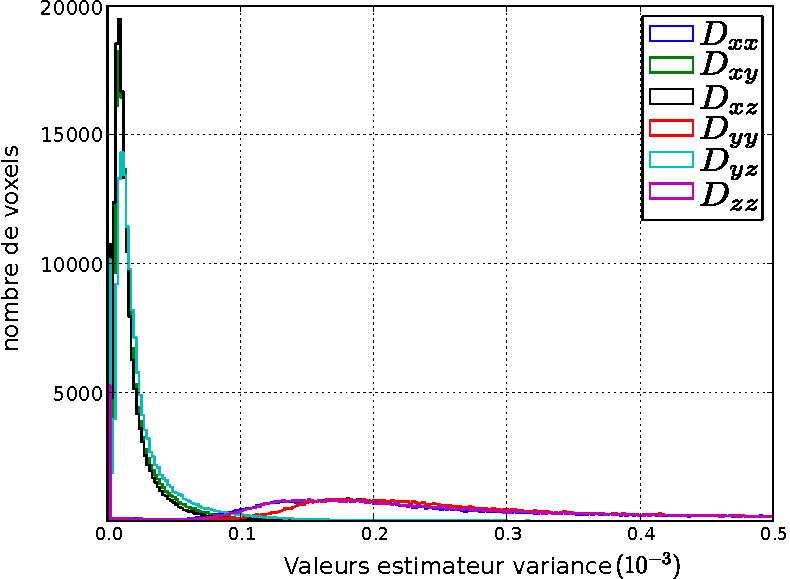
\includegraphics[scale=0.6]{Images/hist_var.pdf}
    \caption{\label{hist_var}Histogrammes des valeurs (en nombres de voxels) de l'estimateur de la variance $\sigma^2$ (en $10^{-3}$)
    pour chaque élément du tenseur.}
\end{figure}

Le modèle sous l'hypothèse d'hétéroscédasticité devient un cas d'observations multivariées 
où les tenseurs représentent les vecteurs d'observations.
La matrice des observations s'écrit alors simplement de la manière suivante :

\begin{equation}
    \underbrace{\mathbf{Y}_{}}_{N\times 1} = \left[\begin{array}{c}
                                             y_1\\
                                             \vdots\\
                                             y_N
                                         \end{array}\right]
  \xrightarrow{\text{devient}}
  \underbrace{\mathbf{Y}_{}}_{(N\times 6)} = \left[\begin{array}{ccccccccccccc}
                                             D^1_{xx} & D^1_{xy} & D^1_{xz} & D^1_{yy} & D^1_{yz} & D^1_{zz}\\
                                              & & & \vdots & & \\
                                             D^N_{xx} & D^N_{xy} & D^N_{xz} & D^N_{yy} & D^N_{yz} & D^N_{zz}\\
                                         \end{array}\right]
\end{equation}

Cette méthode est équivalente à indépendamment estimer six régressions univariées, une pour chaque élément du tenseur, 
avec la même matrice de dessin que pour l'application sur les image de \fa ($X\left[i,j\right] = x_{i,j} \text{, pour } i = 1\dots N \text{ et } j = 1\dots K$). 
Chacune de ses six régressions permet d'estimer les $K$ régresseurs associés à chaque composant du tenseur.
Cela conduit à l'estimation de six résidus au sens des moindres carrés $RSS_{t=1..6}$.
La question qui se pose à cette étape est : Comment fusionner les informations des six résidus $RSS_{t=1..6}$ ?
En effet, si nous appliquons le test de Fisher aux six résidus $RSS_{t=1..6}$, nous obtenons six scores différents.
Comment prendre en compte et quantifier ces six scores correctement ? 
La solution triviale de sélectionner un score (le plus grand ou le plus petit par exemple)
parmi les six valeurs revient à perdre l'apport d'information fourni par la prise e compte de tous les éléments du tenseur.
La méthode de combinaison des probabilités proposée par \cite{Whitlock2005} permet de s'affranchir de ce problème
en présentant un nouveau test fusionnant les \textit{p-valeurs} des six tests de Fisher précédent.\\
\begin{equation}
    z = \frac{\sum_{t=1}^{6} \Phi^{-1}(1-p_t)}{\sqrt{6}} 
    \label{fusion}
\end{equation}
avec $\Phi$ la fonction de répartition et $p_t$ la $t^\text{ième}$ \textit{p-valeur}.
L'équation \eqref{fusion} permet de calculer à nouveau un score qui suit une loi normal
$z\ \overset{iid}{\sim}\ \mathcal{N}(0, 1)$.
Ce test étant paramétrique, il est facile de calculer une nouvelle et unique \textit{p-valeur} représentant les six autres.
Dans la suite du manuscrit, cette méthode se nommera \mlg Multivarié pour les Tenseurs de Diffusion (\textit{MLG-M-TD}).


\subsection{Prise en compte des informations multi-échelles}
Dans les deux méthodes présentées dans les paragraphes précédents, seule l'information contenue dans un voxel est utilisée.
L'idée d'exploiter l'information présente dans les voxels voisins est pertinente et souvent utilisée en traitement d'images médicales \cite{Grigis2012}.
De même que l'idée de prendre en compte l'information du voxel à différentes résolutions : fine, normale et grossière.
Cette dernière façon de faire est utilisée de manière récurrente dans des méthodes de recalage \cite{Yap2009} ou d'extraction de caractéristiques.

Pour ce modèle, la méthode consiste à faire $G=3$ régressions univariées avec une hypothèse d'homoscedasticité sur le vecteur du tenseur. 
Ces régressions prennent comme observations les élements du tenseur avec trois niveaux de filtrages différents : la première utilise les observations brutes sans filtrage, la deuxième utilise un filtre d'une largeur normale (cela correspond au filtrage classique effectué sur les observations avant les deux méthodes précédentes) et la troisième régression utilise un filtrage plus large.
Toutes ces observations sont ensuite concaténées dans une seule matrice $\mathbf{Y}$ (voir équation \eqref{glm_echelle}).

\begin{equation}
    \underbrace{\mathbf{Y}_{}}_{N\times 1} = \left[\begin{array}{c}
                                             y_1\\
                                             \vdots\\
                                             y_N
                                         \end{array}\right]
  \xrightarrow{\text{devient}}
  \underbrace{\mathbf{Y}_{}}_{(N\times 6)\times G} = \left[\begin{array}{ccc}
                                             D^1_{xx} & D^{1,g}_{xx} & D^{1,G}_{xx}\\
                                             D^1_{xy} & D^{1,g}_{xy} & D^{1,G}_{xy}\\
                                             D^1_{xz} & D^{1,g}_{xz} & D^{1,G}_{xz}\\
                                             D^1_{yy} & D^{1,g}_{yy} & D^{1,G}_{yy}\\
                                             D^1_{yz} & D^{1,g}_{yz} & D^{1,G}_{yz}\\
                                             D^1_{zz} & D^{1,g}_{zz} & D^{1,G}_{zz}\\
                                             \vdots & \vdots & \vdots\\
                                             D^N_{xx} & D^{N,g}_{xx} & D^{N,G}_{xx}\\
                                             D^N_{xy} & D^{N,g}_{xy} & D^{N,G}_{xy}\\
                                             D^N_{xz} & D^{N,g}_{xz} & D^{N,G}_{xz}\\
                                             D^N_{yy} & D^{N,g}_{yy} & D^{N,G}_{yy}\\
                                             D^N_{yz} & D^{N,g}_{yz} & D^{N,G}_{yz}\\
                                             D^N_{zz} & D^{N,g}_{zz} & D^{N,G}_{zz}\\
                                         \end{array}\right]
  \label{glm_echelle}
\end{equation}

Par la suite, cette méthode est identique à celle avec l'hypothèse d'hétéroscédasticité. 
De la même manière, les $G$ \textit{p-valeurs} sont combinées par la méthode \cite{Whitlock2005}.
Elle sera nommée \mlg avec Voisinage pour les Tenseurs de Diffusion (\textit{MLG-V-TD}) dans la suite du document.


%    %%%%%%%%%%%%%%%%%%%%%%%%%%%%%%%%%%%%%%%%%%%%
% Chapitre 5
%%%%%%%%%%%%%%%%%%%%%%%%%%%%%%%%%%%%%%%%%%%%

\chapter{Variétés non linéaires}
\label{Chapter5}

% \minitoc

%----------------------------------------------------------------------------------------

\section{Problématique des métriques euclidiennes}
% \lipsum[22-26]
\section{Géométrie riemanienne}
% \lipsum[22-26]
\subsection{Principe}
\subsection{État de l'art des régressions sur cette variété}
\subsection{Méthode du "Multivariate General Linear Models"}
\subsubsection{Description de la méthode}
\subsubsection{Test statistique}

\section{Géométrie log-euclidienne}
\subsection{Principe}
\subsection{Application dans le cadre GLM-DT}


% \section{Conclusion partielle}

%    %%%%%%%%%%%%%%%%%%%%%%%%%%%%%%%%%%%%%%%%%%%%
% Chapitre 6
%%%%%%%%%%%%%%%%%%%%%%%%%%%%%%%%%%%%%%%%%%%%

\chapter{Caractérisation des changements}
\label{Chapter6}

Le \chapref{Chapter4} présente des méthodes de détection de changements entre deux populations de tenseurs.
Ces méthodes de comparaison de groupes permettent de détecter les régions pour lesquelles la forme des tenseurs de diffusion diffère 
significativement d'une population à l'autre, sans toutefois donner d'information sur la nature des changements observés.
Ainsi, une méthode complémentaire est proposée, permettant de caractériser a posteriori les changements détectés en termes de
modification de la Fraction d'Anisotropie (FA), Diffusion Moyenne (DM), Diffusion Radiale (DR) ou Diffusion
Axiale (DA), afin de rendre l'interprétation des résultats plus aisée pour le Neurologue.\\

% \minitoc

%----------------------------------------------------------------------------------------

\section{Post-traitement général}
Les cartes de \textit{p-valeurs} obtenues en sortie des méthodes de détection des changements sont dites \og brutes \fg,
c'est-à-dire sans avoir subies de transformations quelconques pour améliorer les détections.
Nous les appellerons par la suite \og cartes primaires \fg.
Il est possible d'appliquer, de manière systématique, des corrections statistiques et morphologiques à ces cartes.
Le post-traitement général présenté dans cette section est effectué en deux étapes : 
une correction statistique des cartes de \textit{p-valeurs} suivie d'une correction sur la topologie des détections.
Après ces corrections, la carte de résultats est appelée \og carte corrigée \fg.

\subsection{Correction statistique des cartes de p-valeurs}
Positionnons-nous dans le cas de la compraison de groupes en imagerie médicale.
Nous avons $N$ images-sujets comportant $V$ voxels chacune.
Le \mlg va réduire pour chaque voxel les $N$ informations en $K$ régresseurs et 
le test statistique va mesurer l'effet d'un de ces régresseurs pour chaque voxel.
En sortie, nous obtenons une carte de $V$ \textit{p-valeurs} (carte primaire de détection).
Durant ce processus, le test d'hypothèse \eqref{test_stat} est effectué $V$ fois.
Ces $V$ tests sont indépendants et pour chacun le niveau de signification est nommé $\alpha_{test}$. 
Il correspond à la probabilité de rejeter l'hypothèse nulle $\mathcal{H}_0$ alors qu'elle est vraie, 
ou encore à la probabilité de détecter un Faux Positif.
Sur ces $V$ tests, nous connaissons le nombre $A$ de décisions acceptant l'hypothèse $\mathcal{H}_0$ et le nombre $R$ la rejetant ($V=A+R$).
Trois cas sont possibles : \\
\begin{itemize}
    \item Sans aucune correction, un pourcentage $\alpha_{test}$ des $V$ voxels sont des Faux Positifs.\\
    
    \item Le premier type de correction sert à contrôler le nombre de Faux Positifs parmi le $V$ voxels.
    C'est la méthode de Bonferroni \cite{Abdi2007} (ou encore en anglais \textit{Family Wise Error Rate} FWER).
    Les $V$ tests sont indépendants donc la probabilité d'accepter l'hypothèse nulle $\mathcal{H}_0$ pour cette famille de test est : $(1-\alpha_{test})^V$.
    Il en découle directement la probabilité de rejeter $\mathcal{H}_0$ pour la famille de test : $\alpha_{famille} = 1 - (1-\alpha_{test})^V$.
    Par exemple, si $V=100$ et $\alpha_{test} =0.05$ alors $\alpha_{famille}=0,00592$.
    Pour une image classique du tenseur de diffusion avec une taille de $128\time128\time41$, nous avons $V=671744$ voxels.
    Alors la probabilité $\alpha_{famille}$ devient très petite, rendant la correction trop stricte.\\
    
    \item La deuxième méthode de correction va contrôler le nombre de Faux Positifs $FPos$ parmi les $R$ détections \cite{Benjamini1995, Benjamini2001}
    (en anglais \textit{False Discovery Rate} FDR).
    Il définit un taux de Faux Positif $taux_{FPos}$ et exprime le FDR comme l'espérance de ce taux devant être inférieur au niveau de signification $\alpha_{test}$ :
    \begin{align}
        taux_{FPos} &= \left\{ \begin{array}{lr} \frac{FPos}{R} & : R > 0\\ 0 & : sinon \end{array} \right.\\
        FDR &= E\left[taux_{FPos} \right] < \alpha_{test}
    \end{align}
    La procédure consiste à classer les $R$ \textit{p-valeurs} : $p_1 \leq p_2 \leq \dots p_R$ par ordre croissant.
    Et à rejeter les $k$ \textit{p-valeurs} (parmi les $R$) qui vérifient :
    \begin{equation}
        p_i \leq \frac{i}{V}\alpha_{test} 
    \end{equation}
    Avec cette correction, seuls $\alpha_{test}$ voxels sur les $R$ sont des fausses alarmes (Faux Positifs).
    Pour notre chaine de traitements, nous avons choisi cette correction.
\end{itemize}


\subsection{Composantes connexes}
La correction statistique permet de contrôler le taux de Faux Positifs sur l'image entière
mais ne fait aucune intervention par rapport à la morphologie des zones détectées.
Physiquement, il est facile de comprendre que les détections de voxels isolés ou encore des agrégats de voxels de toutes petites tailles, ne sont pas représentatifs d'une lésion 
car elles sont, de manière générale, plus étendues sur la substance blanche.
Par exemple, pour une image de résolution $1.8\time1.8\time3.5 mm^3$, une détection isolée (1 seule voxel) corresponderait à une lésion d'environ $12 mm^3$.
Ces détections sont souvent attribuées à de Faux Positifs.
Par la suite, il est préférable de ne conserver que les agrégats dont la taille est supérieure à celle fixée par l'utilisateur (voir \figref{etape_carac_1}).
Pour cela, nous utilisons la méthode des composantes connexes.
Ce sont des opérateurs de morphologie mathématique qui servent, généralement, d'outils de filtrage et de segmentation.

\begin{figure}[ht]
  \centering
  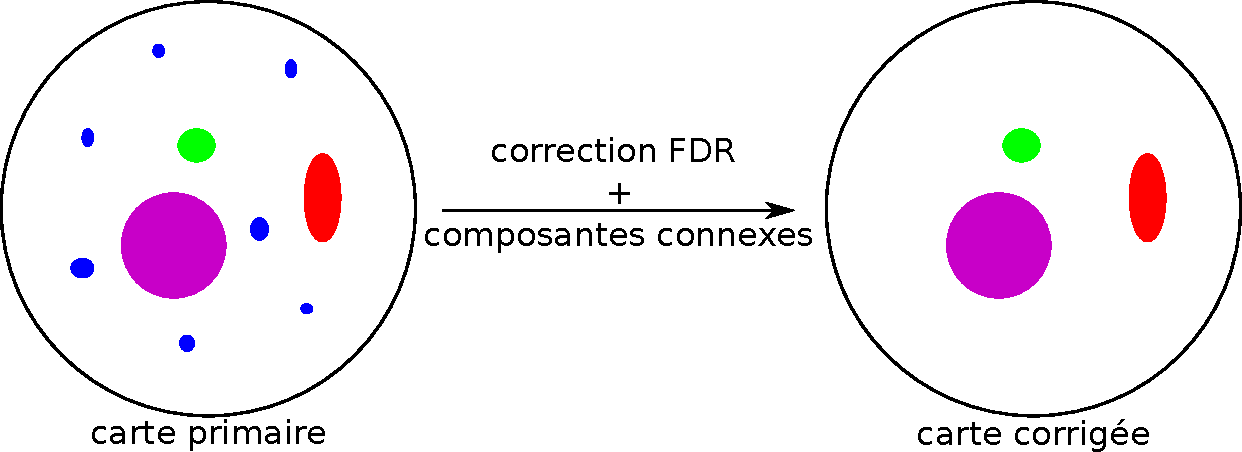
\includegraphics[scale=0.5]{Images/etape_carac_1.pdf}
  \caption{\label{etape_carac_1}Illustration du post-traitement général.}
\end{figure}


\section{Caractérisation des zones détectées}
Les méthode de comparaison de groupes basées sur les tenseurs sont des extension du \mlg.
Avec le test de Fisher introduit au \chapref{Chapter4}, une carte de \textit{p-valeurs} est obtenue.
Elle est ensuite corrigée par la méthode du False Discovery Rate (FDR), puis seuillée à un seuil de 5\%.
Cette approche permet d'identifier les régions atteintes par la pathologie, sans apporter d'information sur la nature et le sens des changements détectés.
Cette section présente une méthode de post-traitement pour pallier à la problématique des méthodes de détection.
Elle consiste à caractériser les détections obtenues avec les méthodes du \chapref{Chapter4}.


\subsection{Description de la méthode de caractérisation}
Les méthodes de comparaison de groupes permettent de prendre en compte toute l'information contenue dans les tenseurs sous différentes hypothèses
(homoscédasticité et hétéroscédasticité).
Pour chaque méthode, des régresseurs associé à chaque élément du tenseur, sont estimés au sens des moindres carrés.
Ensuite, un test statistique de Fisher est utilisé pour tester la significativité des effets de ces regresseurs dans les modèles.

La première étape (voir \figref{etape_carac_1}) de la caractérisation des changements consiste à corriger les cartes de détection par la méthode du FDR,
puis à étiqueter les composantes connexes de la carte des détections seuillée 
et à ne conserver que celles dont la taille est supérieure à un seuil fixé par l'utilisateur. 
Cette étape correspond aux opérations du post-traitement général.

\begin{figure}[ht]
    \centering
    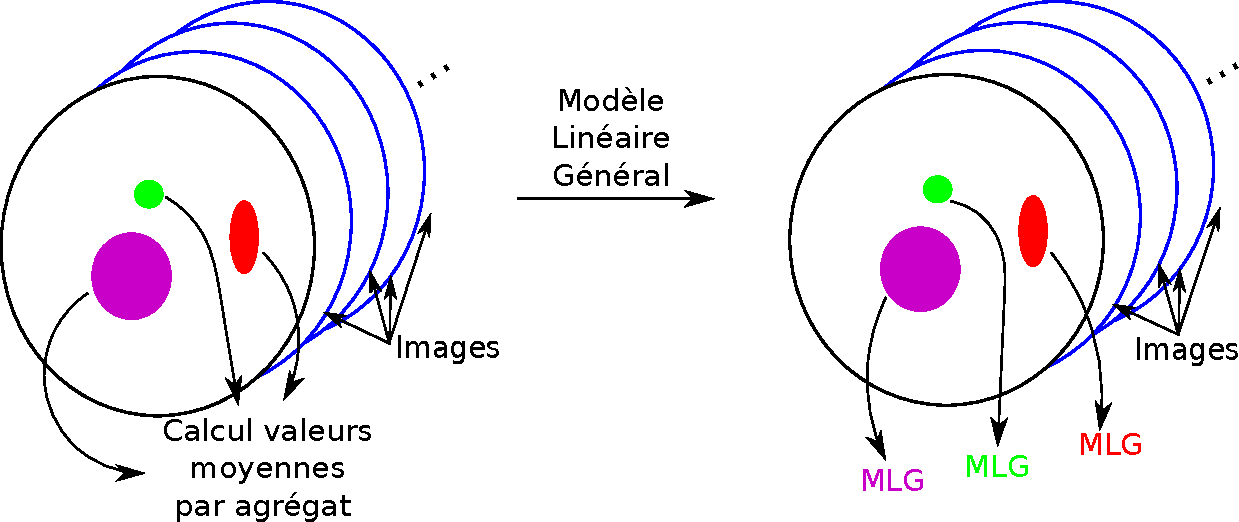
\includegraphics[scale=0.6]{Images/etape_carac_2.pdf}
    \caption{\label{etape_carac_2}Illustration de la deuxième étape de la caractérisation.}
\end{figure}
La deuxième étape (voir \figref{etape_carac_2}) consiste, sur chaque région et pour chaque sujet, à calculer les valeurs
moyennes des différents indices scalaires (\fa (FA), \md (DM), \dr (DR) et \da (DA)) et à comparer indépendemment chacune de ces quantités grâce à
un \mlg, en utilisant les même covariables que précédemment.

\begin{figure}[ht]
    \centering
    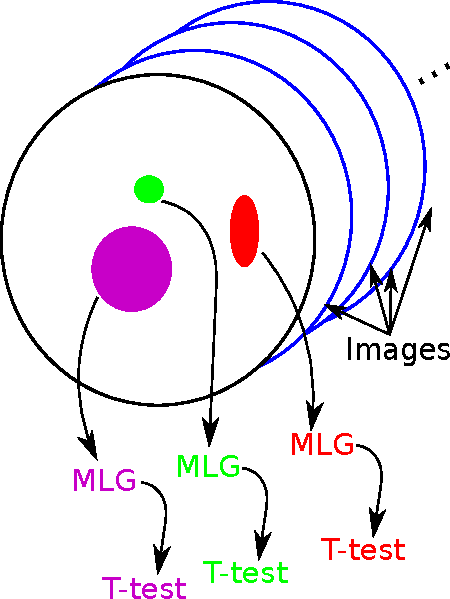
\includegraphics[scale=0.6]{Images/etape_carac_3.pdf}
    \caption{\label{etape_carac_3}Illustration de la troisième étape de la caractérisation.}
\end{figure}
Un test de Student, ou encore T-test, est réalisé pour chaque agrégat, afin d'identifier le sens du changement détecté (voir \figref{etape_carac_3}).
L'hypothèse nulle $\mathcal{H}_0$ vérifie $c^t \hat{B} =0 \text{ avec } c \in \mathbb{R}^{k}$ 
le vecteur de constraste permettant de faire une combinaison linéaire des régresseurs $\hat{B}$.
\begin{equation}
    t = \frac{c^t\hat{B}}{\sqrt{c^t\hat{\Sigma}c}} \sim T_{d=N-K}
\end{equation}
Contrairement au test statistique utilisé \eqref{test_stat} pour les méthodes de détection,
il est alors possible de tester l'équalité entre deux régresseurs en mettant à $1$ et $-1$ les contrastes associés aux deux régresseurs à l'étude et tous les autres contrastes à $0$.
Ou encore, nous pouvons tester si un régresseur n'a pas d'effet sur le modèle en mettant le constraste associé à $1$ et les autres à $0$ pour, par exemple, étudier la corrélation supposée entre un score clinique et les observations.

Il faut noter une différence par rapport au cadre statistique précédent.
Dans le cas de ce test, pour la comparaison de groupes, il faut deux variables explicatives pour les deux groupe $\{x_1, x_2\}$ 
afin d'estimer un régresseur représentant le premier groupe et un deuxième pour l'autre groupe.


\subsection{Format de présentation des résultats}
La liste de ces régions est présentée au médecin en respectant l'ordre suivant dans les indices scalaire : DA:\da, DR:\dr, DM:\md, FA:\fa.
Seules les régions ayant conduit à au moins un test significatif au seuil de 5\% sont conservées. 
Cette liste précise le sens de modification du test à l'aide de deux symboles : ($+$) pour une augmentation et ($-$) pour une diminution, 
ainsi que le niveau de signification : ($n.s.$) pour un résultats non significatif.
Un exemple fictif, correspondant au schéma de la \figref{etape_carac_3}, est donné par le \tabref{ex_caracterisation}.
Les trois agrégats violet, vert et rouge correspondent respectivement aux numéros {\color{purple}1}, {\color{green}2} et {\color{red}3}.

\begin{table}[ht]
\centering
\begin{tabular}{|D{2cm}|D{1cm}|D{1cm}|D{1cm}|D{1cm}|}
      \hline
      \textbf{Agrégats} & \textbf{DA} & \textbf{DR} & \textbf{DM }& \textbf{FA} \tabularnewline
      \hline
      {\color{purple}1} & $-$ & $n.s.$ & $-$ & $-$\tabularnewline
      {\color{green}2} & $n.s.$ & $+$ & $+$ & $-$\tabularnewline
      {\color{red}3} & $-$ & $-$ & $-$ & $n.s.$\tabularnewline
      \hline
  \end{tabular}
  \caption{\label{ex_caracterisation}Exemple de liste présentant les résultats de la caractérisation.}
\end{table}

Dans la littérature \cite{Harsan2006}, deux types de modification ont été reliés à des phénomènes biologiques provoqués 
par des pathologies dégénératives du système nerveux central chez l'homme :\\
\begin{itemize}
    \item une diminution de la \da peut représenter une modification axonale comme une réduction du diamètre de l'axone.
    Cela engendrera aussi une diminution de la \md et de la Fraction d'Anisotropie.
    Dans ce cas de figure, les changements détectés en \dr ne sont pas représentatifs de la modification et nous admettons qu'ils peuvent être $-/+/n.s.$.
    La combinaison des symboles est : \{$-$, $(-/+/n.s.)$, $-$, $-$\}\\
    \item une augmentation de la \dr peut représenter une dégradation de la couche de myéline.
    Nous parlons alors de démyélinisation.
    Cela entraine une augmentation de la \md et une diminution de la Fraction d'Anisotropie.
    Dans ce cas là, les modifications détectées pour l'indice scalaire \da ne correspondent pas à des cas réels et les trois symboles $-/+/n.s.$ peuvent leur être attribués.
    La combinaison des symboles est : \{$(-/+/n.s.)$, $+$, $+$, $-$\}\\
\end{itemize}

Certaines combinaisons de symboles, par exemple \{$-$, $-$, $-$, $n.s.$\} ou encore \{$-$, $-$, $-$, $+$\}, 
représentent des modifications qui ne peuvent être associées avec des cas réels.
Deux explications permettent de comprendre ces résultats.
Tout d'abord, les changements détectés correspondent à une modification de l'orientation de la diffusion ce qui est impossible à détecter avec les valeurs scalaires.
Ensuite, il est possibile que plusieurs modifications différentes soient présentes dans l'agrégat et en faisant la moyenne des valeurs scalaires, 
les différents changements se compensent les uns aux autres.


\begin{figure}[ht]
    \centering
    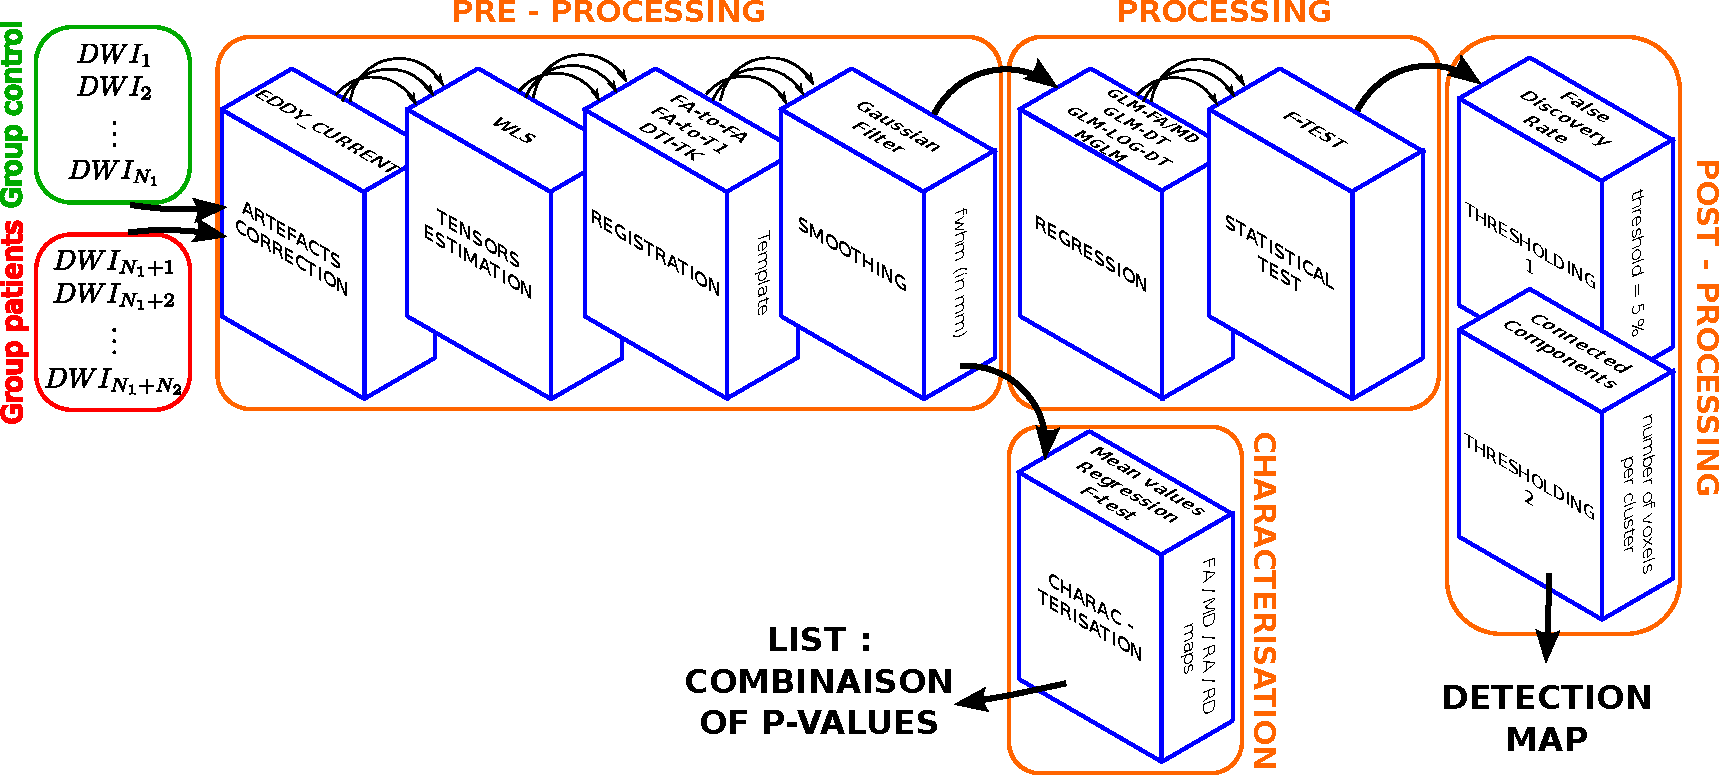
\includegraphics[width=1\textwidth]{Images/pipeline.pdf}
\end{figure}

%    
%      % partie 3
%    \part{Simulations et validations}
%    \label{Part3}
%    %%%%%%%%%%%%%%%%%%%%%%%%%%%%%%%%%%%%%%%%%%%%
% Chapitre 6
%%%%%%%%%%%%%%%%%%%%%%%%%%%%%%%%%%%%%%%%%%%%

\chapter{Cohortes de données utilisées}
\label{Chapter7} 

%    %%%%%%%%%%%%%%%%%%%%%%%%%%%%%%%%%%%%%%%%%%%%
% Chapitre 8
%%%%%%%%%%%%%%%%%%%%%%%%%%%%%%%%%%%%%%%%%%%%

\chapter{Évaluation de la méthode GLM-DT dans un cadre statistique Euclidien}
\label{Chapter8}

%    %%%%%%%%%%%%%%%%%%%%%%%%%%%%%%%%%%%%%%%%%%%%
% Chapitre 9
%%%%%%%%%%%%%%%%%%%%%%%%%%%%%%%%%%%%%%%%%%%%

\chapter{Influence du cadre statistique sur des méthodes basées tenseurs}
\label{Chapter9}

%    %%%%%%%%%%%%%%%%%%%%%%%%%%%%%%%%%%%%%%%%%%%%
% Chapitre 10
%%%%%%%%%%%%%%%%%%%%%%%%%%%%%%%%%%%%%%%%%%%%

\chapter{Influence des pré-traitements pour une comparaison de groupes}
\label{Chapter10}



% \minitoc

%----------------------------------------------------------------------------------------


\section{Recalage}
\section{Filtrage}
%    %%%%%%%%%%%%%%%%%%%%%%%%%%%%%%%%%%%%%%%%%%%%
% Chapitre 11
%%%%%%%%%%%%%%%%%%%%%%%%%%%%%%%%%%%%%%%%%%%%

\chapter{Contributions aux neurosciences}
\label{Chapter11}



% \minitoc

%----------------------------------------------------------------------------------------

\section{Sur la base de patients atteints de NMO}

\subsection{Résultats des méthodes linéaires}



% Fig. \ref{resNMO_1} shows the results obtained by the two scalar-based methods (\textit{GLM-FA} and \textit{GLM-MD}) and the Euclidean tensor-based method (\textit{GLM-DT})
% for the comparison between 34 NMO patients and 22 healthy subjects. 
% 
% The methods \textit{GLM-MD} and \textit{GLM-DT} present very similar results. 
% This observation is confirmed with the Dice coefficient always superior to $0.7$ for a wide range of thresholds (Fig. \ref{dice}).
% The main difference between the two methods concerns the putamen, which is a structure that has already been reported as involved in NMO~\cite{Zhao2012}
% and which is only detected by the  \textit{GLM-DT} and not by the \textit{GLM-MD}.
% The \textit{GLM-FA} method has a significantly different behavior as compared to  \textit{GLM-MD} and \textit{GLM-DT} (Fig. \ref{dice}).
% The most prominent difference  is that \textit{GLM-FA} does not detect alterations in the body of the corpus callosum and in the
% occipital lobe, which are structures that have also already been reported as involved in NMO~\cite{Yu2008,Rueda2012,Zhao2012}.
% 
% Finally, the major difference between the three methods concerns the statistical threshold requires to detect the 5\% of the most significant voxels within the white matter.
% The corresponding $p$-value thresholds are $p_{GLM-FA}=0.02$, $p_{GLM-MD}=0.04$ and $p_{GLM-DT}=0.002$.
% Consequently, \textit{GLM-DT} clearly outperforms the two other methods in terms of statistical power. Notice that for a $p$-value threshold of $0.002$,
% neither  \textit{GLM-FA}  nor  \textit{GLM-MD}  can detect any change. This gain in statistical power is explained by the fact that \textit{GLM-DT} relies on six times more data samples than the scalar-based methods.


\begin{figure*}[ht]
    \centering
    \includegraphics[width=0.9\textwidth]{Images/res_NMO_scalar_vs_tensor_annotations.pdf}
    \caption{\label{fig:nmo_1} Comparaison entre les méthodes basées sur les indices scalaires (\textit{GLM-FA} and \textit{GLM-MD}) 
    et la méthode basée sur les tenseurs avec une métrique Euclidienne (\textit{GLM-DT}).
    Les cartes statistiques sont seuillées de telle façon que seuls 5\% des voxels les plus significatifs dans le masque de la substance blanche sont retenus.
    La méthode des composantes connexes élimine les agrégats de taille inférieure à $N_c=10$ voxels.}
\end{figure*}

\subsection{Résultats des deux variétés géométriques}


\begin{figure*}[ht]
    \centering
    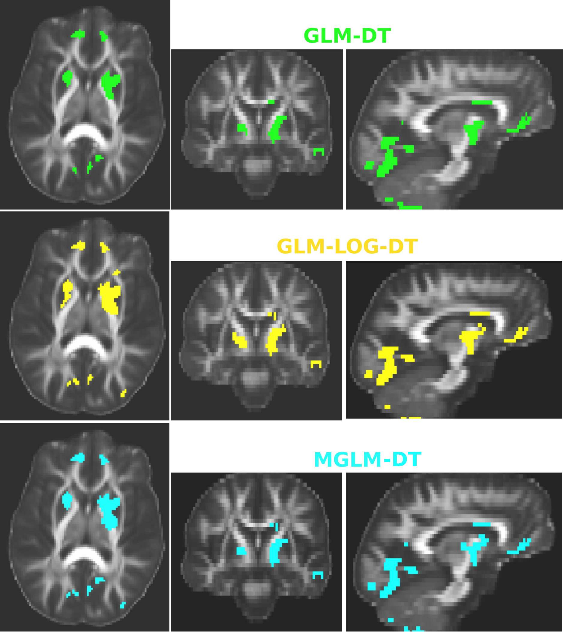
\includegraphics[width=0.8\textwidth]{Images/res_NMO_manifolds_annotations.pdf}
    \caption{\label{fig:nmo_2} Influence sur les méthodes basées tenseur de la métrique utilisée pour la comparaison de groupe entre les patients atteints de la NMO et les sujets contrôles.
    Les cartes statistiques sont seuillées de telle façon que seuls 5\% des voxels les plus significatifs dans le masque de la substance blanche sont retenus.
    La méthode des composantes connexes élimine les agrégats de taille inférieure à $N_c=10$ voxels.}
\end{figure*}


\subsection{Caractérisation}
La méthode de caractérisation est appliquée sur les cartes de détection obtenues avec la méthode \textit{GLM-DT}.
Au préalable, ces cartes dites \og primaires \fg sont corrigées par un FDR avec une seuil de $p_{FDR}=0.05$
et un technique de composantes connexes termine d'éliminer les détections résiduelles en ne conservant que les agrégats de taille supérieure à $N_c=10$.
Cette caractérisation appliquée à la carte primaire de la comparaison de sujets NMO \textit{vs} sujets sains, 
conduit à détecter 19 agrégats localisés sur 8 régions anatomiques différentes.

Le \tabref{tab:caracterisation} présente la liste de tous ces agrégats avec comme information : 
\begin{itemize}
    \item la région anatomique où se situe l'agrégat avec en information supplémentaire le côté,
    \item le (ou les) faisceau de la substance blanche touché,
    \item le signe du changement détecté :
    \begin{itemize}
        \item un \og $+$ \fg lorsqu'il s'agit d'un augmentation chez les sujets atteints par rapport aux sujets sains,
        \item un \og $-$ \fg dans le cas d'une diminution chez les sujets atteints par rapport aux sujets sains,
        \item une abbréviation \og n.s. \fg lorsque l'agrégat n'est pas significatif pour l'indice scalaire étudié.
    \end{itemize}
\end{itemize}



% Moreover the sign and the statistical significance ($p<0.05$) of the change for each scalar index (MD and FA) and each cluster are reported (see Table \ref{tab:characterisation2}).
% 
% The results show eight clusters classified as deleterious changes, four as favorable changes and seven as uncategorisable changes.
% 
% Five clusters in the occipital lobe are characterized by an augmentation of the mean diffusivity in the patient group as compared to the control group, 
% which may reflect a demyelination that is probably related to the visual disorders induced by the pathology.
% Similar signatures are observed for clusters located in the hippocampus and the corpus callosum.
% Two clusters, respectively in the parietal lobe and the frontal lobe 
% (cluster on the left inferior fronto-occipital tract and the genu of the corpus callosum) 
% present a radial diffusion augmentation and an axial diffusion diminution which can also be linked to a demyelination process.
% The four clusters that are categorized as favorable changes might be the consequences of compensation phenomena or therapeutic drugs effects.
% The remaining clusters belong to the uncategorisable group.
% 
% We are well aware that there are multiple others options to process this kind of classification.
% We choose this direct way to do because of the procedure user friendlyness, the computational efficiency 
% and the similar approach of the detection method (both based on the GLM with the same covariables).

\begin{table}[htbp]
\centering
\begin{tabular}{|D{3.5cm}|D{0.5cm}|D{4.5cm}|D{1.2cm}|D{1.2cm}|}
      \hline
      \multicolumn{2}{|c|}{\textbf{Localisation}} & \textbf{Faisceau impacté} & \textbf{MD} & \textbf{FA} \tabularnewline
      \hline
      \hline
      \multirow{5}{*}{Lobe occipital} & d. & optic radiation \\ faisceau long. inf. \\ corps calleux (splenium) & $+$ & $n.s.$ \tabularnewline
       \cline{2-5}
       & g. & optic radiation \\ corps calleux (splenium) & $+$ & $n.s.$ \tabularnewline
       \cline{2-5}
       & g. & optic radiation \\ inf. long. fasciculus \ corps calleux (splenium) & $+$ & $n.s.$ \tabularnewline
       \cline{2-5}
       & d. & inf. fronto-occipital fasciculus & $+$ & $n.s.$ \tabularnewline
       \cline{2-5}
       & d. & \cellcolor[gray]{0.9} & $n.s.$ & $n.s.$ \tabularnewline
      \hline
      Hippocampe & g. & \cellcolor[gray]{0.9} & $+$ & $n.s.$ \tabularnewline
      \hline
      Corps calleux & d. & corps calleux (body) & $+$ & $n.s.$ \tabularnewline
      \hline
      Lobe pariétal & d. & faisceau long. sup. & $+$ & $-$ \tabularnewline
      \hline
      \multirow{3}{*}{Lobe frontal} & g. & corps calleux (genu) \\ inf. fronto-occipital & $-$ & $-$ \tabularnewline
       \cline{2-5}
       & d. & inf. fronto-occipital & $n.s.$ & $n.s.$ \tabularnewline
       \cline{2-5}
       & g. & corps calleux (genu) & $-$ & $+$ \tabularnewline
      \hline
      \multirow{2}{*}{Capsule interne} & d. & inf. fronto-occipital\\ dentate-rubro-thalamo cortical & $n.s.$ & $n.s.$ \tabularnewline
       \cline{2-5}
       & d. & faisceau cortico-spinal & $-$ & $n.s.$ \tabularnewline
      \hline
      \multirow{2}{*}{Lobe temporal} & d. & faisceau arcqué & $n.s.$ & $n.s.$ \tabularnewline
       \cline{2-5}
       & d. & faisceau long. inf. & $-$ & $n.s.$ \tabularnewline
      \hline
      \multirow{4}{*}{Cervelet} & d. & \cellcolor[gray]{0.9} & $-$ & $n.s.$ \tabularnewline
       \cline{2-5}
       & g. & \cellcolor[gray]{0.9} & $n.s.$ & $n.s.$ \tabularnewline
       \cline{2-5}
       & g. & \cellcolor[gray]{0.9} & $n.s.$ & $n.s.$ \tabularnewline
       \cline{2-5}
       & d. & \cellcolor[gray]{0.9} & $n.s.$ & $n.s.$ \tabularnewline
      \hline
  \end{tabular}
  \caption{\label{tab:caracterisation} Résultats ($p_\text{corrigées}<0.05$) de la caractérisation pour la méthode \textit{GLM-DT} (seuil statistique $p_{FDR}=0.05$ et seuil $N_c=10$).
  (Légende: $+=$ augmentation significative, $-=$ diminution significative, $n.s.=$ non significatif, d. $=$ droite, l. $=$ gauche, inf. $=$ inférieur, sup. $=$ supérieur, long. $=$ longitudinale)}
\end{table}

\section{Sur la base de patients atteints de DLB}
\subsection{Comparaison de patients au stade prodomal avec des témoins}
\subsection{Étude sur les hallucinations dans le maladie à corps de Lewy}



    
%    \part{Conclusion}
%    \label{Conclu}
%    
    
    \pagestyle{introduction}
      % bibliographie
    \biblio{Bibliography}
    \label{Biblio}
    \bibliographystyle{mn2e}
    \bibliography{Bibliography/bibdatabase}
%     \addstarredchapter{\textsc{Bibliographie}}
    \markboth{\textsc{Bibliography}}{}
    
    \backmatter
    \listoffigures
%     \addstarredchapter{Liste des figures}
    \listoftables
%     \addstarredchapter{Liste des tableaux}
%     
%     \appendix


\end{document}
